\fancyhead[LH]{复旦大学软件工程}
\fancyhead[RH]{第四章\quad 用况建模}
\section{用况建模}

% \subsection{领域概念模型}


\subsection{确定执行者}
由于Volunet志愿服务系统过于庞大,在整个系统上去确定执行者将变得较为困难。故我们沿用需求分析中对其的系统拆解,分为信息管理系统、志愿服务系统、爱心捐助系统、公益课程系统、交流论坛系统、志愿交友系统六个部分,再在这六个子系统下确定各自相关的执行者。

\subsubsection{信息管理系统执行者}
信息管理系统的执行者包括:志愿团队、志愿者、系统管理员。其中,使用信息管理系统的人或组织有志愿团队、志愿者、系统管理员,这些人、组织都是信息管理系统的执行者。

信息管理系统的执行者及其词条描述如下:

\begin{table}[H]  
\caption{“志愿者”执行者词条描述}  
\begin{center}  
    \begin{tabular}{l p{11cm}} 
        \hline
        \quad 名称:  & 志愿者 \\
        \hline
        \quad 身份:  & 主执行者 \\
        \hline
        \quad 简述:  & 参与志愿活动的人 \\
        \hline
        \quad 功能:  & 主动执行者 \\
        \hline
        \quad 相关用况:  & 组队管理、注册管理、用户管理 \\
        \hline
    \end{tabular}
\end{center}
\end{table}

\begin{table}[H]  
\caption{“志愿团队”执行者词条描述}  
\begin{center}  
    \begin{tabular}{l p{11cm}} 
        \hline
        \quad 名称:  &   志愿团队 \\
        \hline
        \quad 身份:  & 主执行者 \\
        \hline
        \quad 简述:  & 发布和组织志愿活动的组织 \\
        \hline
        \quad 功能:  & 主动执行者 \\
        \hline
        \quad 相关用况:  & 团队管理、组队管理 \\
        \hline
    \end{tabular}
\end{center}
\end{table}


\begin{table}[H]  
\caption{“系统管理员”执行者词条描述}  
\begin{center}  
    \begin{tabular}{l p{11cm}} 
        \hline
        \quad 名称:  &  系统管理员 \\
        \hline
        \quad 身份:  & 副执行者 \\
        \hline
        \quad 简述:  & 负责信息审核和权限管理的人 \\
        \hline
        \quad 功能:  & 被动执行者 \\
        \hline
        \quad 相关用况:  & 信息审核、用户限权 \\
        \hline
    \end{tabular}
\end{center}
\end{table}


\subsubsection{志愿服务系统执行者}
志愿服务系统的执行者包括:志愿团队、志愿者、审核员。
定位打卡系统 交流论坛系统。其中,使用志愿服务系统的人或组织有志愿团队、志愿者、审核员,与爱心捐助交互的其他外部系统有获取当前定位信息的定位打卡系统,这些人、组织和外部系统都是志愿服务系统的执行者。

志愿服务为系统的执行者及其词条描述如下:

\begin{table}[H]  
\caption{“志愿团队”执行者词条描述}  
\begin{center}  
    \begin{tabular}{l p{11cm}} 
        \hline
        \quad 名称:  & 志愿团队 \\
        \hline
        \quad 身份:  & 主执行者 \\
        \hline
        \quad 简述:  & 申请志愿服务项目,对志愿者报名单进行筛选,获得活动开展情况的组织 \\
        \hline
        \quad 功能:  & 主动执行者 \\
        \hline
        \quad 相关用况:  & 项目发布、项目报名、项目管理 \\
        \hline
    \end{tabular}
\end{center}
\end{table}

\begin{table}[H]  
\caption{“志愿者”执行者词条描述}  
\begin{center}  
    \begin{tabular}{l p{11cm}} 
        \hline
        \quad 名称:  &   志愿者 \\
        \hline
        \quad 身份:  & 主执行者 \\
        \hline
        \quad 简述:  & 浏览发布的志愿服务项目,报名参与感兴趣的项目,在项目过程中完成签到签退以及反馈的人 \\
        \hline
        \quad 功能:  & 主动执行者 \\
        \hline
        \quad 相关用况:  & 项目报名、项目管理 \\
        \hline
    \end{tabular}
\end{center}
\end{table}

\begin{table}[H]  
\caption{“系统管理员”执行者词条描述}  
\begin{center}  
    \begin{tabular}{l p{11cm}} 
        \hline
        \quad 名称:  &  系统管理员 \\
        \hline
        \quad 身份:  & 副执行者 \\
        \hline
        \quad 简述:  & 对志愿团队发布的项目进行审核的人 \\
        \hline
        \quad 功能:  & 被动执行者 \\
        \hline
        \quad 相关用况:  & 审核材料 \\
        \hline
    \end{tabular}
\end{center}
\end{table}

\begin{table}[H]  
\caption{“定位打卡系统”执行者词条描述}  
\begin{center}  
    \begin{tabular}{l p{11cm}} 
        \hline
        \quad 名称:  &  定位打卡系统 \\
        \hline
        \quad 身份:  & 副执行者 \\
        \hline
        \quad 简述:  & 获取手机当前定位信息和时间戳作为打卡标记的系统 \\
        \hline
        \quad 功能:  & 被动执行者 \\
        \hline
        \quad 相关用况:  & 项目管理 \\
        \hline
    \end{tabular}
\end{center}
\end{table}



\subsubsection{爱心捐助系统执行者}


爱心捐助系统的执行者包括:志愿团队、捐款者、购买者、公益商户、系统管理员、快递配送系统、收费管理系统。其中,使用爱心捐助系统的人或组织有捐款者、购买者、志愿团队、公益商户、系统管理员,与爱心捐助交互的其他外部系统有负责订单快递配送的快递配送系统、对捐款和货款进行管理的收费管理系统,这些人、组织和外部系统都是爱心捐助系统的执行者。

爱心捐助系统的执行者及其词条描述如下:

\begin{table}[H]  
\caption{“捐款者”执行者词条描述}  
\begin{center}  
    \begin{tabular}{l p{11cm}} 
        \hline
        \quad 名称:  &   捐款者 \\
        \hline
        \quad 身份:  & 主执行者 \\
        \hline
        \quad 简述:  & 为志愿项目捐款的人 \\
        \hline
        \quad 功能:  & 主动执行者 \\
        \hline
        \quad 相关用况:  & 捐款管理、爱心反馈管理 \\
        \hline
    \end{tabular}
\end{center}
\end{table}

\begin{table}[H]  
\caption{“志愿团队”执行者词条描述}  
\begin{center}  
    \begin{tabular}{l p{11cm}} 
        \hline
        \quad 名称:  &   志愿团队 \\
        \hline
        \quad 身份:  & 副执行者 \\
        \hline
        \quad 简述:  & 发布资助项目,接收捐助的组织 \\
        \hline
        \quad 功能:  & 被动执行者 \\
        \hline
        \quad 相关用况:  & 捐款管理 \\
        \hline
    \end{tabular}
\end{center}
\end{table}

\begin{table}[H]  
\caption{“购买者”执行者词条描述}  
\begin{center}  
    \begin{tabular}{l p{11cm}} 
        \hline
        \quad 名称:  &   购买者 \\
        \hline
        \quad 身份:  & 主执行者 \\
        \hline
        \quad 简述:  & 购买公益商品的人 \\
        \hline
        \quad 功能:  & 主动执行者 \\
        \hline
        \quad 相关用况:  & 订单管理、爱心反馈管理 \\
        \hline
    \end{tabular}
\end{center}
\end{table}

\begin{table}[H]  
\caption{“公益商户”执行者词条描述}  
\begin{center}  
    \begin{tabular}{l p{11cm}} 
        \hline
        \quad 名称:  &  公益商户 \\
        \hline
        \quad 身份:  & 副执行者 \\
        \hline
        \quad 简述:  & 提供并售卖公益商品的人 \\
        \hline
        \quad 功能:  & 被动执行者 \\
        \hline
        \quad 相关用况:  & 订单管理 \\
        \hline
    \end{tabular}
\end{center}
\end{table}

\begin{table}[H]  
\caption{“系统管理员”执行者词条描述}  
\begin{center}  
    \begin{tabular}{l p{11cm}} 
        \hline
        \quad 名称:  &  系统管理员 \\
        \hline
        \quad 身份:  & 副执行者 \\
        \hline
        \quad 简述:  & 负责信息审核的人 \\
        \hline
        \quad 功能:  & 被动执行者 \\
        \hline
        \quad 相关用况:  & 信息审核 \\
        \hline
    \end{tabular}
\end{center}
\end{table}

\begin{table}[H]  
\caption{“快递配送系统”执行者词条描述}  
\begin{center}  
    \begin{tabular}{l p{11cm}} 
        \hline
        \quad 名称:  &  快递配送系统 \\
        \hline
        \quad 身份:  & 副执行者 \\
        \hline
        \quad 简述:  & 负责订单快递配送的系统 \\
        \hline
        \quad 功能:  & 被动执行者 \\
        \hline
        \quad 相关用况:  & 快递发货 \\
        \hline
    \end{tabular}
\end{center}
\end{table}

\begin{table}[H]  
\caption{“收费管理系统”执行者词条描述}  
\begin{center}  
    \begin{tabular}{l p{11cm}} 
        \hline
        \quad 名称:  &  收费管理系统 \\
        \hline
        \quad 身份:  & 副执行者 \\
        \hline
        \quad 简述:  & 对捐款和货款进行管理的系统 \\
        \hline
        \quad 功能:  & 被动执行者 \\
        \hline
        \quad 相关用况:  & 支付、退款、项目募捐 \\
        \hline
    \end{tabular}
\end{center}
\end{table}

\subsubsection{公益课程系统执行者}

公益课程系统的执行者包括:志愿者、授课人、系统管理员、反馈管理系统、修读管理系统、授课管理系统。

公益课程系统的执行者及其词条描述如下:


\begin{table}[H]  
\caption{“志愿者”执行者词条描述}  
\begin{center}  
    \begin{tabular}{l p{11cm}} 
        \hline
        \quad 名称:  &   志愿者 \\
        \hline
        \quad 身份:  & 主执行者 \\
        \hline
        \quad 简述:  & 选择课程、学习课程、进行反馈的人 \\
        \hline
        \quad 功能:  & 主动执行者 \\
        \hline
        \quad 相关用况:  & 修读管理、反馈管理、证书管理 \\
        \hline
    \end{tabular}
\end{center}
\end{table}

\begin{table}[H]  
\caption{“授课人”执行者词条描述}  
\begin{center}  
    \begin{tabular}{l p{11cm}} 
        \hline
        \quad 名称:  &   授课人 \\
        \hline
        \quad 身份:  & 主执行者 \\
        \hline
        \quad 简述:  & 发布课程,查看学生的反馈 \\
        \hline
        \quad 功能:  & 主动执行者 \\
        \hline
        \quad 相关用况:  & 证书管理、反馈管理、授课管理 \\
        \hline
    \end{tabular}
\end{center}
\end{table}

\begin{table}[H]  
\caption{“系统管理员”执行者词条描述}  
\begin{center}  
    \begin{tabular}{l p{11cm}} 
        \hline
        \quad 名称:  &  系统管理员 \\
        \hline
        \quad 身份:  & 副执行者 \\
        \hline
        \quad 简述:  & 负责授课资质和反馈审核的人 \\
        \hline
        \quad 功能:  & 被动执行者 \\
        \hline
        \quad 相关用况:  & 反馈管理、授课管理 \\
        \hline
    \end{tabular}
\end{center}
\end{table}

\begin{table}[H]  
\caption{“反馈管理系统”执行者词条描述}  
\begin{center}  
    \begin{tabular}{l p{11cm}} 
        \hline
        \quad 名称:  &  反馈管理系统 \\
        \hline
        \quad 身份:  & 副执行者 \\
        \hline
        \quad 简述:  & 负责反馈收集、处理、查询的系统 \\
        \hline
        \quad 功能:  & 被动执行者 \\
        \hline
        \quad 相关用况:  & 发布反馈、查看反馈、修改反馈、删除反馈 \\
        \hline
    \end{tabular}
\end{center}
\end{table}

\begin{table}[H]  
\caption{“修读管理系统”执行者词条描述}  
\begin{center}  
    \begin{tabular}{l p{11cm}} 
        \hline
        \quad 名称:  &  修读管理系统 \\
        \hline
        \quad 身份:  & 副执行者 \\
        \hline
        \quad 简述:  & 对志愿者选择课程进行管理和对志愿者学习课程进行记录的系统 \\
        \hline
        \quad 功能:  & 被动执行者 \\
        \hline
        \quad 相关用况:  & 申请课程、学习课程、考核课程、进行练习 \\
        \hline
    \end{tabular}
\end{center}
\end{table}


\begin{table}[H]  
\caption{“授课管理系统”执行者词条描述}  
\begin{center}  
    \begin{tabular}{l p{11cm}} 
        \hline
        \quad 名称:  &  授课管理系统 \\
        \hline
        \quad 身份:  & 副执行者 \\
        \hline
        \quad 简述:  & 对授课人教授课程进行管理的系统 \\
        \hline
        \quad 功能:  & 被动执行者 \\
        \hline
        \quad 相关用况:  & 授课申请、发布课程、修改课程、查询学生修读情况 \\
        \hline
    \end{tabular}
\end{center}
\end{table}

\subsubsection{交流论坛系统执行者}

交流论坛系统的执行者包括:用户、系统管理员。

交流论坛系统的执行者及其词条描述如下:

\begin{table}[H]  
\caption{“用户”执行者词条描述}  
\begin{center}  
    \begin{tabular}{l p{11cm}} 
        \hline
        \quad 名称:  &  用户 \\
        \hline
        \quad 身份:  & 主执行者 \\
        \hline
        \quad 简述:  & 进行志愿信息交流的人 \\
        \hline
        \quad 功能:  & 主动执行者 \\
        \hline
        \quad 相关用况:  & 资讯管理、手记管理、论坛管理 \\
        \hline
    \end{tabular}
\end{center}
\end{table}

\begin{table}[H]  
\caption{“系统管理员”执行者词条描述}  
\begin{center}  
    \begin{tabular}{l p{11cm}} 
        \hline
        \quad 名称:  &  系统管理员 \\
        \hline
        \quad 身份:  & 副执行者 \\
        \hline
        \quad 简述:  & 负责审核审计的人 \\
        \hline
        \quad 功能:  & 被动执行者 \\
        \hline
        \quad 相关用况:  & 发布审核、审计报告生成\\
        \hline
    \end{tabular}
\end{center}
\end{table}


\subsubsection{志愿交友系统执行者}

志愿交友系统的执行者包括:志愿者、交友申请、消息发送、消息接收、交友管理系统、消息管理系统。

志愿交友系统的执行者及其词条描述如下:


\begin{table}[H]  
\caption{“志愿者”执行者词条描述}  
\begin{center}  
    \begin{tabular}{l p{11cm}} 
        \hline
        \quad 名称:  &   志愿者 \\
        \hline
        \quad 身份:  & 主执行者 \\
        \hline
        \quad 简述:  & 查看用户、发送和处理好友申请的人 \\
        \hline
        \quad 功能:  & 主动执行者 \\
        \hline
        \quad 相关用况:  & 交友管理、消息管理 \\
        \hline
    \end{tabular}
\end{center}
\end{table}

\begin{table}[H]  
\caption{“交友申请”执行者词条描述}  
\begin{center}  
    \begin{tabular}{l p{11cm}} 
        \hline
        \quad 名称:  &   交友申请 \\
        \hline
        \quad 身份:  & 主执行者 \\
        \hline
        \quad 简述:  & 给其他非好友用户发送添加好友申请的人 \\
        \hline
        \quad 功能:  & 主动执行者 \\
        \hline
        \quad 相关用况:  & 交友管理、添加好友 \\
        \hline
    \end{tabular}
\end{center}
\end{table}

\begin{table}[H]  
\caption{“消息发送”执行者词条描述}  
\begin{center}  
    \begin{tabular}{l p{11cm}} 
        \hline
        \quad 名称:  &   消息发送 \\
        \hline
        \quad 身份:  & 主执行者 \\
        \hline
        \quad 简述:  & 给好友发送聊天消息的人 \\
        \hline
        \quad 功能:  & 主动执行者 \\
        \hline
        \quad 相关用况:  & 消息管理、发送消息 \\
        \hline
    \end{tabular}
\end{center}
\end{table}

\begin{table}[H]  
\caption{“消息接收”执行者词条描述}  
\begin{center}  
    \begin{tabular}{l p{11cm}} 
        \hline
        \quad 名称:  &   消息接收 \\
        \hline
        \quad 身份:  & 主执行者 \\
        \hline
        \quad 简述:  & 接收好友消息的人 \\
        \hline
        \quad 功能:  & 被动执行者 \\
        \hline
        \quad 相关用况:  & 消息管理、浏览消息 \\
        \hline
    \end{tabular}
\end{center}
\end{table}

\begin{table}[H]  
\caption{“交友管理系统”执行者词条描述}  
\begin{center}  
    \begin{tabular}{l p{11cm}} 
        \hline
        \quad 名称:  &  交友管理系统 \\
        \hline
        \quad 身份:  & 副执行者 \\
        \hline
        \quad 简述:  & 负责查询用户、处理好友申请的系统 \\
        \hline
        \quad 功能:  & 被动执行者 \\
        \hline
        \quad 相关用况:  & 交友管理、浏览好友、添加好友、删除好友 \\
        \hline
    \end{tabular}
\end{center}
\end{table}

\begin{table}[H]  
\caption{“消息管理系统”执行者词条描述}  
\begin{center}  
    \begin{tabular}{l p{11cm}} 
        \hline
        \quad 名称:  &  消息管理系统 \\
        \hline
        \quad 身份:  & 副执行者 \\
        \hline
        \quad 简述:  & 对好友之间收发消息进行管理的系统 \\
        \hline
        \quad 功能:  & 被动执行者 \\
        \hline
        \quad 相关用况:  & 消息管理,发送消息,接收消息 \\
        \hline
    \end{tabular}
\end{center}
\end{table}

\subsection{确定用况}

\subsubsection{信息管理系统用况}

信息管理系统针对志愿服务主体(志愿者和志愿团队)的账号和操作进行全流程的管理,包括用户管理、注册管理、组队管理、团队管理和信息审核。

信息管理系统的用况及其词条简述如下:
\begin{table}[H]  
\caption{“用户管理”用况词条简述}  
\begin{center}  
    \begin{tabular}{l p{11cm}} 
        \hline
        \quad 名称:  & 用户管理 \\
        \hline
        \quad 简要描述:  & 对志愿者用户的信息进行管理的过程 \\
        \hline
        \quad 分解用况:  & 用户登陆、用户查询、用户限权 \\
        \hline
        \quad 相关执行者:  & 志愿者、系统管理员 \\
        \hline
    \end{tabular}
    \label{tab1}
\end{center}
\end{table}

\begin{table}[H]  
\caption{“注册管理”用况词条简述}  
\begin{center}  
    \begin{tabular}{l p{11cm}} 
        \hline
        \quad 名称:  & 注册管理 \\
        \hline
        \quad 简要描述:  & 对志愿者用户的账号进行注册管理的过程 \\
        \hline
        \quad 分解用况:  & 填写注册信息、注册信息入库、注册反馈、修改注册信息 \\
        \hline
        \quad 相关执行者:  & 志愿者、系统管理员 \\
        \hline
    \end{tabular}
    \label{tab1}
\end{center}
\end{table}

\begin{table}[H]  
\caption{“组队管理”用况词条简述}  
\begin{center}  
    \begin{tabular}{l p{11cm}} 
        \hline
        \quad 名称:  & 组队管理 \\
        \hline
        \quad 简要描述:  & 对志愿者加入志愿团队进行管理的过程 \\
        \hline
        \quad 分解用况:  & 入队反馈、入队申请、团队展示、入队查询条件 \\
        \hline
        \quad 相关执行者:  & 志愿者、志愿团队、系统管理员 \\
        \hline
    \end{tabular}
    \label{tab1}
\end{center}
\end{table}

\begin{table}[H]  
\caption{“团队管理”用况词条简述}  
\begin{center}  
    \begin{tabular}{l p{11cm}} 
        \hline
        \quad 名称:  & 团队管理 \\
        \hline
        \quad 简要描述:  & 对志愿团队的信息进行管理的过程 \\
        \hline
        \quad 分解用况:  & 团队入驻、团队信息入库、入驻反馈、修改团队信息 \\
        \hline
        \quad 相关执行者:  & 志愿团队、系统管理员 \\
        \hline
    \end{tabular}
    \label{tab1}
\end{center}
\end{table}

\begin{table}[H]  
\caption{“信息审核”用况词条简述}  
\begin{center}  
    \begin{tabular}{l p{11cm}} 
        \hline
        \quad 名称:  & 信息审核 \\
        \hline
        \quad 简要描述:  & 对信息管理系统中产生的敏感信息进行审核的过程 \\
        \hline
        \quad 来源用况:  & 团队入驻、入队申请、填写注册信息 \\
        \hline
        \quad 相关执行者:  & 系统管理员 \\
        \hline
    \end{tabular}
    \label{tab1}
\end{center}
\end{table}

\subsubsection{志愿服务系统用况}

志愿服务系统针对志愿服务内容进行全流程的管理,包括志愿项目的发布,志愿者申请参与志愿项目,志愿团队管理活动过程并获得活动情况报告。

信息管理系统的用况及其词条简述如下:
\begin{table}[H]  
\caption{“项目发布”用况词条简述}  
\begin{center}  
    \begin{tabular}{l p{11cm}} 
        \hline
        \quad 名称:  & 项目发布 \\
        \hline
        \quad 简要描述:  & 志愿团队提交志愿项目申请单,审核员对该志愿项目进行审核,审核通过进入志愿项目库,审核不通过返回志愿团队进行修改 \\
        \hline
        \quad 分解用况:  & 填写申请表、项目发布、提交申请表审核 \\
        \hline
        \quad 相关执行者:  & 志愿团队、系统管理员 \\
        \hline
    \end{tabular}
    \label{tab1}
\end{center}
\end{table}

\begin{table}[H]  
\caption{“项目报名”用况词条简述}  
\begin{center}  
    \begin{tabular}{l p{11cm}} 
        \hline
        \quad 名称:  & 项目报名 \\
        \hline
        \quad 简要描述:  & 志愿者对感兴趣的志愿服务项目进行报名,报名单提交给志愿团队进行选择,成功入选发送通知信息,遗憾落选发送相应信息 \\
        \hline
        \quad 分解用况:  & 填写报名表、报名表审核、选择志愿者、通知志愿者 \\
        \hline
        \quad 相关执行者:  & 志愿者、志愿团队、系统管理员 \\
        \hline
    \end{tabular}
    \label{tab1}
\end{center}
\end{table}

\begin{table}[H]  
\caption{“项目管理”用况词条简述}  
\begin{center}  
    \begin{tabular}{l p{11cm}} 
        \hline
        \quad 名称:  & 项目管理 \\
        \hline
        \quad 简要描述:  & 活动过程中志愿者使用定位打卡系统进行签到、签退,活动结束对该活动进行评价反馈,生成匿名的活动参与情况报告交由志愿团队了解活动开展情况 \\
        \hline
        \quad 分解用况:  & 签到、签退、评价反馈、生成情况报告 \\
        \hline
        \quad 相关执行者:  & 志愿者、志愿团队、系统管理员 \\
        \hline
    \end{tabular}
    \label{tab1}
\end{center}
\end{table}



\subsubsection{爱心捐助系统用况}

爱心捐助系统针对爱心捐助接收的款项进行全流程的管理,包括捐款管理、订单管理、爱心反馈管理和信息审核。

爱心捐助系统的用况及其词条简述如下:
\begin{table}[H]  
\caption{“捐款管理”用况词条简述}  
\begin{center}  
    \begin{tabular}{l p{11cm}} 
        \hline
        \quad 名称:  & 捐款管理 \\
        \hline
        \quad 简要描述:  & 对收到的捐款和货款进行有效管理和跟踪的过程 \\
        \hline
        \quad 分解用况:  & 申请项目、编辑项目、查看项目、生成爱心人士信息 \\
        \hline
        \quad 相关执行者:  & 捐款者、志愿团队、系统管理员 \\
        \hline
    \end{tabular}
    \label{tab1}
\end{center}
\end{table}

\begin{table}[H]  
\caption{“订单管理”用况词条简述}  
\begin{center}  
    \begin{tabular}{l p{11cm}} 
        \hline
        \quad 名称:  & 订单管理 \\
        \hline
        \quad 简要描述:  & 对公益商品买卖过程中产生的订单进行记录、管理和跟踪的过程 \\
        \hline
        \quad 分解用况:  & 订单查看、货款结算、检查订单状况、生成爱心人士信息 \\
        \hline
        \quad 相关执行者:  & 购买者、公益商户、系统管理员 \\
        \hline
    \end{tabular}
    \label{tab1}
\end{center}
\end{table}

\begin{table}[H]  
\caption{“爱心反馈管理”用况词条简述}  
\begin{center}  
    \begin{tabular}{l p{11cm}} 
        \hline
        \quad 名称:  & 爱心反馈管理 \\
        \hline
        \quad 简要描述:  & 对收到的来自爱心人士的捐款或货款进行感谢反馈的过程 \\
        \hline
        \quad 分解用况:  & 颁发爱心证书、鸣谢名单公示 \\
        \hline
        \quad 相关执行者:  & 购买者、捐款者 \\
        \hline
    \end{tabular}
    \label{tab1}
\end{center}
\end{table}

\begin{table}[H]  
\caption{“信息审核”用况词条简述}  
\begin{center}  
    \begin{tabular}{l p{11cm}} 
        \hline
        \quad 名称:  & 信息审核 \\
        \hline
        \quad 简要描述:  & 对爱心捐助系统中产生的敏感信息进行审核的过程 \\
        \hline
        \quad 来源用况:  & 申报项目、财务报表 \\
        \hline
        \quad 相关执行者:  & 系统管理员 \\
        \hline
    \end{tabular}
    \label{tab1}
\end{center}
\end{table}

\subsubsection{公益课程系统用况}

公益课程系统针对授课人的课程发布,志愿者的课程学习和课程反馈交流进行管理。

公益课程系统的用况及其词条简述如下:
\begin{table}[H]  
\caption{“授课管理”用况词条简述}  
\begin{center}  
    \begin{tabular}{l p{11cm}} 
        \hline
        \quad 名称:  & 授课管理 \\
        \hline
        \quad 简要描述:  & 对收到的课程申请、教授课程过程进行有效管理和跟踪的过程 \\
        \hline
        \quad 分解用况:  & 授课申请、发布课程、修改课程、查询学生修读情况、进行审核 \\
        \hline
        \quad 相关执行者:  & 授课人、系统管理员 \\
        \hline
    \end{tabular}
    \label{tab1}
\end{center}
\end{table}

\begin{table}[H]  
\caption{“反馈管理”用况词条简述}  
\begin{center}  
    \begin{tabular}{l p{11cm}} 
        \hline
        \quad 名称:  & 反馈管理 \\
        \hline
        \quad 简要描述:  & 对课程教授、修读过程中产生的反馈进行记录、管理和处理的过程 \\
        \hline
        \quad 分解用况:  & 发布反馈、进行审核、查看反馈、删除反馈、修改反馈 \\
        \hline
        \quad 相关执行者:  & 授课人、志愿者、系统管理员 \\
        \hline
    \end{tabular}
    \label{tab1}
\end{center}
\end{table}

\begin{table}[H]  
\caption{“修读管理”用况词条简述}  
\begin{center}  
    \begin{tabular}{l p{11cm}} 
        \hline
        \quad 名称:  & 修读管理 \\
        \hline
        \quad 简要描述:  & 对志愿者修读课程进行管理的过程 \\
        \hline
        \quad 分解用况:  & 申请课程、修读课程、进行练习、考核课程、结课证书 \\
        \hline
        \quad 相关执行者:  & 志愿者 \\
        \hline
    \end{tabular}
    \label{tab1}
\end{center}
\end{table}


\subsubsection{交流论坛系统用况}

交流论坛系统针对政府机构、志愿团队、志愿者的资讯发布,志愿者的手记发布和论坛交流进行管理。

交流论坛系统的用况及其词条简述如下:
\begin{table}[H]  
\caption{“资讯管理”用况词条简述}  
\begin{center}  
    \begin{tabular}{l p{11cm}} 
        \hline
        \quad 名称:  & 捐款管理 \\
        \hline
        \quad 简要描述:  & 管理用户通过资讯的交流 \\
        \hline
        \quad 分解用况:  & 发布资讯、查看资讯、发布评论 \\
        \hline
        \quad 相关执行者:  & 用户 \\
        \hline
    \end{tabular}
    \label{tab1}
\end{center}
\end{table}

\begin{table}[H]  
\caption{“手记管理”用况词条简述}  
\begin{center}  
    \begin{tabular}{l p{11cm}} 
        \hline
        \quad 名称:  & 订单管理 \\
        \hline
        \quad 简要描述:  & 管理用户通过手记的交流 \\
        \hline
        \quad 分解用况:  & 发布手记、查看手记、发布评论 \\
        \hline
        \quad 相关执行者:  &用户 \\
        \hline
    \end{tabular}
    \label{tab1}
\end{center}
\end{table}

\begin{table}[H]  
\caption{“论坛管理”用况词条简述}  
\begin{center}  
    \begin{tabular}{l p{11cm}} 
        \hline
        \quad 名称:  & 爱心反馈管理 \\
        \hline
        \quad 简要描述:  & 管理用户在论坛中的交流活动 \\
        \hline
        \quad 分解用况:  & 发布帖子、查看帖子、发布回帖 \\
        \hline
        \quad 相关执行者:  & 用户 \\
        \hline
    \end{tabular}
    \label{tab1}
\end{center}
\end{table}

\begin{table}[H]  
\caption{“发布审核”用况词条简述}  
\begin{center}  
    \begin{tabular}{l p{11cm}} 
        \hline
        \quad 名称:  & 发布审核 \\
        \hline
        \quad 简要描述:  & 对交流论坛系统中待发布的信息的审核 \\
        \hline
        \quad 来源用况:  & 发布资讯、发布手记、发布帖子 \\
        \hline
        \quad 相关执行者:  & 系统管理员 \\
        \hline
    \end{tabular}
    \label{tab1}
\end{center}
\end{table}

\begin{table}[H]  
\caption{“审计报告生成”用况词条简述}  
\begin{center}  
    \begin{tabular}{l p{11cm}} 
        \hline
        \quad 名称:  & 审计报告生成 \\
        \hline
        \quad 简要描述:  & 对交流论坛系统中的信息内容审计并生成报告 \\
        \hline     
        \quad 相关执行者:  & 系统管理员 \\
        \hline
    \end{tabular}
    \label{tab1}
\end{center}
\end{table}

\subsubsection{志愿交友系统用况}

志愿交友系统针对志愿者的交友申请,好友之间的聊天进行管理。

志愿交友系统的用况及其词条简述如下:
\begin{table}[H]  
\caption{“交友管理”用况词条简述}  
\begin{center}  
    \begin{tabular}{l p{11cm}} 
        \hline
        \quad 名称:  & 交友管理 \\
        \hline
        \quad 简要描述:  & 对用户发送的交友申请和对交友申请进行有效转发和处理的过程 \\
        \hline
        \quad 分解用况:  & 浏览好友、添加好友、删除好友 \\
        \hline
        \quad 相关执行者:  & 志愿者 \\
        \hline
    \end{tabular}
    \label{tab1}
\end{center}
\end{table}

\begin{table}[H]  
\caption{“消息管理”用况词条简述}  
\begin{center}  
    \begin{tabular}{l p{11cm}} 
        \hline
        \quad 名称:  & 消息管理 \\
        \hline
        \quad 简要描述:  & 对好友聊天过程中产生的消息进行记录、管理和存储的过程 \\
        \hline
        \quad 分解用况:  & 发送消息、浏览消息 \\
        \hline
        \quad 相关执行者:  & 志愿者 \\
        \hline
    \end{tabular}
    \label{tab1}
\end{center}
\end{table}




\subsection{用况图}
\subsubsection{信息管理系统}
\begin{figure}[H] 

    \center{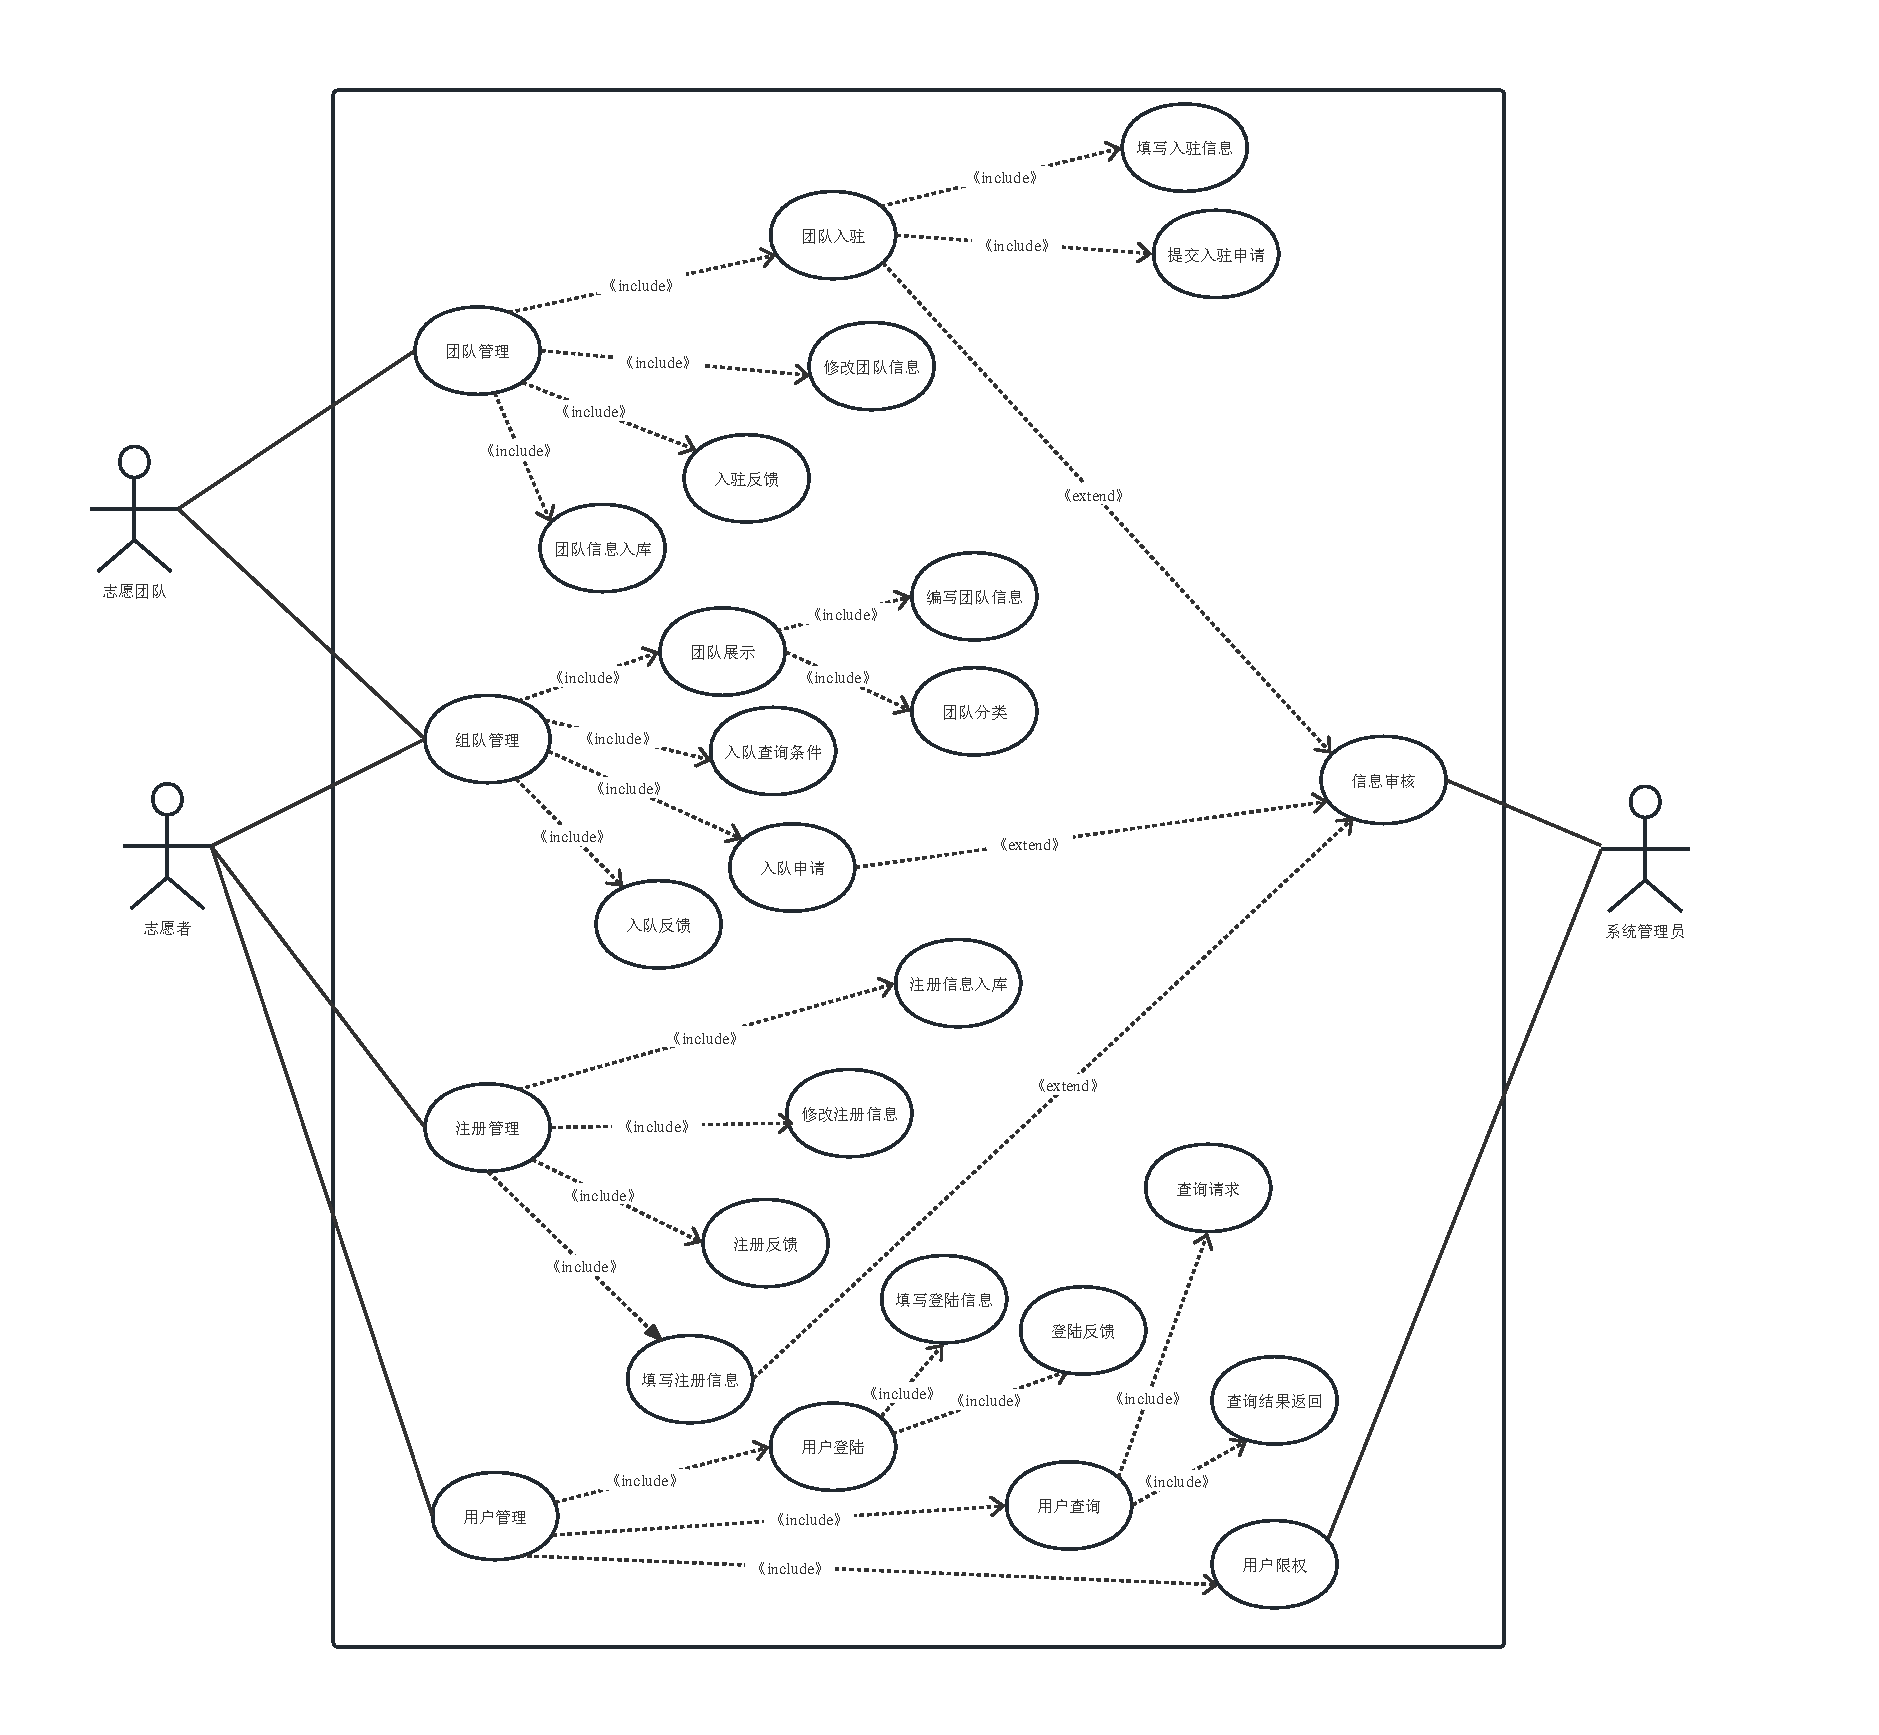
\includegraphics[scale=0.5]{OOA/fig/1-信息管理/信息管理用况图.pdf}} 
    \bicaption{Volunet信息管理系统用况图}{Information Management System Usage Chart of Volunet} 
\end{figure}


\subsubsection{志愿服务系统}
\begin{figure}[H] 
    \center{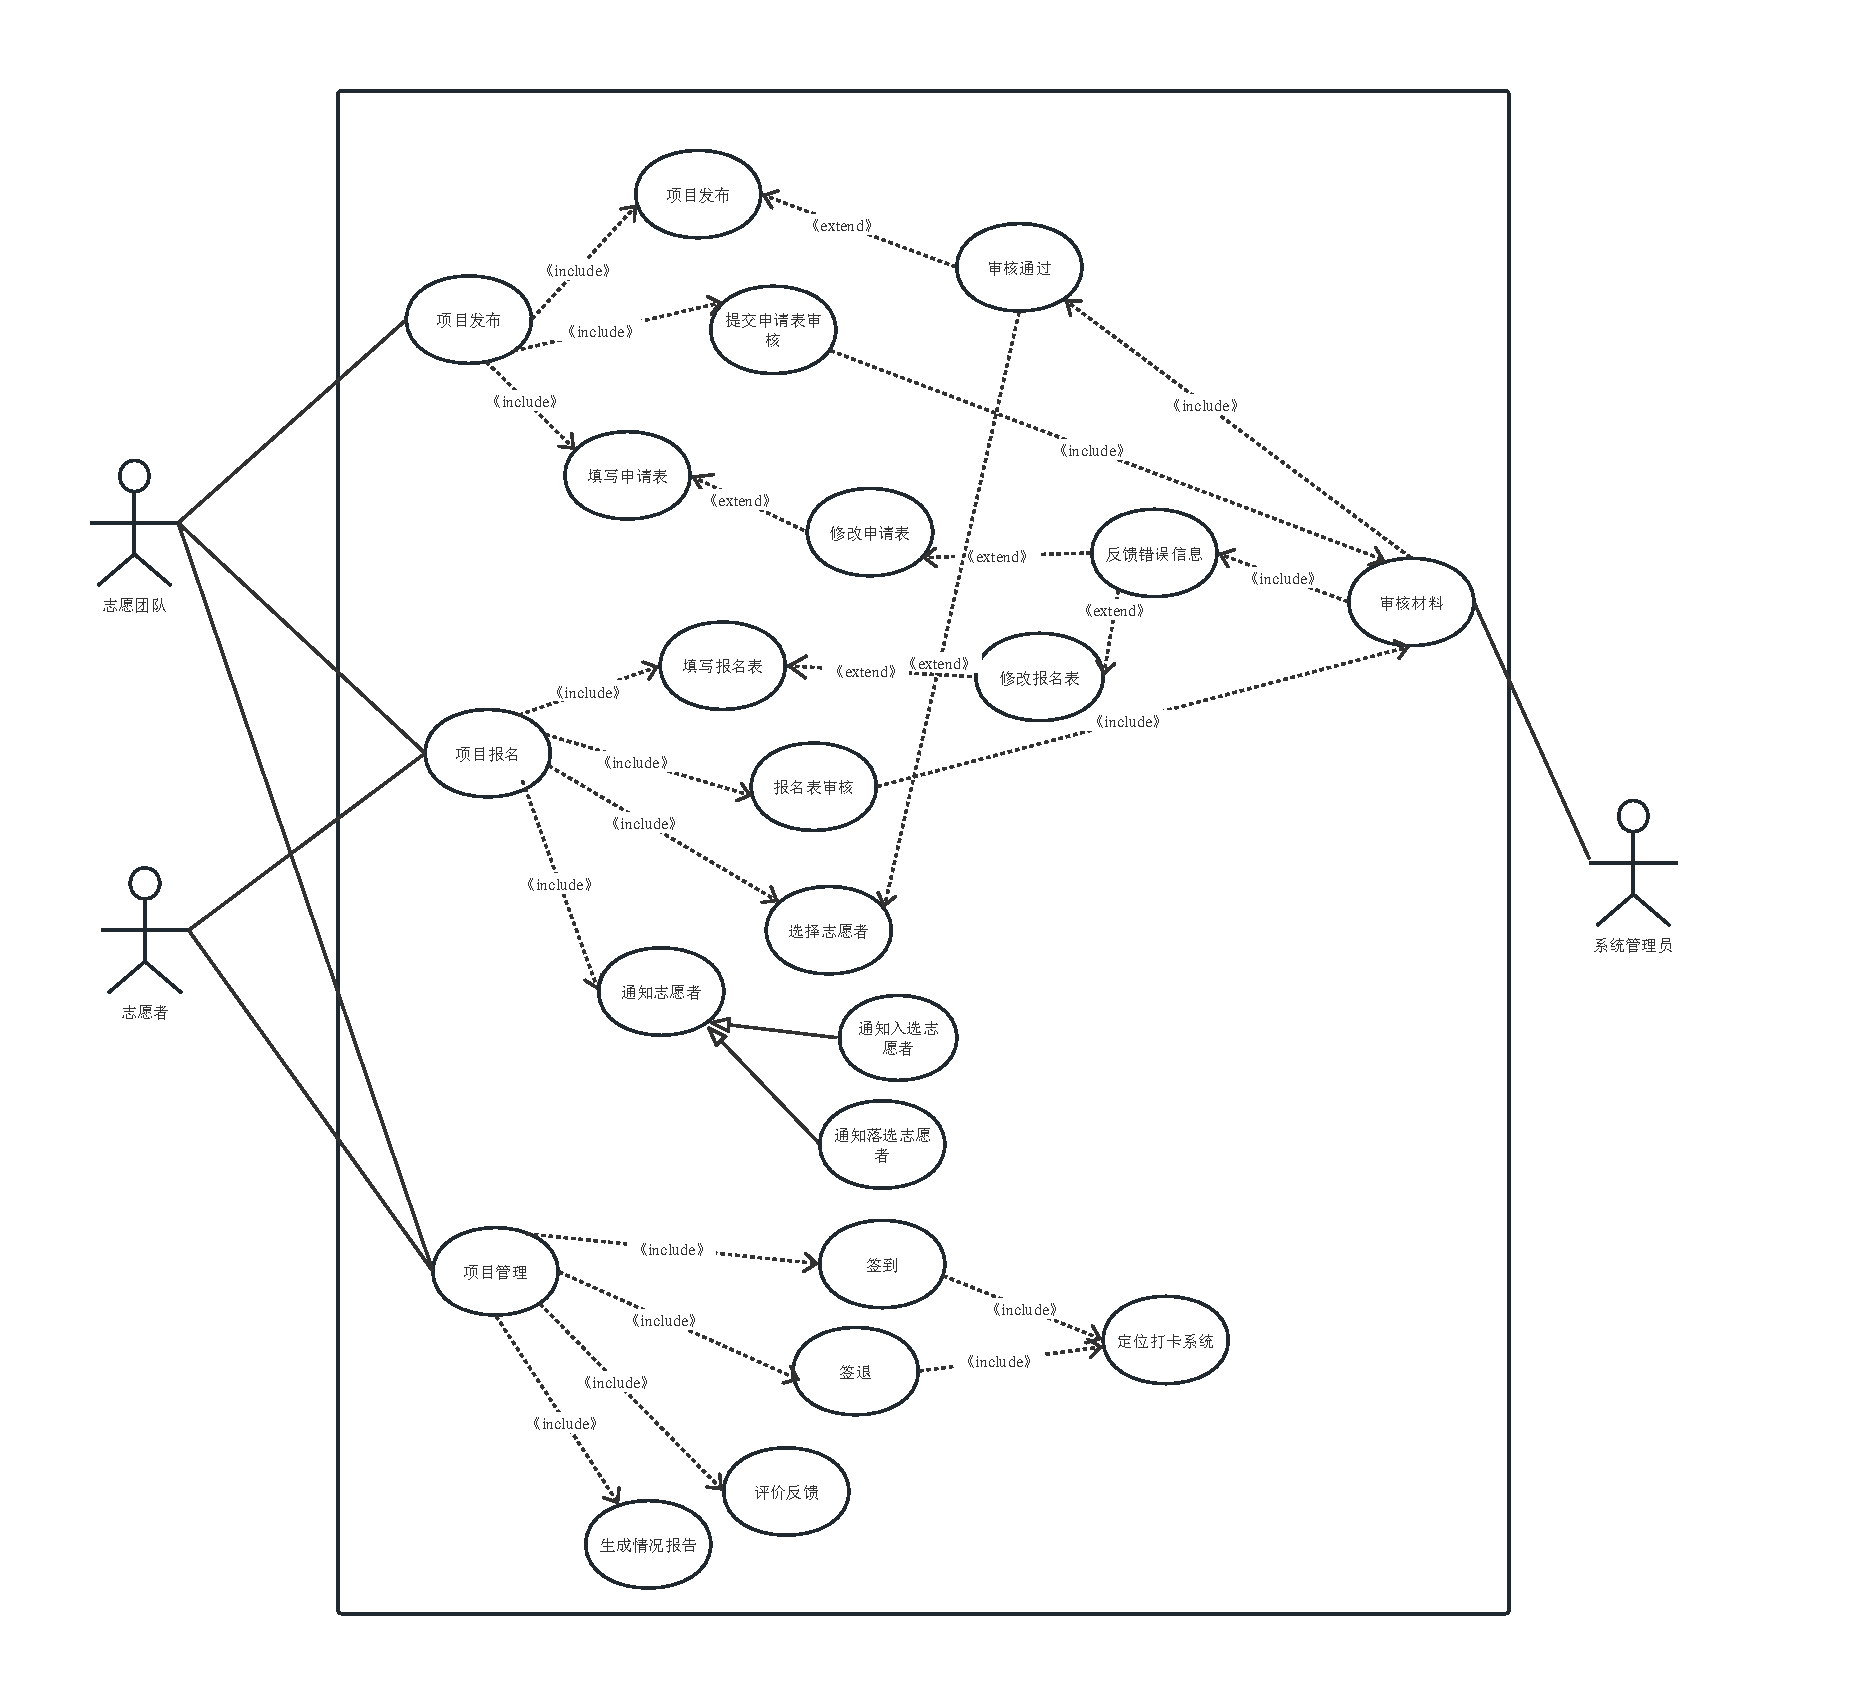
\includegraphics[scale=0.5]{OOA/fig/2-志愿服务/VS-用况图.pdf}} 
    \bicaption{Volunet志愿服务系统用况图}{Voluntary Service System Usage Chart of Volunet} 
\end{figure}


\subsubsection{爱心捐助系统}
\begin{figure}[H] 

    \center{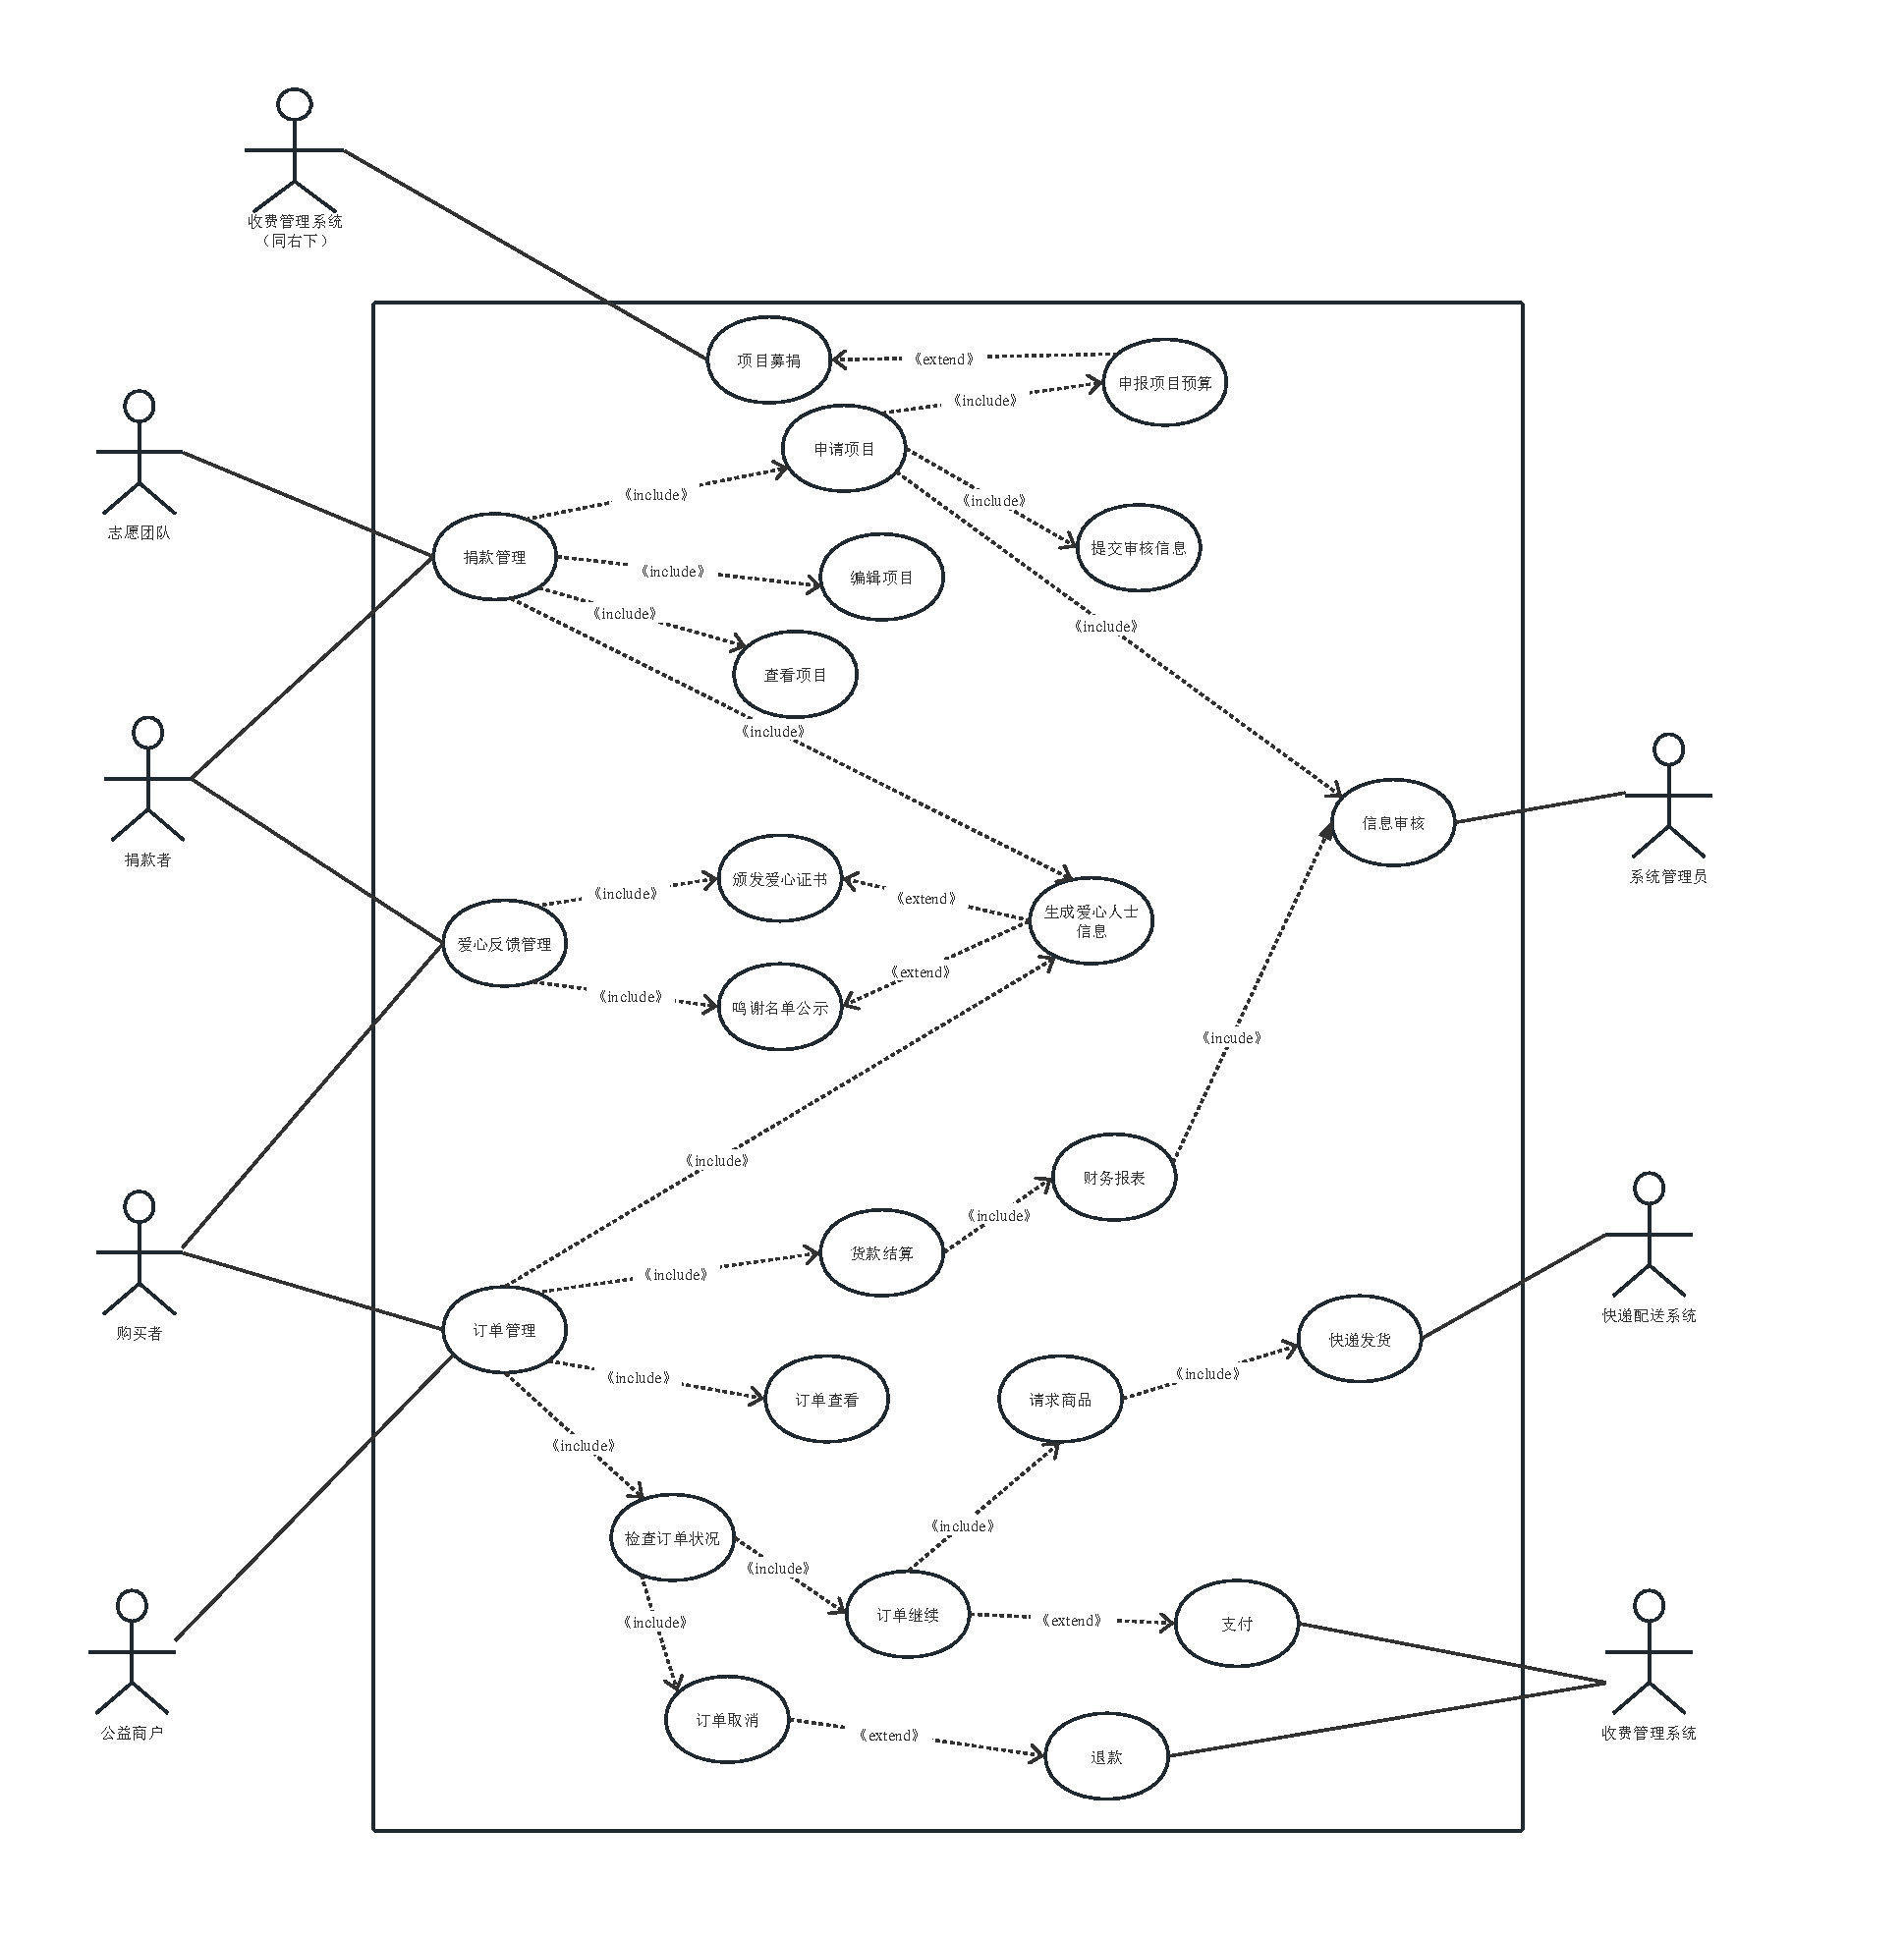
\includegraphics[scale=0.5]{OOA/fig/3-爱心管理/爱心管理用况图.pdf}} 
    \bicaption{Volunet爱心捐助系统用况图}{Love Donation System Usage Chart of Volunet} 
\end{figure}

\subsubsection{公益课程系统}
\begin{figure}[H] 

    \center{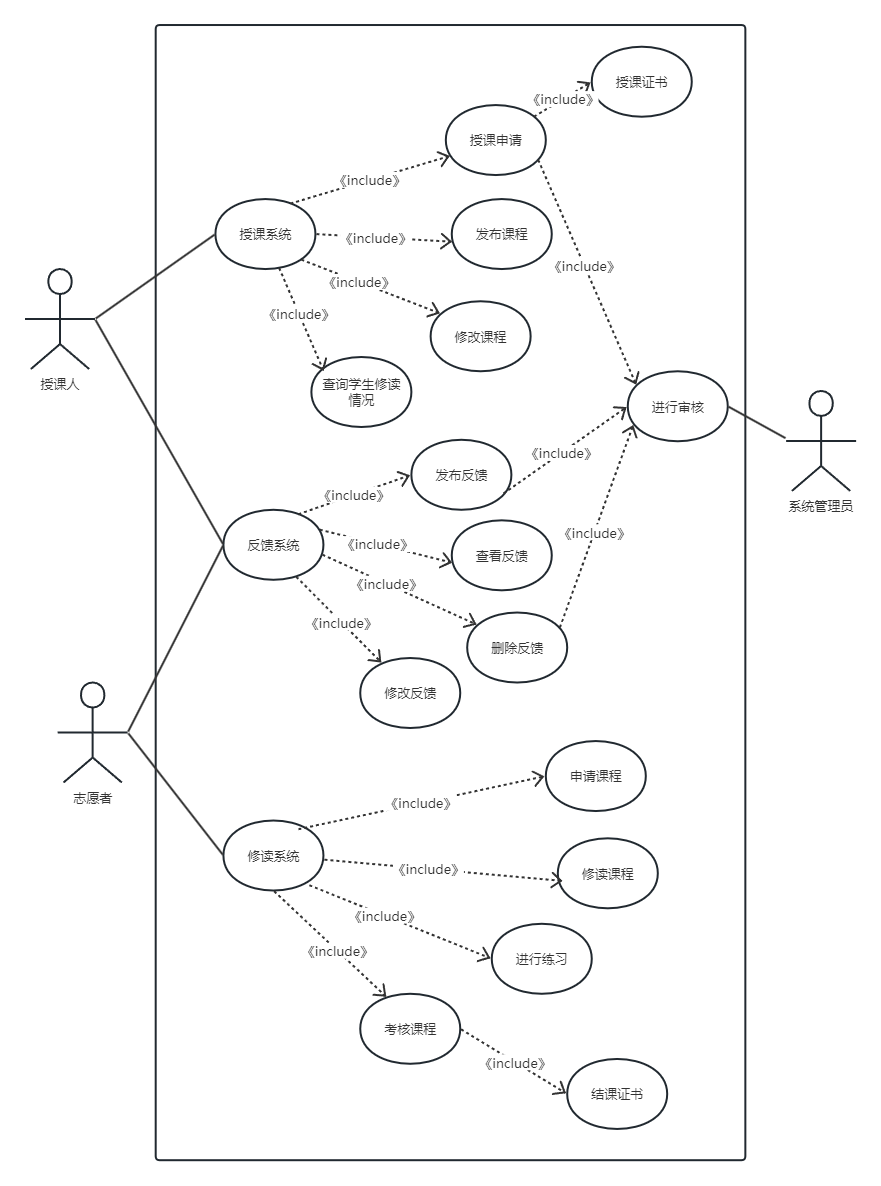
\includegraphics[scale=0.42]{OOA/fig/4-课程管理/课程管理用况图.png}} 
    \bicaption{Volunet公益课程系统用况图}{Course System Usage Chart of Volunet} 
\end{figure}

\subsubsection{交流论坛系统}
\begin{figure}[H] 

    \center{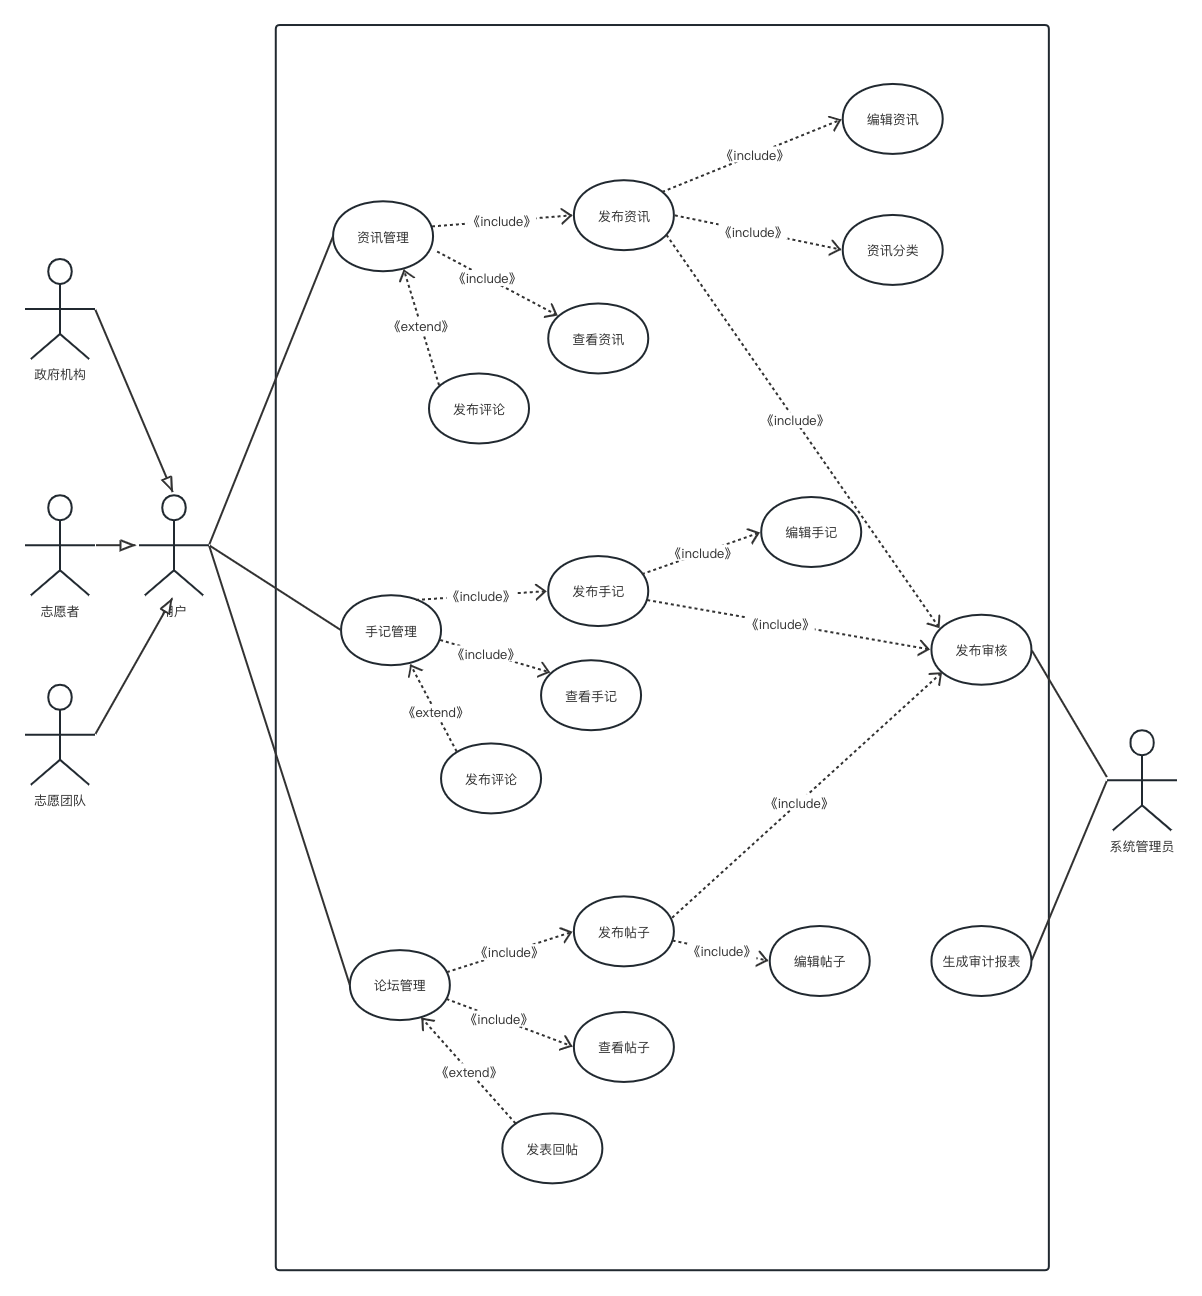
\includegraphics[scale=0.35]{OOA/fig/5-论坛管理/论坛管理用况图.png}} 
    \bicaption{Volunet交流论坛系统用况图}{Communication System Use Case Chart of Volunet} 
\end{figure}

\subsubsection{志愿交友系统}
\begin{figure}[H] 

    \center{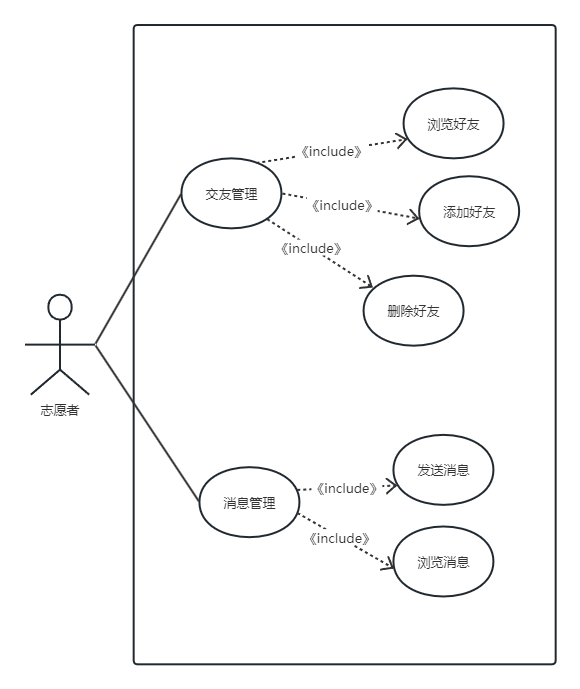
\includegraphics[scale=0.5]{OOA/fig/6-交友管理/志愿交友管理用况图.png}} 
    \bicaption{Volunet志愿交友用况图}{Volunteer Friends System Usage Chart of Volunet} 
\end{figure}

\subsection{用况描述}

\subsubsection{信息管理系统}

信息管理系统的用况描述如下:

\begin{framed}
\noindent
用况名称:用户管理\\
参与的执行者:志愿者、系统管理员\\
前置条件:用户身份为志愿者,且已经合法登陆到这个系统\\
事件流:\\
基本路径:
\begin{enumerate}[itemsep=2pt,topsep=0pt,parsep=0pt,itemindent=1em]
    \item 当志愿者进入到用户页面时,用况开始
    \item 志愿团队进行页面选择并发出操作指令
    \item 系统对志愿者的操作进行处理:
    \begin{enumerate}[itemsep=2pt,topsep=0pt,parsep=0pt,itemindent=1em]
          \item 用户主页编辑:若有权限则继续执行;否则退回到上一步
          \item 用户查找:继续执行第8步
      \end{enumerate}
    \item 志愿者进入主页编写界面
    \item 志愿者获取展示列表
    \item 志愿者按需编辑主页标题、图片和展示列表
    \item 志愿者编辑完成可预览用户主页,点击确认后提示用户主页成功更新,用况结束
    \item 志愿者浏览用户主页列表
    \item 志愿者选择搜索框并按条件查询
    \item 展示志愿者查询结果,用况结束
\end{enumerate}
\noindent
可选路径:\par
    在选择提交主页编辑之前的任何时间,志愿团队可以退出该系统,系统会自动保存当前历史记录,并在下一次进入系统时询问是否恢复\\
后置条件:用户编辑好后的主页会进行更新,替代之前的信息
\end{framed}

\begin{framed}
\noindent
用况名称:注册管理\\
参与的执行者:志愿者、系统管理员\\
前置条件:志愿者需要访问注册页面,系统管理员需要具有管理注册信息的权限,二者均已合法登陆到这个系统\\
事件流:\\
基本路径:
\begin{enumerate}[itemsep=2pt,topsep=0pt,parsep=0pt,itemindent=1em]
   \item 志愿者填写必要的信息,如用户名、密码、电子邮件地址等\item 志愿者点击“注册”按钮
   \item 系统管理员验证用户提供的信息是否有效
   \item 如果验证通过,系统将用户的信息保存到数据库中,并向志愿者发送确认邮件
   \item 志愿者收到确认邮件并点击其中的链接以激活账户 
   \item 志愿者账户激活成功,志愿者可以登录系统
\end{enumerate}
\noindent
可选路径:\par
     \begin{enumerate}[itemsep=2pt,topsep=0pt,parsep=0pt,itemindent=1em] \item 如果用户提供的信息无效,系统将显示错误消息并要求用户更正
     \item 如果用户没有收到确认邮件,用户可以请求系统重新发送 
     \end{enumerate} 
后置条件:用户账户已成功注册并激活,用户可以登录系统
\end{framed}

\begin{framed}
\noindent
用况名称:组队管理\\
参与的执行者:志愿者、志愿团队、系统管理员\\
前置条件:志愿者已经注册并登录到系统中;志愿团队已经创建并发布了一个活动\\
事件流:\\
基本路径: \begin{enumerate}[itemsep=2pt,topsep=0pt,parsep=0pt,itemindent=1em] \item 志愿者在系统中查看到志愿团队发布的活动,并决定加入该活动的团队 \item 志愿者向志愿团队发送加入请求 \item 志愿团队收到请求后,审核志愿者的信息并决定是否接受该志愿者 \item 如果志愿团队接受了志愿者的请求,系统将志愿者加入该团队,并将该团队的信息显示在志愿者的个人主页上 \end{enumerate}
\noindent
可选路径:\par
     如果志愿团队拒绝了志愿者的请求,系统将不会将志愿者加入该团队,并给志愿者发送拒绝信息 \\
后置条件:志愿者已经加入了志愿团队,并可以参加该团队发布的活动

\end{framed}

\begin{framed}
\noindent
用况名称:团队管理\\
参与的执行者:志愿团队、系统管理员\\
前置条件:志愿团队已经注册并登录到系统中,且系统管理员已经授权志愿团队进行团队管理\\
事件流:\\
基本路径:
\begin{enumerate}[itemsep=2pt,topsep=0pt,parsep=0pt,itemindent=1em] \item 志愿团队登录到系统中 \item 在系统中选择团队管理功能。 \item 在团队管理页面中,可以进行以下操作: \begin{enumerate}[itemsep=2pt,topsep=0pt,parsep=0pt,itemindent=1em] \item 添加或删除团队成员 \item 分配任务给团队成员。 \item 查看团队成员的任务进度 \item 编辑团队成员的个人信息 \item 禁止或允许团队成员访问系统\end{enumerate} 
\end{enumerate}
\noindent
可选路径: \par
 \begin{enumerate}[itemsep=2pt,topsep=0pt,parsep=0pt,itemindent=1em]  \item 在团队管理页面中,如果志愿团队没有权限进行某些操作,系统会提示“权限不足”的错误信息 \item 如果团队成员的个人信息不完整或错误,系统管理员可以要求团队成员进行修改  \end{enumerate} 
后置条件:团队成员的任务分配和进度记录已经更新到系统中;团队成员的个人信息已经保存到系统中

\end{framed}

\begin{framed}
\noindent
用况名称:信息审核\\
参与的执行者:系统管理员\\
前置条件:系统中存在需要审核的信息,且系统管理员已经合法登陆到这个系统
事件流: \begin{enumerate}[itemsep=2pt,topsep=0pt,parsep=0pt,itemindent=1em] \item 系统管理员登录审核系统 \item 系统管理员选择需要审核的信息 \item 系统管理员查看信息内容,判断是否符合审核标准 \item 如果信息符合审核标准,系统管理员将信息标记为“审核通过”,并记录审核结果 \item 如果信息不符合审核标准,系统管理员将信息标记为“审核不通过”,并记录审核结果 \end{enumerate}
\noindent
可选路径: \par
在步骤3中,如果系统管理员无法判断信息是否符合审核标准,可以将信息标记为“待定”,并将信息转交给其他审核人员审核\\
后置条件:审核结果被记录在系统中,审核完成

\end{framed}

\subsubsection{志愿服务系统}
志愿服务系统的用况描述如下:
\begin{framed}
\noindent
用况名称:项目发布\\
参与的执行者:志愿团队、系统管理员\\
前置条件:用户身份为志愿团队,且通过资质审核可以提交志愿项目发布申请\\
事件流:\\
基本路径:
\begin{enumerate}[itemsep=2pt,topsep=0pt,parsep=0pt,itemindent=1em]
    \item 当志愿团队新建志愿项目单时,用况开始
    \item 志愿团队填写志愿项目信息
    \item 志愿团队提交志愿项目申请单
    \item 系统管理员对提交的志愿项目进行审核:
    \begin{enumerate}[itemsep=2pt,topsep=0pt,parsep=0pt,itemindent=1em]
          \item 审核通过:项目发布,用况结束
          \item 审核失败:将错误信息反馈给志愿团队,转到2继续
      \end{enumerate}
\end{enumerate}
\noindent
可选路径:\par
    在选择提交志愿项目申请单之前的任何时间,志愿团队可以退出该系统,系统会自动保存当前历史记录,并在下一次进入系统时询问是否恢复\\
后置条件:项目通过审核并发布在Volunet,该项目会被编号进入志愿项目库

\end{framed}

\begin{framed} \noindent 用况名称:项目报名\\ 
参与的执行者:志愿者、志愿团队、系统管理员\\
前置条件:志愿者已经注册并登录系统\\ 
事件流:\\
基本路径: \begin{enumerate}[itemsep=2pt,topsep=0pt,parsep=0pt,itemindent=1em] \item 志愿者进入项目报名页面。 \item 系统显示可报名的项目列表。 \item 志愿者选择感兴趣的项目。 \item 系统显示该项目的详细信息和报名表格。 \item 志愿者填写报名表格并提交。 \item 系统保存志愿者的报名信息,并将其加入该项目的报名名单中。 \item 系统向志愿者发送报名成功的通知。 \end{enumerate} \noindent 
可选路径: \par
如果该项目已经满员,系统提示志愿者该项目已经无法报名,返回步骤2。如果志愿者填写的报名表格信息不完整或不符合要求,系统提示志愿者修改并重新提交,返回步骤4。 \\
 \end{framed}

 \begin{framed} \noindent 
用况名称:项目管理\\ 
参与的执行者:志愿者、志愿团队、系统管理员\\
 前置条件:项目需求已经明确并且项目计划已经制定\\
 事件流: \\
基本路径: \begin{enumerate}[itemsep=2pt,topsep=0pt,parsep=0pt,itemindent=1em] \item 系统管理员创建项目。 \item 系统管理员指派志愿者和志愿团队成员。 \item 志愿者和志愿团队成员接受任务并开始执行。 \item 志愿者和志愿团队成员定期向系统管理员报告项目进展情况。 \item 系统管理员根据报告情况对项目进度进行监控和管理。 \item 当项目完成时,系统管理员关闭项目并将成果提交给相关方。 \end{enumerate} 
可选路径: \par 
如果项目进展不如预期,系统管理员可以采取措施来加速项目进度。如果项目需求发生变化,系统管理员可以更新项目计划并通知相关人员\\
\end{framed}




\subsubsection{爱心捐助系统}

爱心捐助系统的用况描述如下:

\begin{framed}
\noindent
用况名称:捐款管理\\
参与的执行者:捐款者、志愿团队、系统管理员\\
前置条件:用户身份为志愿团队,且通过资质审核可以提交志愿项目发布申请;用户身份为捐款者,且已经合法登陆到这个系统\\
事件流:\\
基本路径:
\begin{enumerate}[itemsep=2pt,topsep=0pt,parsep=0pt,itemindent=1em]
    \item 当志愿团队新建资助项目单时,用况开始
    \item 志愿团队填写资助项目信息
    \item 志愿团队提交资助项目申请单
    \item 系统管理员对提交的信息进行审核:
    \begin{enumerate}[itemsep=2pt,topsep=0pt,parsep=0pt,itemindent=1em]
          \item 审核通过:项目发布,志愿团队相关用况结束
          \item 审核失败:将错误信息反馈给志愿团队,转到2继续
      \end{enumerate}
    \item 当捐款者选择募捐项目时,用况开始
    \item 捐款者为选择的项目输入捐款的数额
    \item 捐款者选择支付方式并进行支付
    \item 系统检验支付是否成功,如果捐款者账户的余额不足以支付,系统将提示用户支付失败并重新尝试
    \item 当支付成功后,捐款就被标记上已经支付,同时记录捐款者信息用于爱心反馈,捐款者相关用况结束
\end{enumerate}
\noindent
可选路径:\par
     \begin{enumerate}[itemsep=2pt,topsep=0pt,parsep=0pt,itemindent=1em]  \item 在选择提交资助项目申请单之前的任何时间,志愿团队可以退出该系统,系统会自动保存当前历史记录,并在下一次进入系统时询问是否恢复 \item 在支付开始之前的任何时间,捐款者可以退出该系统,系统会自动保存当前历史记录,并在下一次进入系统时询问是否恢复  \end{enumerate} 
后置条件:资助项目通过审核并添加进募捐项目列表,捐款者支付成功后的信息会保存在系统中并做标记
\end{framed}

\begin{framed}
\noindent
用况名称:订单管理\\
参与的执行者:购买者、爱心商户、系统管理员\\
前置条件:用户身份为爱心商户,且营业状态正常;用户身份为购买者,且已经合法登陆到这个系统\\
事件流:\\
基本路径:
\begin{enumerate}[itemsep=2pt,topsep=0pt,parsep=0pt,itemindent=1em]
    \item 当公益商户添加公益商品时,用况开始
    \item 公益商户填写公益商品信息
    \item 公益商户提交公益商品上架单
    \item 系统管理员对提交的商品信息进行审核:
    \begin{enumerate}[itemsep=2pt,topsep=0pt,parsep=0pt,itemindent=1em]
          \item 审核通过:商品发布,公益商户相关用况结束
          \item 审核失败:将失败信息反馈给公益商户,转到2继续
      \end{enumerate}
    \item 当购买者选择公益商品时,用况开始
    \item 购买者将选择的公益商品加入购物车并提交订单
    \item 购买者选择支付方式并进行支付
    \item 系统检验支付是否成功,如果捐款者账户的余额不足以支付,系统将提示用户支付失败并重新尝试
    \item 当支付成功后,订单就被标记上已经支付
    \item 支付完成的订单将接入快递配送平台进行配送
    \item 购买者收到货物后对订单进行签收
    \item 订单完结,同时记录购买者信息用于爱心反馈,购买者相关用况结束
\end{enumerate}
\noindent
可选路径:\par
         \begin{enumerate}[itemsep=2pt,topsep=0pt,parsep=0pt,itemindent=1em]  \item 在选择提交公益商品信息之前的任何时间,公益商户可以退出该系统,系统会自动保存当前历史记录,并在下一次进入系统时询问是否恢复 \item 在用况开始到支付开始之前以及支付完成之后的任何时间,购买者可以退出该系统,系统会自动保存当前历史记录,并在下一次进入系统时询问是否恢复  \end{enumerate} 
后置条件:公益商品通过审核并添加进商品页面,购买者订单完成后的信息会保存在系统中并做标记
\end{framed}

\begin{framed}
\noindent
用况名称:爱心反馈管理\\
参与的执行者:捐款者、购买者\\
前置条件:用户身份为爱心人士(即捐款者和购买者),且已经合法登陆到这个系统\\
事件流:\\
基本路径:
\begin{enumerate}[itemsep=2pt,topsep=0pt,parsep=0pt,itemindent=1em]
    \item 当爱心人士查看爱心反馈页面时,用况开始
    \item 爱心人士选择查看内容:
    \begin{enumerate}[itemsep=2pt,topsep=0pt,parsep=0pt,itemindent=1em]
          \item 查看爱心证书:显示其对应的爱心证书,用况结束
          \item 查看鸣谢名单:显示公示的鸣谢爱心人士名单,用况结束
      \end{enumerate}
\end{enumerate}
\noindent
可选路径:\par
    在任何时间,爱心人士可以退出该系统,系统会自动保存当前历史记录,并在下一次进入系统时询问是否恢复\\
后置条件:无

\end{framed}

\begin{framed}
\noindent
用况名称:信息审核\\
参与的执行者:系统管理员\\
前置条件:系统中存在需要审核的信息,且系统管理员已经合法登陆到这个系统
事件流: \begin{enumerate}[itemsep=2pt,topsep=0pt,parsep=0pt,itemindent=1em] \item 系统管理员登录审核系统 \item 系统管理员选择需要审核的信息 \item 系统管理员查看信息内容,判断是否符合审核标准 \item 如果信息符合审核标准,系统管理员将信息标记为“审核通过”,并记录审核结果 \item 如果信息不符合审核标准,系统管理员将信息标记为“审核不通过”,并记录审核结果 \end{enumerate}
\noindent
可选路径: \par
在步骤3中,如果系统管理员无法判断信息是否符合审核标准,可以将信息标记为“待定”,并将信息转交给其他审核人员审核\\
后置条件:审核结果被记录在系统中,审核完成

\end{framed}

\subsubsection{公益课程系统}

公益课程系统的用况描述如下:

\begin{framed}
\noindent
用况名称:授课管理\\
参与的执行者:授课人、系统管理员\\
前置条件:用户身份为状态无异常账号,且通过资质审核可以提交课程项目发布申请;用户身份为系统管理员,且已经合法登陆到这个系统\\
事件流:\\
基本路径:
\begin{enumerate}[itemsep=2pt,topsep=0pt,parsep=0pt,itemindent=1em]
    \item 当用户新创建授课申请单时,用况开始
    \item 用户填写授课申请单信息
    \item 用户提交授课申请单
    \item 系统管理员对提交的信息进行审核:
    \begin{enumerate}[itemsep=2pt,topsep=0pt,parsep=0pt,itemindent=1em]
          \item 审核通过:资质核验通过发布,用户获得授课资格,成为授课人
          \item 审核失败:将核验信息反馈给授课人,转到2继续
      \end{enumerate}
    \item 当授课人选择创建课程时,用况开始
    \item 授课人为创建的课程输入必要的信息
    \item 授课人选择为创建的课程导入必要的课程资料
    \item 授课进行发布课程,在课程首页可以获得展示
\end{enumerate}
\noindent
可选路径:\par
     \begin{enumerate}[itemsep=2pt,topsep=0pt,parsep=0pt,itemindent=1em]  \item 系统管理员将授课人分配到不同的课程中,进行管理和监督教学工作。 \item 授课人创建考试和评估任务,对学生进行考核和评估。  \end{enumerate} 
后置条件:授课人完成课程的上课记录,系统需要自动计算学生的考勤情况并更新到学生的考勤记录中
\end{framed}

\begin{framed}
\noindent
用况名称:修读管理\\
参与的执行者:授课人、志愿者、系统管理员\\
前置条件:用户身份为授课人,且资质状态正常;用户身份为志愿者,且已经合法登陆到这个系统\\
事件流:\\
基本路径:
\begin{enumerate}[itemsep=2pt,topsep=0pt,parsep=0pt,itemindent=1em]
    \item 当志愿者选择查看课程时,用况开始
    \item 志愿者选择查看具体课程信息
    \item 志愿者提交选课申请
    \item 系统管理员对提交的选课申请信息进行审核:
    \begin{enumerate}[itemsep=2pt,topsep=0pt,parsep=0pt,itemindent=1em]
          \item 审核通过:课程选择成功,志愿者成为此课程学生
          \item 审核失败:将失败信息反馈给志愿者,转到2继续
      \end{enumerate}
    \item 当志愿者购买课程时,用况开始
    \item 志愿者将选择的课程加入购物车并提交订单
    \item 志愿者选择支付方式并进行支付
    \item 系统检验支付是否成功,如果志愿者账户的余额不足以支付,系统将提示志愿者支付失败并重新尝试
    \item 当支付成功后,订单就被标记上已经支付
    \item 当前订单的课程向此志愿者进行解锁
    \item 志愿者可以对课程进行学习、并与授课人交流提问
    \item 课程完结,同时记录志愿者信息用于课程反馈,志愿者相关用况结束
\end{enumerate}
\noindent
可选路径:\par
         \begin{enumerate}[itemsep=2pt,topsep=0pt,parsep=0pt,itemindent=1em]  \item 在选择提交课程之前的任何时间,志愿者可以退出该系统,系统会自动保存当前历史记录,并在下一次进入系统时询问是否恢复 
         \item 在用况开始到支付开始之前以及支付完成之后的任何时间,志愿者可以退出该系统,系统会自动保存当前历史记录,并在下一次进入系统时询问是否恢复  \end{enumerate} 
后置条件:完成一定的课程和通过相关考试后,提供相关结课证书
\end{framed}

\begin{framed}
\noindent
用况名称:反馈管理\\
参与的执行者:志愿者、系统管理员、授课人\\
前置条件:用户身份为志愿者、系统管理员或授课人,且已经合法登陆到这个系统\\
事件流:\\
基本路径:
\begin{enumerate}[itemsep=2pt,topsep=0pt,parsep=0pt,itemindent=1em]
    \item 当志愿者选择课程反馈界面时,用况开始
    \item 志愿者选择撰写课程反馈界面
    \item 志愿者提交课程反馈
    \item 系统管理员对提交的反馈信息进行审核:
    \begin{enumerate}[itemsep=2pt,topsep=0pt,parsep=0pt,itemindent=1em]
          \item 审核通过:课程反馈发布成功,志愿者用况结束
          \item 审核失败:将审核失败信息反馈给志愿者,转到2继续
      \end{enumerate}
    \item 当授课人查看课程反馈页面时,用况开始
    \item 授课人选择查看内容:
    \begin{enumerate}[itemsep=2pt,topsep=0pt,parsep=0pt,itemindent=1em]
          \item 查看学生修读情况:显示其对应的修读情况,用况结束
          \item 查看课程反馈:显示提交的课程反馈,用况结束
      \end{enumerate}
\end{enumerate}
\noindent
可选路径:\par
         \begin{enumerate}[itemsep=2pt,topsep=0pt,parsep=0pt,itemindent=1em]  \item 在任何时间,用户可以退出该系统,系统会自动保存当前历史记录,并在下一次进入系统时询问是否恢复 
         \item 如果系统管理员无法判断反馈信息是否符合审核标准,可以将信息标记为“待定”,并将信息转交给其他审核人员审核  \end{enumerate}
后置条件:反馈结果被记录在系统中,反馈完成

\end{framed}


\subsubsection{交流论坛系统}

交流论坛系统的用况描述如下:
\begin{framed}
\noindent
用况名称:资讯管理\\
参与的执行者:用户\\
前置条件:一个合法的用户已经登录到了这个系统\\
事件流:\\
基本路径:
\begin{enumerate}[itemsep=2pt,topsep=0pt,parsep=0pt,itemindent=1em]
    \item 用户通过身份验证进入资讯管理系统,用况开始
    \item 用户点击“资讯管理”按钮
    \item 进入资讯管理主界面
    \item 显示资讯目录
    \item 当用户点击查看资讯时以任意次数和合理的次序重复如下事件流,直至出现创建资讯事件流
    \begin{enumerate}[itemsep=2pt,topsep=0pt,parsep=0pt,itemindent=1em]
          \item 系统展示资讯
          \item 用户评论资讯
      \end{enumerate}
    \item 用户选择发布资讯
    \item 以任意次数和合理的次序重复如下事件流,直至出现发布事件流
    \begin{enumerate}[itemsep=2pt,topsep=0pt,parsep=0pt,itemindent=1em]
          \item 编辑资讯
          \item 资讯分类
          \item 发布审核
      \end{enumerate}
    \item 发布资讯或退出
        \begin{enumerate}[itemsep=2pt,topsep=0pt,parsep=0pt,itemindent=1em]
          \item 发布资讯
          \item 退出资讯管理
      \end{enumerate}
\end{enumerate}
\noindent
可选路径:\par
   \begin{enumerate}[itemsep=2pt,topsep=0pt,parsep=0pt,itemindent=1em]  \item 在选择发布资讯前的任何时候,用户都可以退出系统,待发布的资讯作为草稿保存 \item 在基本路径的第$5$步,如果有任何不合法的信息,系统提示用户去修改这些信息\item 在基本路径的第$7$步,如果有任何不合法的信息,系统提示用户去修改这些信息  \end{enumerate} 
后置条件:如果用户提交成功,资讯管理系统会执行相关操作;否则,维持不变
\end{framed}

\begin{framed}
\noindent
用况名称:发布资讯\\
参与的执行者:用户\\
前置条件:成功登录到资讯管理主页面\\
事件流:\\
基本路径:
\begin{enumerate}[itemsep=2pt,topsep=0pt,parsep=0pt,itemindent=1em]
     \item 选择待发布的资讯
     \item 发布资讯
\end{enumerate}
\noindent
后置条件:资讯
\end{framed}


\begin{framed}
\noindent
用况名称:编辑资讯\\
参与的执行者:用户\\
前置条件:成功登录到资讯管理主页面\\
事件流:\\
基本路径:
\begin{enumerate}[itemsep=2pt,topsep=0pt,parsep=0pt,itemindent=1em]
    \item 用户点击资讯
    \item 用户点击写资讯
    \item 转到文章编辑页面,输入标题或正文
    \begin{enumerate}[itemsep=2pt,topsep=0pt,parsep=0pt,itemindent=1em]
          \item 发布刚刚编辑的资讯
          \item 存为草稿或私人文章 
      \end{enumerate}
\end{enumerate}
\noindent
后置条件:资讯
\end{framed}

\begin{framed}
\noindent
用况名称:资讯分类\\
参与的执行者:用户\\
前置条件:成功登录到资讯管理主页面\\
事件流:\\
基本路径:
\begin{enumerate}[itemsep=2pt,topsep=0pt,parsep=0pt,itemindent=1em]
    \item 用户点击资讯
    \item 用户点击写资讯
    \item 转到文章编辑页面,输入标题或正文
    \begin{enumerate}[itemsep=2pt,topsep=0pt,parsep=0pt,itemindent=1em]
          \item 发布刚刚编辑的资讯
          \item 存为草稿或私人文章 
      \end{enumerate}
\end{enumerate}
\noindent
后置条件:资讯
\end{framed}

\begin{framed}
\noindent
用况名称:查看资讯\\
参与的执行者:用户\\
前置条件:成功登录到资讯管理主页面\\
事件流:\\
基本路径:
\begin{enumerate}[itemsep=2pt,topsep=0pt,parsep=0pt,itemindent=1em]
    \item 用户点击资讯
    \item 查看所有资讯
    \begin{enumerate}[itemsep=2pt,topsep=0pt,parsep=0pt,itemindent=1em]
          \item 按资讯分类查看
          \item 按资讯归档查看
      \end{enumerate}
\end{enumerate}
\noindent
后置条件:查看之前发表过的资讯或草稿
\end{framed}

\begin{framed}
\noindent
用况名称:资讯评论\\
参与的执行者:用户\\
前置条件:成功登录到资讯管理主页面\\
事件流:\\
基本路径:
\begin{enumerate}[itemsep=2pt,topsep=0pt,parsep=0pt,itemindent=1em]
    \item 用户点击资讯
    \item 查看所有资讯
    \item 选择资讯点击评论
    \item 编辑资讯评论正文
    \item 选择提交评论
    \end{enumerate}
\noindent
后置条件:资讯评论成功
\end{framed}

\begin{framed}
\noindent
用况名称:手记管理\\
参与的执行者:用户\\
前置条件:一个合法的用户已经登录到了这个系统\\
事件流:\\
基本路径:
\begin{enumerate}[itemsep=2pt,topsep=0pt,parsep=0pt,itemindent=1em]
    \item 用户通过身份验证进入手记管理系统,用况开始
    \item 用户点击“手记管理”按钮
    \item 进入手记管理主界面
    \item 显示手记目录
    \item 当用户点击查看手记时以任意次数和合理的次序重复如下事件流,直至出现创建手记事件流
    \begin{enumerate}[itemsep=2pt,topsep=0pt,parsep=0pt,itemindent=1em]
          \item 系统展示手记
          \item 用户评论手记
      \end{enumerate}
    \item 用户选择发布手记
    \item 以任意次数和合理的次序重复如下事件流,直至出现发布事件流
    \begin{enumerate}[itemsep=2pt,topsep=0pt,parsep=0pt,itemindent=1em]
          \item 编辑手记
          \item 发布审核
      \end{enumerate}
    \item 发布手记或退出
        \begin{enumerate}[itemsep=2pt,topsep=0pt,parsep=0pt,itemindent=1em]
          \item 发布手记
          \item 退出手记管理
      \end{enumerate}
\end{enumerate}
\noindent
可选路径:\par
   \begin{enumerate}[itemsep=2pt,topsep=0pt,parsep=0pt,itemindent=1em]  \item 在选择发布手记前的任何时候,用户都可以退出系统,待发布的手记作为草稿保存 \item 在基本路径的第$5$步,如果有任何不合法的信息,系统提示用户去修改这些信息\item 在基本路径的第$7$步,如果有任何不合法的信息,系统提示用户去修改这些信息  \end{enumerate} 
后置条件:如果用户提交成功,手记管理系统会执行相关操作;否则,维持不变
\end{framed}

\begin{framed}
\noindent
用况名称:发布手记\\
参与的执行者:用户\\
前置条件:成功登录到手记管理主页面\\
事件流:\\
基本路径:
\begin{enumerate}[itemsep=2pt,topsep=0pt,parsep=0pt,itemindent=1em]
    \item 选择待发布的手记
    \item 发布手记
\end{enumerate}
\noindent
后置条件:发表编辑好的手记,或者存问草稿或私人手记
\end{framed}

\begin{framed}
\noindent
用况名称:编辑手记\\
参与的执行者:用户\\
前置条件:成功登录到资讯管理主页面\\
事件流:\\
基本路径:
\begin{enumerate}[itemsep=2pt,topsep=0pt,parsep=0pt,itemindent=1em]
    \item 用户点击资讯
    \item 用户点击写资讯
    \item 转到文章编辑页面,输入标题或正文
    \begin{enumerate}[itemsep=2pt,topsep=0pt,parsep=0pt,itemindent=1em]
          \item 发布刚刚编辑的资讯
          \item 存为草稿或私人文章 
      \end{enumerate}
\end{enumerate}
\noindent
后置条件:资讯
\end{framed}

\begin{framed}
\noindent
用况名称:查看手记\\
参与的执行者:用户\\
前置条件:成功登录到手记管理主页面\\
事件流:\\
基本路径:
\begin{enumerate}[itemsep=2pt,topsep=0pt,parsep=0pt,itemindent=1em]
    \item 用户点击手记
    \item 查看所有手记
    \begin{enumerate}[itemsep=2pt,topsep=0pt,parsep=0pt,itemindent=1em]
          \item 按手记分类查看
          \item 按手记归档查看
      \end{enumerate}
\end{enumerate}
\noindent
后置条件:查看之前发表过的手记或草稿
\end{framed}

\begin{framed}
\noindent
用况名称:手记评论\\
参与的执行者:用户\\
前置条件:成功登录到手记管理主页面\\
事件流:\\
基本路径:
\begin{enumerate}[itemsep=2pt,topsep=0pt,parsep=0pt,itemindent=1em]
    \item 用户点击手记
    \item 查看所有手记
    \item 选择手记点击评论
    \item 编辑手记评论正文
    \item 选择提交评论
    \end{enumerate}
\noindent
后置条件:手记评论成功
\end{framed}

\begin{framed}
\noindent
用况名称:论坛管理\\
参与的执行者:用户\\
前置条件:一个合法的用户已经登录到了这个系统\\
事件流:\\
基本路径:
\begin{enumerate}[itemsep=2pt,topsep=0pt,parsep=0pt,itemindent=1em]
    \item 用户通过身份验证进入论坛管理系统,用况开始
    \item 用户点击“论坛管理”按钮
    \item 进入论坛管理主界面
    \item 显示板块目录
    \item 点击进入板块
    \item 当用户点击查看资讯时以任意次数和合理的次序重复如下事件流,直至出现创建资讯事件流
    \begin{enumerate}[itemsep=2pt,topsep=0pt,parsep=0pt,itemindent=1em]
          \item 系统展示帖子
          \item 用户回帖
      \end{enumerate}
    \item 用户选择发布帖子
    \item 以任意次数和合理的次序重复如下事件流,直至出现发布事件流
    \begin{enumerate}[itemsep=2pt,topsep=0pt,parsep=0pt,itemindent=1em]
          \item 编辑帖子 
          \item 发布审核
      \end{enumerate}
    \item 发布资讯或退出
        \begin{enumerate}[itemsep=2pt,topsep=0pt,parsep=0pt,itemindent=1em]
          \item 发布帖子
          \item 退出论坛管理
      \end{enumerate}
\end{enumerate}
\noindent
可选路径:\par
   \begin{enumerate}[itemsep=2pt,topsep=0pt,parsep=0pt,itemindent=1em]  
       \item 在选择发布帖子前的任何时候,用户都可以退出系统,待发布的帖子作为草稿保存 
       \item 在基本路径的第$5$步,如果有任何不合法的信息,系统提示用户去修改这些信息
       \item 在基本路径的第$7$步,如果有任何不合法的信息,系统提示用户去修改这些信息  
   \end{enumerate} 
后置条件:如果用户提交成功,论坛管理系统会执行相关操作;否则,维持不变
\end{framed}

\begin{framed}
\noindent
用况名称:发布帖子\\
参与的执行者:用户\\
前置条件:成功登录到帖子管理主页面且用户有发帖权限\\
事件流:\\
基本路径:
\begin{enumerate}[itemsep=2pt,topsep=0pt,parsep=0pt,itemindent=1em]
    \item 用户点击创建新帖子按钮
    \item 用户编辑帖子
    \item 用户点击发布按钮
    \item 系统接收到新帖子的请求,并验证帖子的合法性
    \item 如果帖子符合论坛规则,系统将帖子添加到相应的版块,并向用户显示成功发布的信息
\end{enumerate}
\noindent
后置条件:发布成功的帖子已经在论坛上可见,其他用户可以查看并对其进行回复
\end{framed}

\begin{framed}
\noindent
用况名称:编辑帖子\\
参与的执行者:用户\\
前置条件:成功登录到帖子管理主页面且用户有发帖权限\\
事件流:\\
基本路径:
\begin{enumerate}[itemsep=2pt,topsep=0pt,parsep=0pt,itemindent=1em]
    \item 用户点击创建新帖子按钮
    \item 系统展示新帖子的编辑界面
    \item 用户输入帖子的标题和内容
\end{enumerate}
\noindent
可选路径:\par
   \begin{enumerate}[itemsep=2pt,topsep=0pt,parsep=0pt,itemindent=1em]  
       \item 用户在编辑帖子时,可以选择添加图片,链接,或其他媒体文件 
       \item 如果帖子内容不符合论坛规则,系统会拒绝发布,并向用户显示相应的错误信息
       \item 用户可以选择保存帖子草稿,稍后继续编辑和发布 
   \end{enumerate} 
后置条件:帖子进入审查阶段
\end{framed}

\begin{framed}
\noindent
用况名称:查看帖子\\
参与的执行者:用户\\
前置条件:用户已经注册并登录论坛\\
事件流:\\
基本路径:
\begin{enumerate}[itemsep=2pt,topsep=0pt,parsep=0pt,itemindent=1em]
    \item 用户浏览论坛的版块或首页,寻找感兴趣的帖子
    \item 用户点击帖子标题或预览图片
    \item 系统显示选定的帖子的全文内容,包括标题,正文,图片,回复等信息
\end{enumerate}
\noindent
可选路径:\par
   \begin{enumerate}[itemsep=2pt,topsep=0pt,parsep=0pt,itemindent=1em]  
       \item 用户可以选择将感兴趣的帖子加入收藏,或分享给其他用户或社交平台 
       \item 用户可以选择对帖子或其作者进行评分或点赞
   \end{enumerate} 
后置条件:用户已经查看了帖子的全文内容,并进行了可能的互动
\end{framed}

\begin{framed}
\noindent
用况名称:发送回帖\\
参与的执行者:用户\\
前置条件:用户已经选择了一个特定的帖子进行回复且用户有发帖和回帖的权限\\
事件流:\\
基本路径:
\begin{enumerate}[itemsep=2pt,topsep=0pt,parsep=0pt,itemindent=1em]
    \item 用户在选定的帖子下方的回复区域输入回复内容
    \item 用户点击发布回帖按钮
    \item 系统接收到回帖请求,并验证回帖内容的合法性
    \item 如果回帖符合论坛规则,系统将回帖添加到相应的帖子下,并向用户显示成功发布的信息
    \end{enumerate}
\noindent
可选路径:\par
   \begin{enumerate}[itemsep=2pt,topsep=0pt,parsep=0pt,itemindent=1em]  
       \item 用户在回帖时,可以选择引用帖子或其他回帖的内容
       \item 如果回帖内容不符合论坛规则,系统会拒绝发布,并向用户显示相应的错误信息
       \item 用户可以选择保存回帖草稿,稍后继续编辑和发布
   \end{enumerate} 
后置条件:发布成功的回帖已经在帖子下可见,其他用户可以查看并对其进行回复或点赞
\end{framed}

\begin{framed}
\noindent
用况名称:发布审核\\
参与的执行者:用户,系统管理员\\
前置条件:用户已经注册并登录系统且已经撰写了待发布信息。\\
事件流:\\
基本路径:
\begin{enumerate}[itemsep=2pt,topsep=0pt,parsep=0pt,itemindent=1em]
    \item 用户在系统中提交一篇信息。
    \item 系统接收到用户的信息后,将其发送给系统管理员进行审核。
    \item 系统管理员收到待审核信息的通知。
    \item 系统管理员开始阅读信息内容,并根据系统的审核规则进行评估。
    \item 如果信息符合审核规则,系统管理员将文章状态标记为“通过审核”。
    \item 系统接收到审核通过的消息。
    \end{enumerate}
\noindent
可选路径:\par
   \begin{enumerate}[itemsep=2pt,topsep=0pt,parsep=0pt,itemindent=1em]  
       \item 如果系统管理员发现信息不符合审核规则,他/她将文章状态标记为“审核未通过”,并附带理由
       \item 系统接收到审核未通过的消息,并向用户发送一条通知,说明原因
       \item 用户可以根据反馈修改信息,并重新提交审核  
   \end{enumerate} 
后置条件:审核通过的信息已经在网站上公开发布,用户和其他访客可以查看。
\end{framed}

\begin{framed}
\noindent
用况名称:发布审核\\
参与的执行者:用户,系统管理员\\
前置条件:用户已经注册并登录系统且已经撰写了待发布信息\\
事件流:\\
基本路径:
\begin{enumerate}[itemsep=2pt,topsep=0pt,parsep=0pt,itemindent=1em]
    \item 用户在系统中提交一篇信息。
    \item 系统接收到用户的信息后,将其发送给系统管理员进行审核。
    \item 系统管理员收到待审核信息的通知。
    \item 系统管理员开始阅读信息内容,并根据系统的审核规则进行评估。
    \item 如果信息符合审核规则,系统管理员将文章状态标记为“通过审核”。
    \item 系统接收到审核通过的消息。
    \end{enumerate}
\noindent
可选路径:\par
   \begin{enumerate}[itemsep=2pt,topsep=0pt,parsep=0pt,itemindent=1em]  
       \item 如果系统管理员发现信息不符合审核规则,他/她将文章状态标记为“审核未通过”,并附带理由
       \item 系统接收到审核未通过的消息,并向用户发送一条通知,说明原因
       \item 用户可以根据反馈修改信息,并重新提交审核  
   \end{enumerate} 
后置条件:审核通过的信息已经在网站上公开发布,用户和其他访客可以查看。
\end{framed}

\begin{framed}
\noindent
用况名称:生成审计报告\\
参与的执行者:系统管理员\\
前置条件:系统管理员已经登录系统\\
事件流:\\
基本路径:
\begin{enumerate}[itemsep=2pt,topsep=0pt,parsep=0pt,itemindent=1em]
    \item 系统管理员在系统中选择需要审计的用户发布的信息。
    \item 系统管理员按照审计要求和标准,对所选信息进行审计。
    \item 在审计过程中,系统管理员记录并分类找到的问题。
    \item 系统管理员完成审计后,输入审计结果和建议。
    \item 系统管理员点击生成审计报告按钮。
    \item 系统根据输入的审计结果和建议,自动生成审计报告。
    \end{enumerate}
\noindent
可选路径:\par
   \begin{enumerate}[itemsep=2pt,topsep=0pt,parsep=0pt,itemindent=1em]  
       \item 如果审计过程中没有发现任何问题,系统管理员将在审计报告中特别注明,并给予用户优秀的评级
       \item 如果系统管理员发现特别严重的问题,他/她将把这些问题标记为高优先级,并在审计报告中特别强调
   \end{enumerate} 
后置条件:生成的审计报告已经保存在系统中,系统管理员可以随时查看和下载
\end{framed}

\subsubsection{志愿交友系统}

% \subsubsection{志愿交友系统}

志愿交友系统的用况描述如下:

\begin{framed}
\noindent
用况名称:交友管理\\
参与的执行者:志愿者1、志愿者2\\
前置条件:用户身份为志愿者1,且通过实名认证可以选择用户进行交友申请提交;用户身份为志愿者2,且已经合法登陆到这个系统\\
事件流:\\
基本路径:
\begin{enumerate}[itemsep=2pt,topsep=0pt,parsep=0pt,itemindent=1em]
    \item 当志愿者1选择用户进行交友申请时,用况开始
    \item 志愿者1填写交友申请单
    \item 志愿者1提交交友申请单
    \item 志愿者2对提交的好友申请进行确认:
    \begin{enumerate}[itemsep=2pt,topsep=0pt,parsep=0pt,itemindent=1em]
          \item 确认通过:好友添加成功,志愿者1相关用况结束
          \item 确认失败:将拒绝信息反馈给志愿者1,志愿者可以选择转到1继续,或者用况结束
      \end{enumerate}
    \item 将志愿者1加入志愿者2好友列表中,相关用况结束
\end{enumerate}
\noindent
可选路径:\par
    在活动流程中,志愿者1可以在交友申请未被志愿者2响应前的任何时间点取消交友申请。\\
后置条件:将志愿者1和志愿者2互相加入对方的好友列表中,同时检查是否以前是好友,提醒恢复聊天记录
\end{framed}

\begin{framed}
\noindent
用况名称:消息管理\\
参与的执行者:志愿者1、志愿者2\\
前置条件:志愿者1和志愿者2为好友,且双方账号状态正常;志愿者1已经合法登陆到这个系统\\
事件流:\\
基本路径:
\begin{enumerate}[itemsep=2pt,topsep=0pt,parsep=0pt,itemindent=1em]
    \item 当志愿者1进入聊天界面时,用况开始
    \item 志愿者1填写聊天消息
    \item 志愿者1发送聊天消息
    \item 志愿者1选择是否撤回聊天消息:
    \begin{enumerate}[itemsep=2pt,topsep=0pt,parsep=0pt,itemindent=1em]
          \item 选择不撤回:消息继续发布,志愿者1相关用况结束
          \item 选择撤回:将撤回信息反馈给志愿者1和志愿者2,转到2继续
      \end{enumerate}
\end{enumerate}
\noindent
可选路径:\par
    当志愿者1输入单词错误时,系统应该提示志愿者1重新输入正确的信息。如果志愿者1多次输入错误,系统可以提供更详细的指导,以帮助志愿者1完成操作。\\
后置条件:在志愿者完成聊天消息的发送或保存操作后,消息管理系统确保消息已被成功存储在数据库中
\end{framed}


\subsection{用况活动图}
\subsubsection{信息管理系统}
\begin{figure}[H] 
    \center{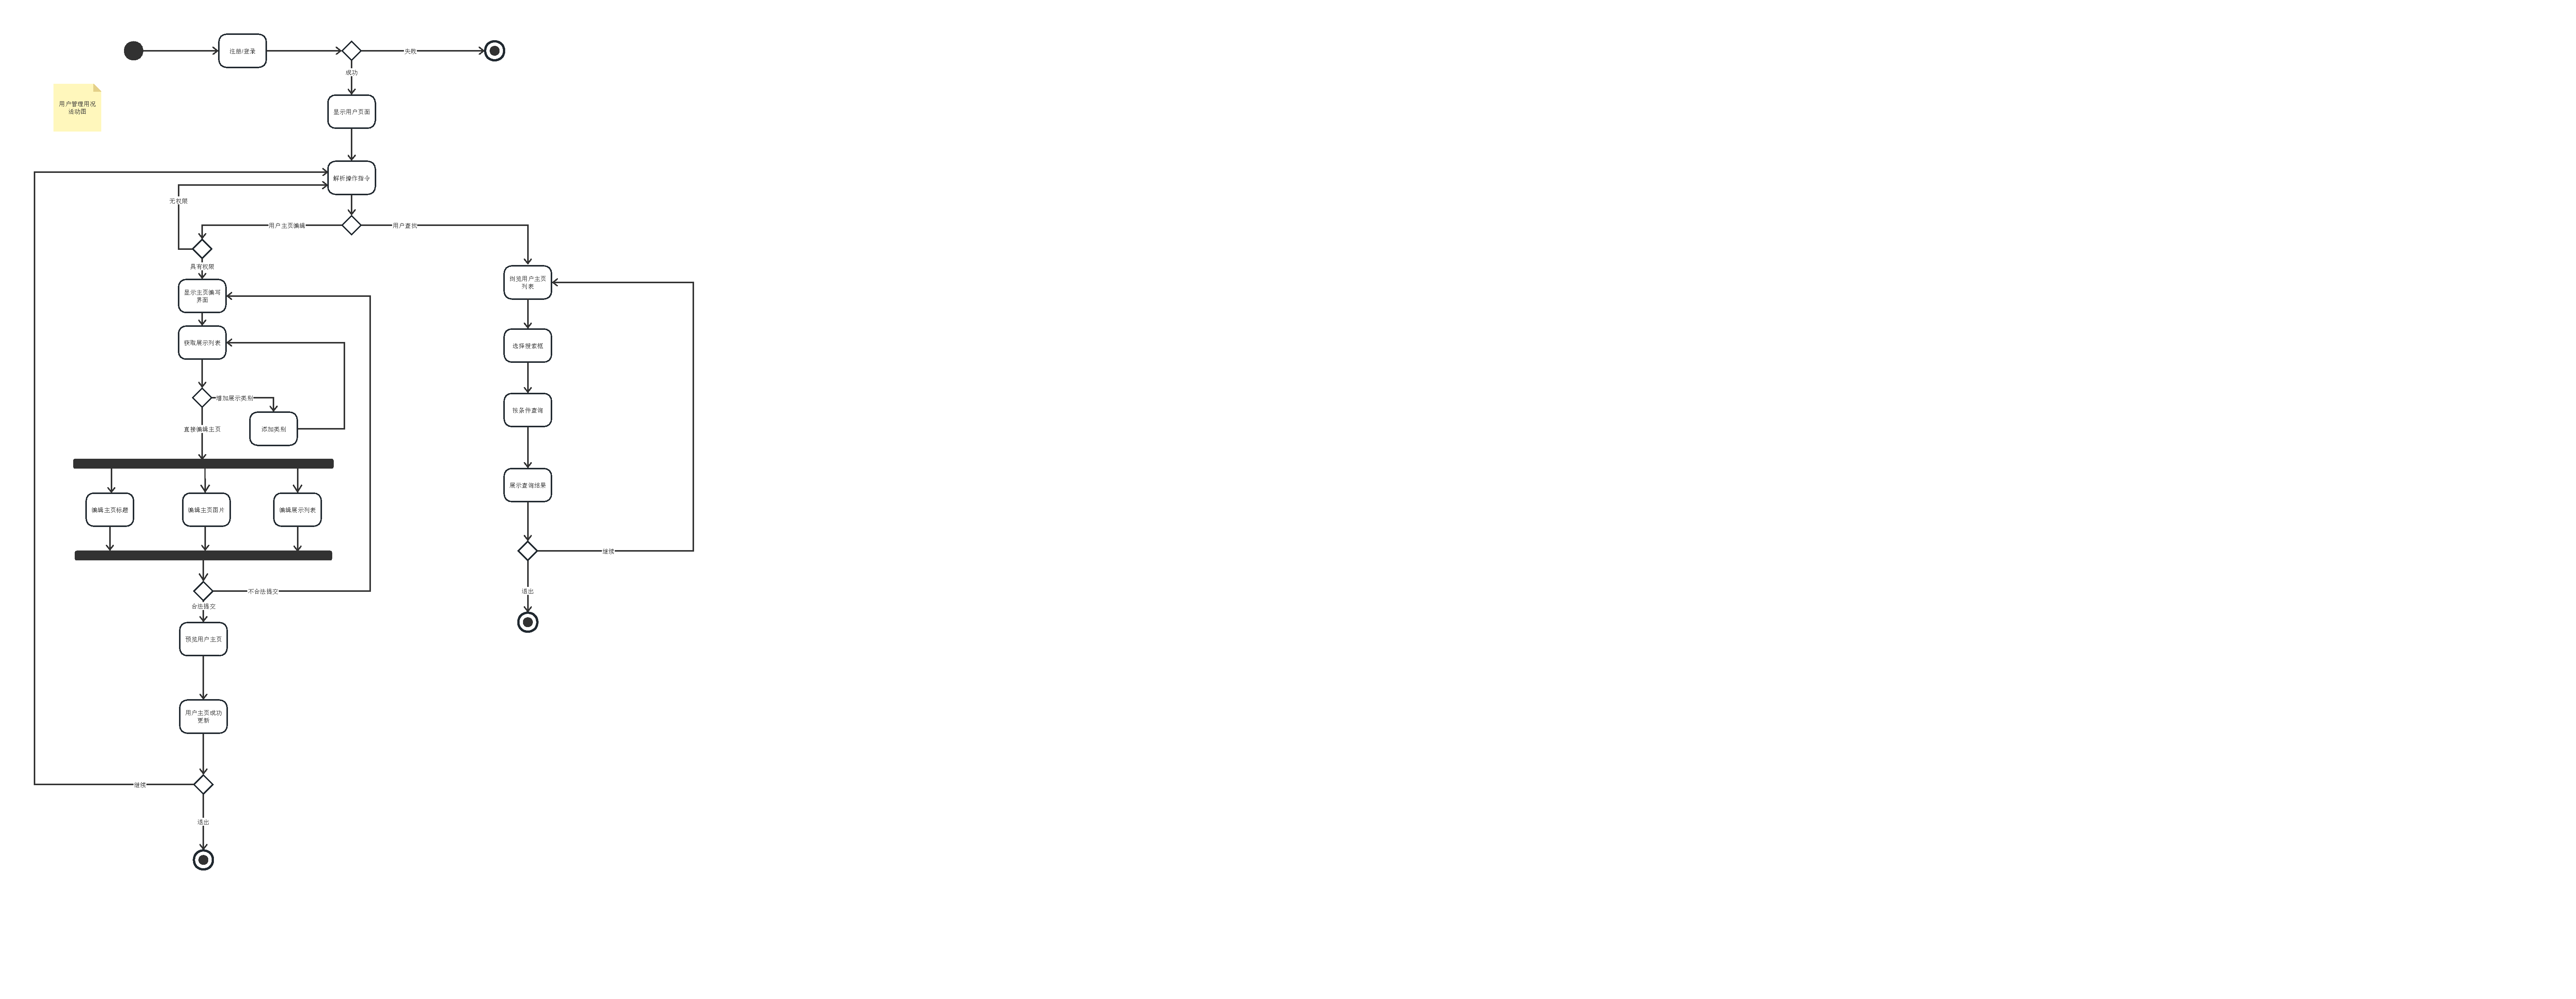
\includegraphics[scale=0.4]{OOA/fig/1-信息管理/信息管理用况活动图-1.pdf}} 
    \bicaption{Volunet信息管理系统用况活动1子图}{Activity 1 Subgraph for Information Management System Usage of Volunet} 
\end{figure}

\begin{figure}[H] 
    \center{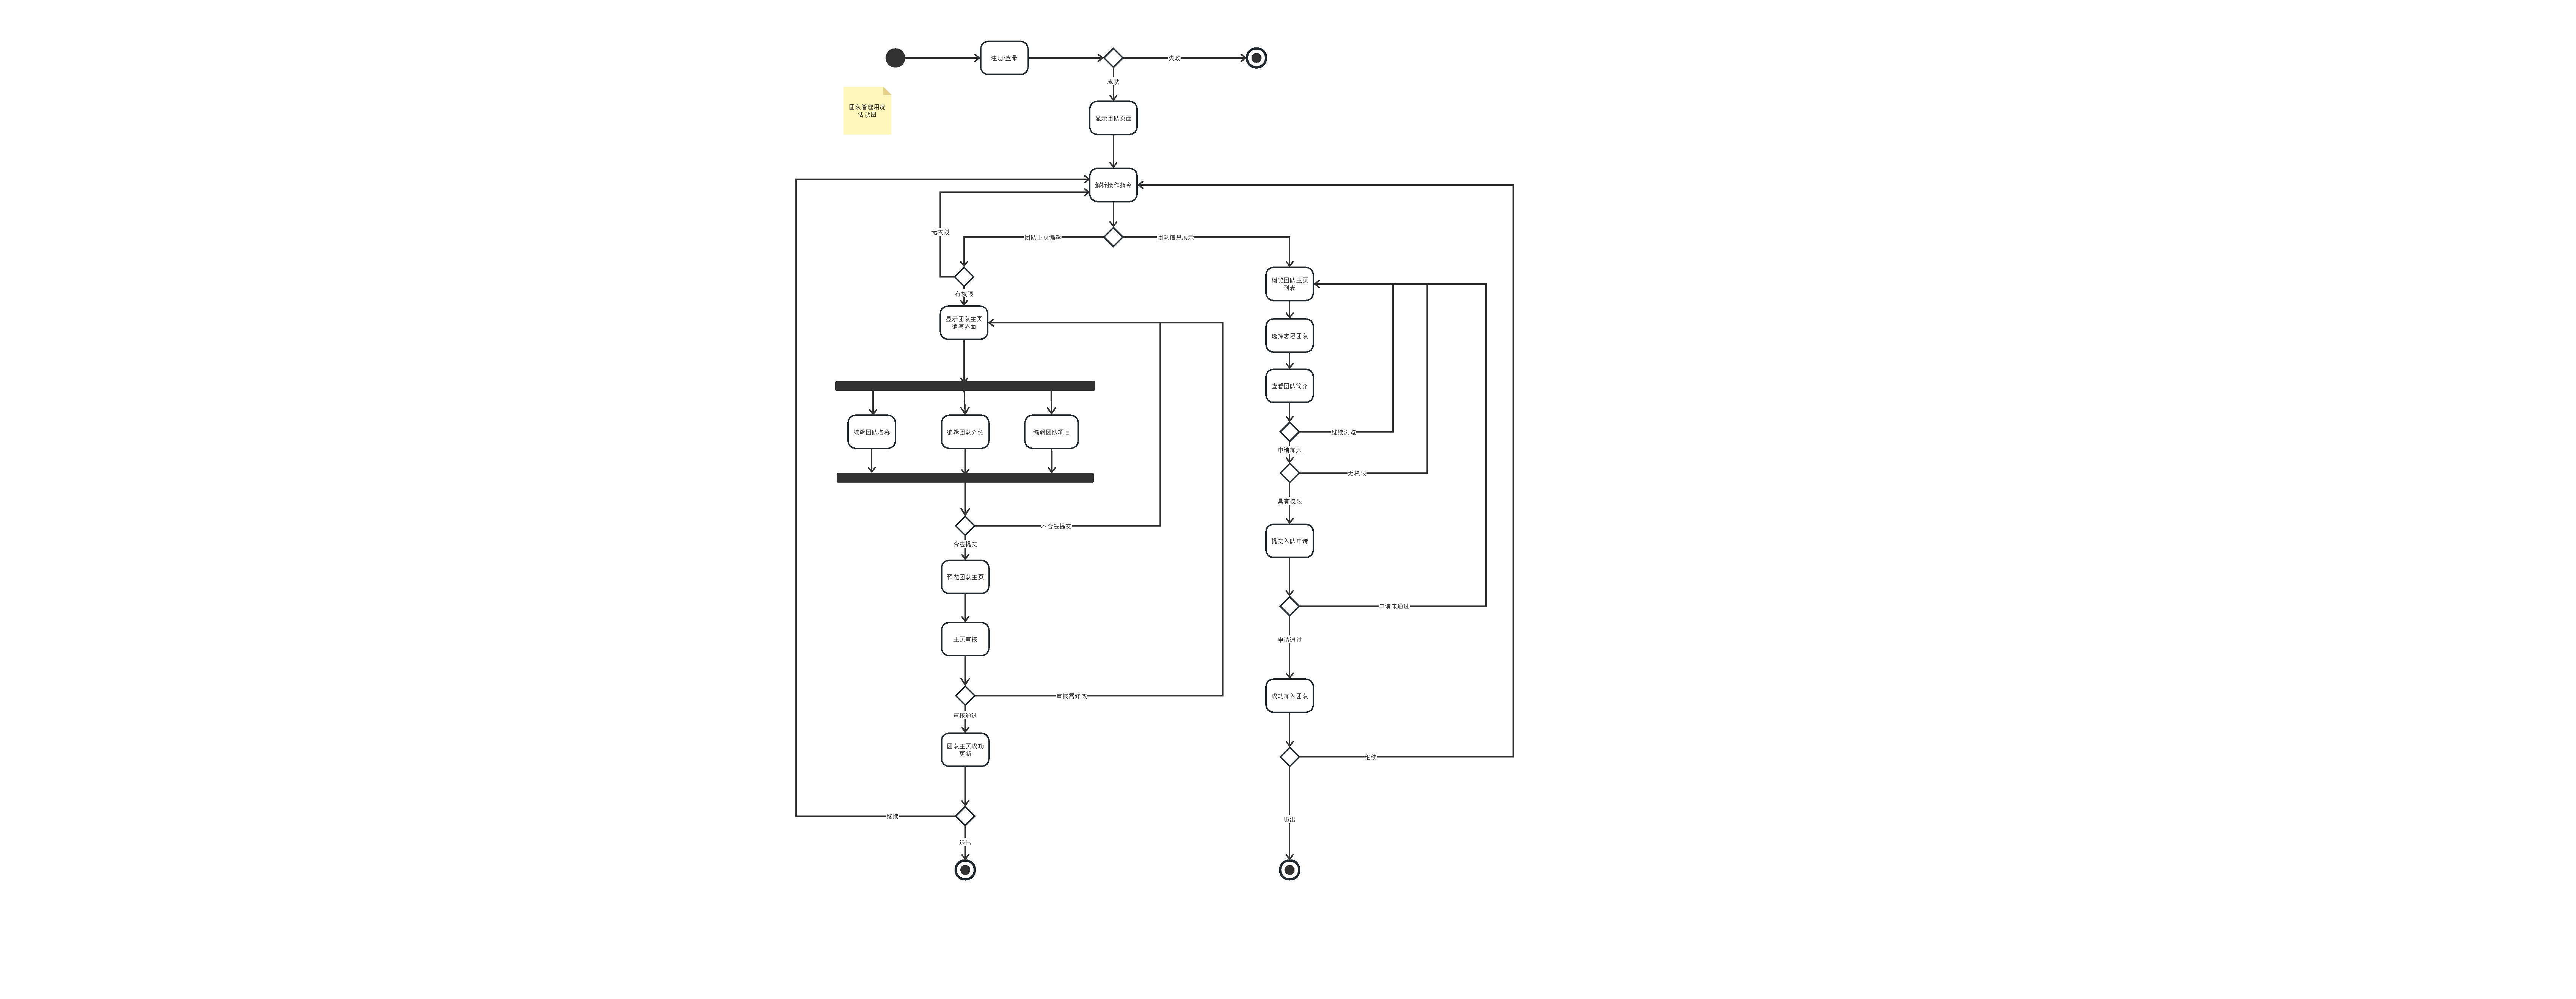
\includegraphics[scale=0.4]{OOA/fig/1-信息管理/信息管理用况活动图-2.pdf}} 
    \bicaption{Volunet信息管理系统用况活动2子图}{Activity 2 Subgraph for Information Management System Usage of Volunet} 
\end{figure}

\begin{figure}[H] 
    \center{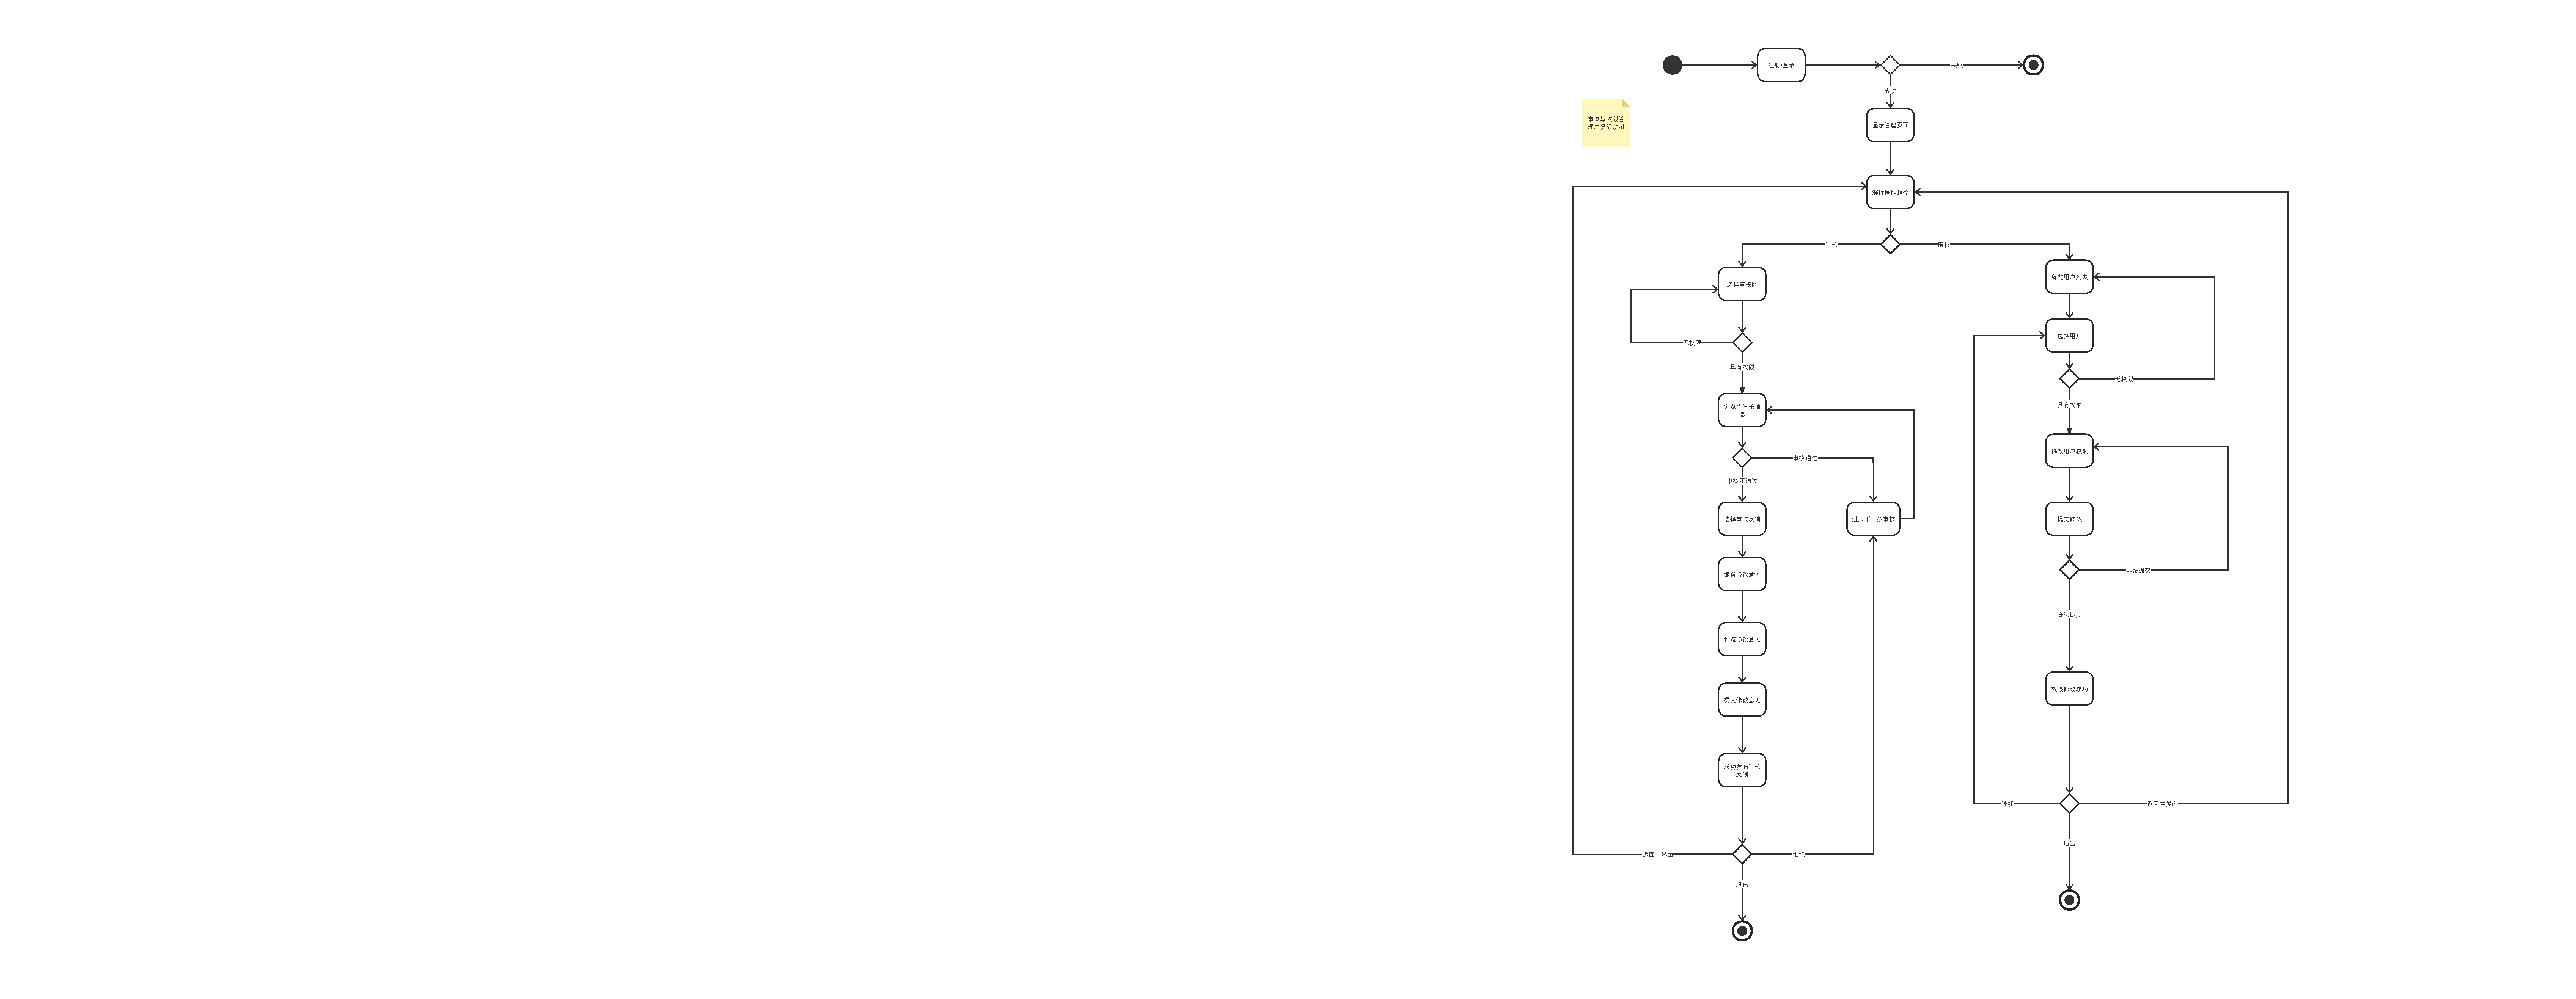
\includegraphics[scale=0.4]{OOA/fig/1-信息管理/信息管理用况活动图-3.pdf}} 
    \bicaption{Volunet信息管理系统用况活动3子图}{Activity 3 Subgraph for Information Management System Usage of Volunet} 
\end{figure}

\quad
\subsubsection{志愿服务系统}

\begin{figure}[H] 
    \center{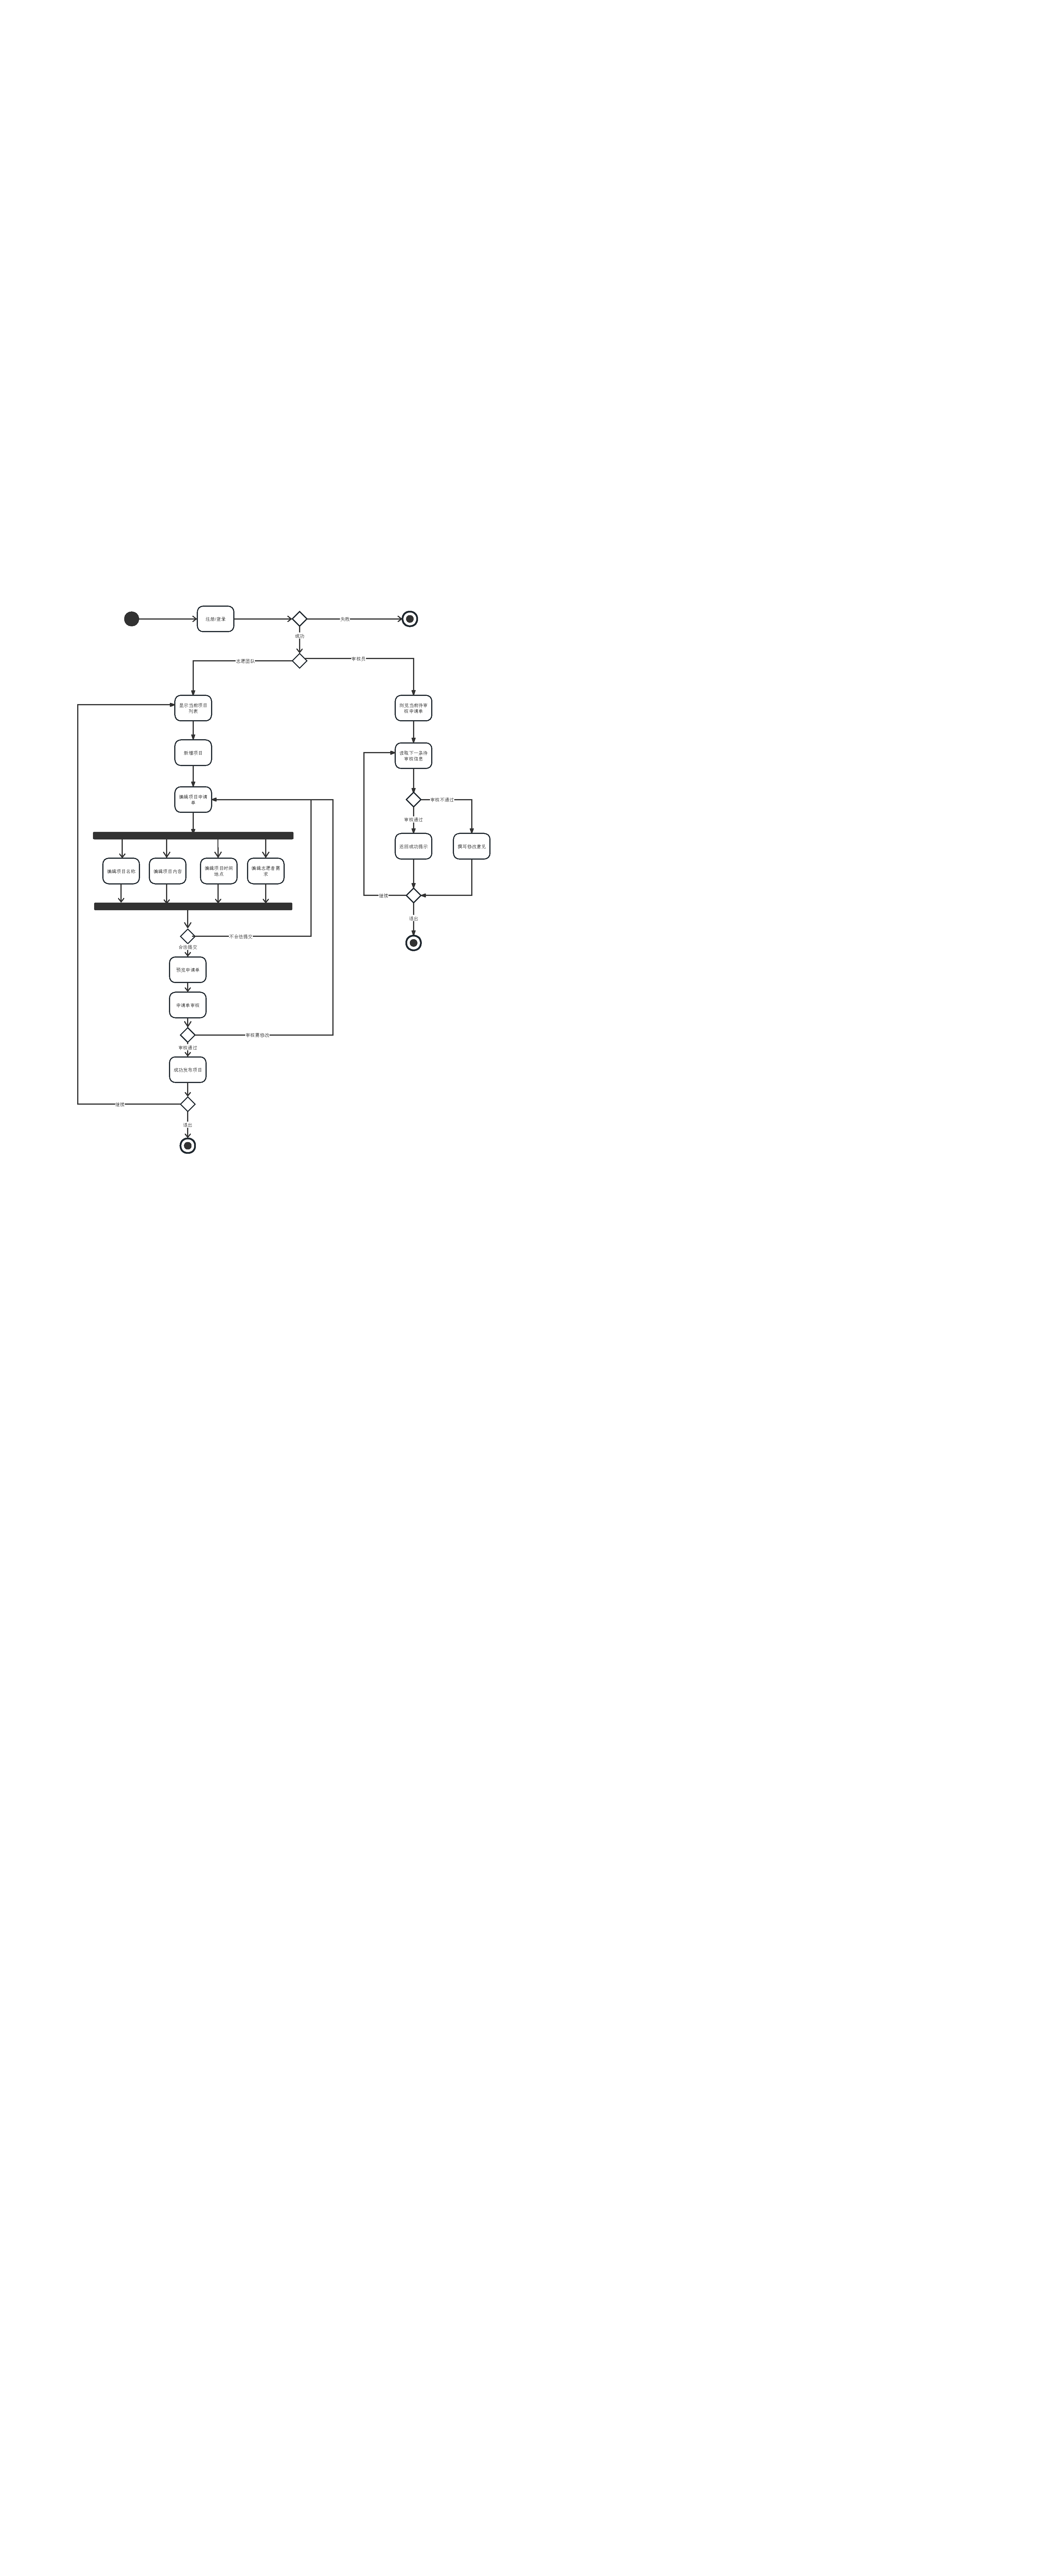
\includegraphics[scale=0.4]{OOA/fig/2-志愿服务/VS-用况活动图1.pdf}} 
    \bicaption{Volunet志愿服务系统用况活动1子图}{Activity 1 Subgraph for Voluntary Service System Usage of Volunet} 
\end{figure}

\begin{figure}[H] 
    \center{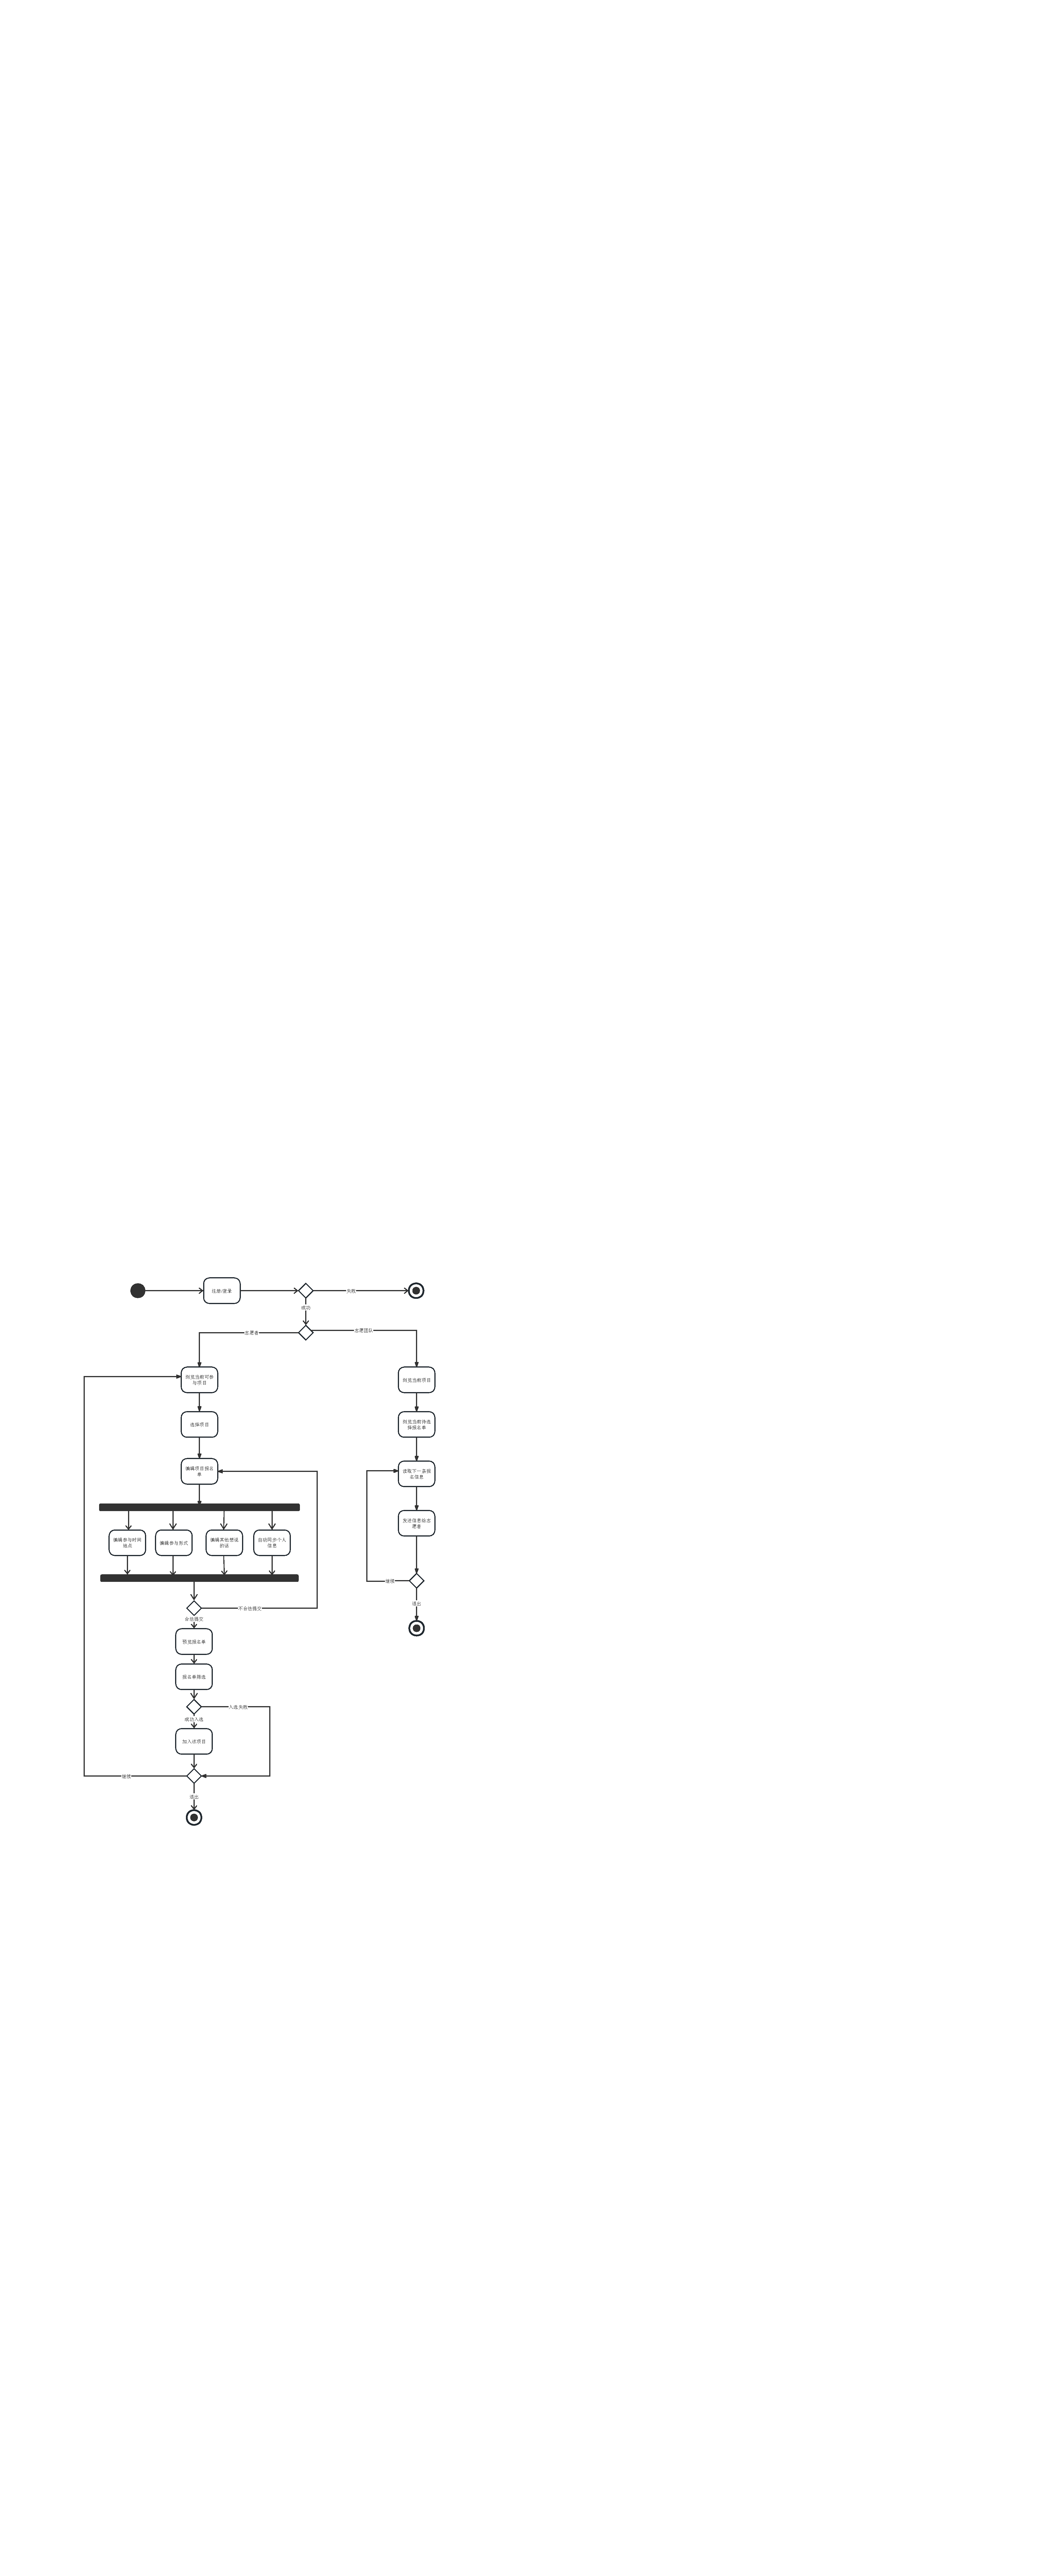
\includegraphics[scale=0.4]{OOA/fig/2-志愿服务/VS-用况活动图2.pdf}} 
    \bicaption{Volunet志愿服务系统用况活动2子图}{Activity 2 Subgraph for Voluntary Service System Usage of Volunet} 
\end{figure}

\begin{figure}[H] 
    \center{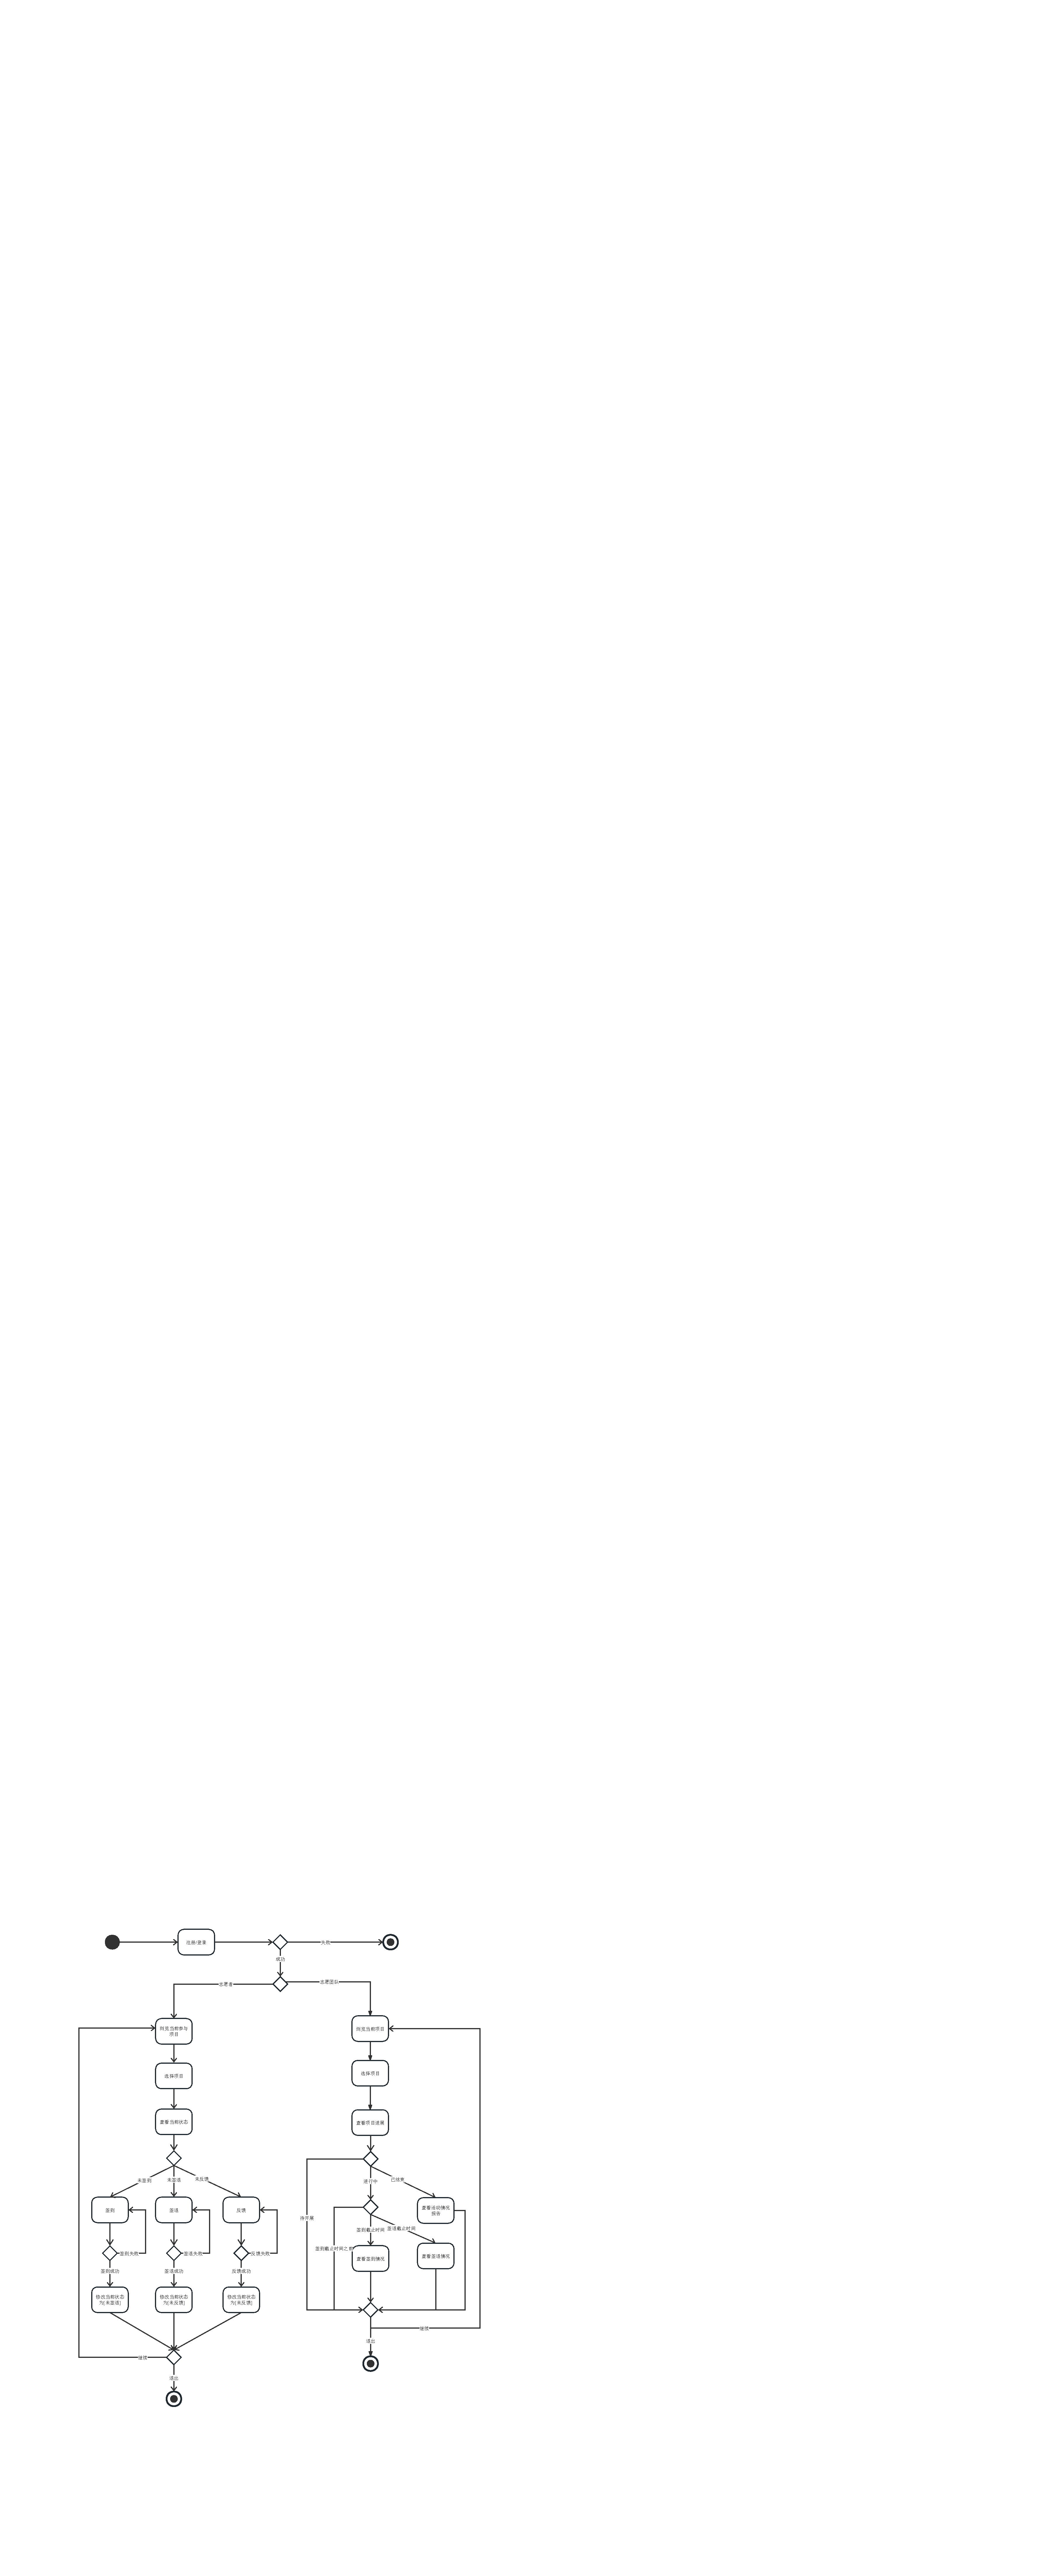
\includegraphics[scale=0.4]{OOA/fig/2-志愿服务/VS-用况活动图3.pdf}} 
    \bicaption{Volunet志愿服务系统用况活动3子图}{Activity 3 Subgraph for Voluntary Service System Usage of Volunet} 
\end{figure}


\subsubsection{爱心捐助系统}
\begin{figure}[H] 
    \center{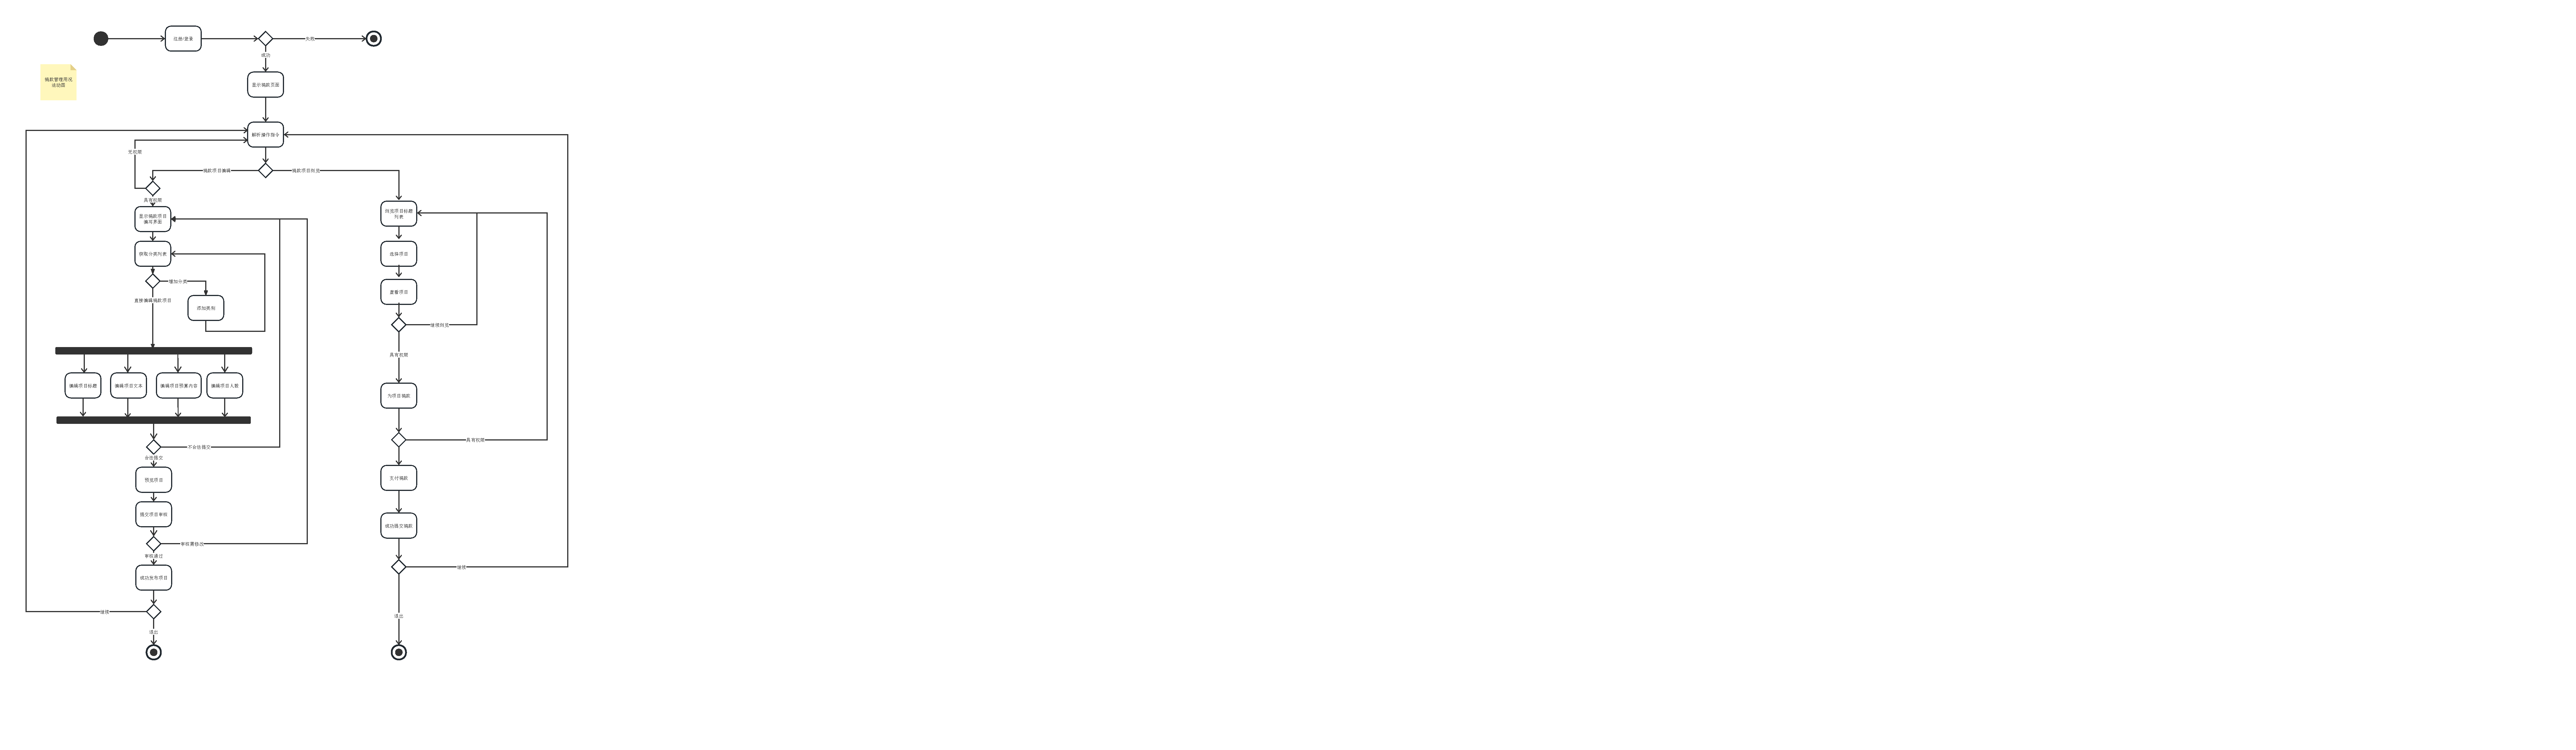
\includegraphics[scale=0.4]{OOA/fig/3-爱心管理/爱心管理用况活动图-1.pdf}} 
    \bicaption{Volunet爱心捐助系统用况活动1子图}{Activity 1 Subgraph for Love Donation System Usage of Volunet} 
\end{figure}
\quad
\begin{figure}[H] 
    \center{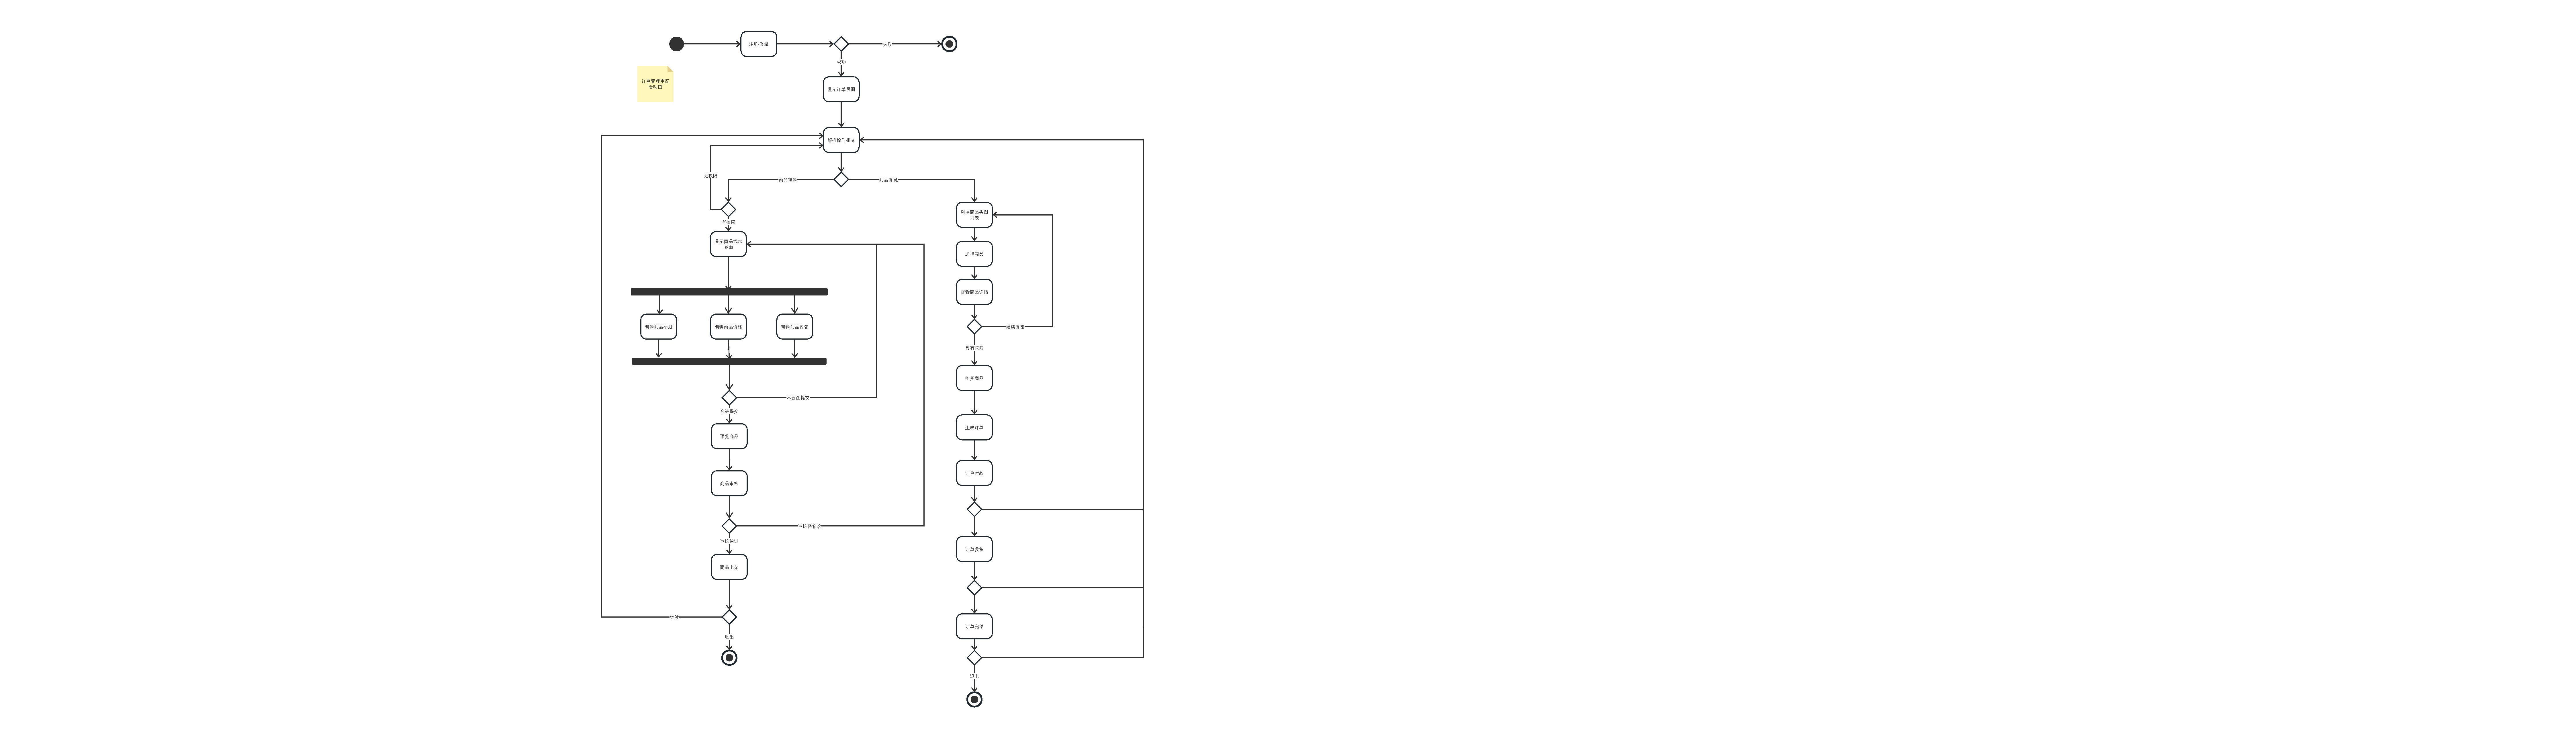
\includegraphics[scale=0.4]{OOA/fig/3-爱心管理/爱心管理用况活动图-2.pdf}} 
    \bicaption{Volunet爱心捐助系统用况活动2子图}{Activity 2 Subgraph for Love Donation System Usage of Volunet} 
\end{figure}

\begin{figure}[H] 
    \center{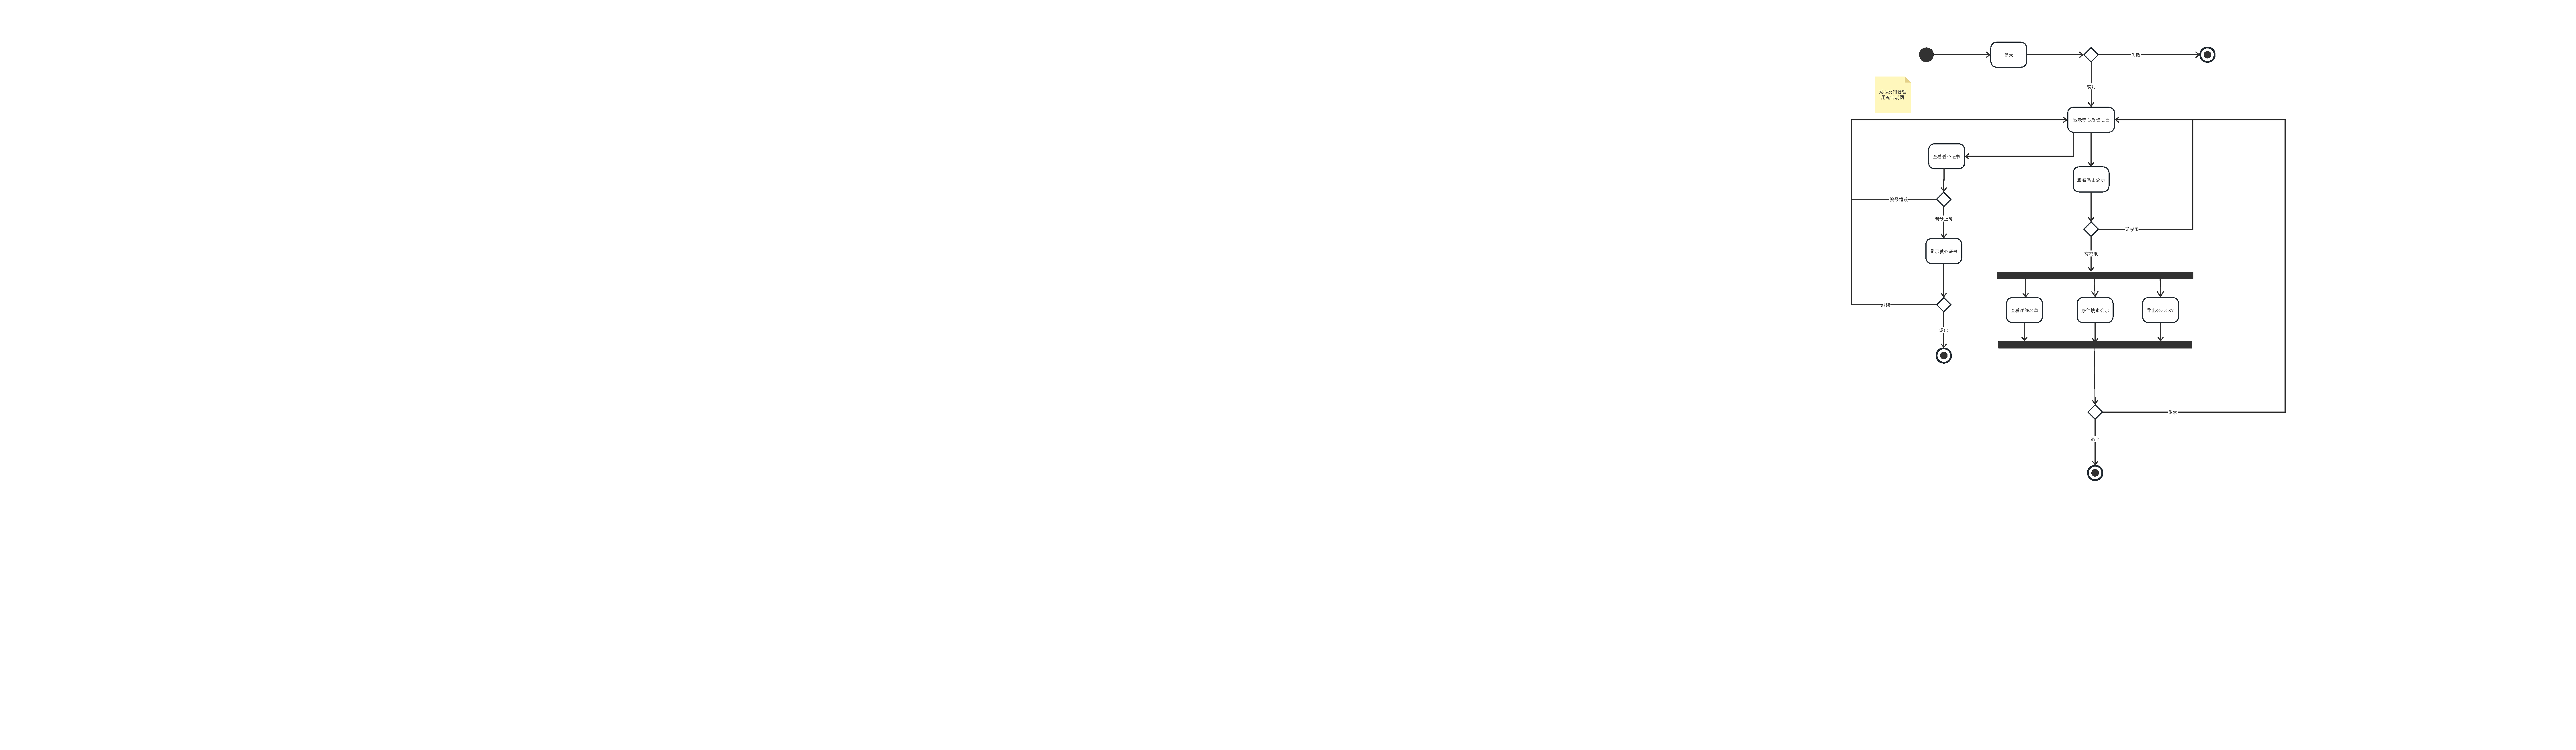
\includegraphics[scale=0.5]{OOA/fig/3-爱心管理/爱心管理用况活动图-3.pdf}} 
    \bicaption{Volunet爱心捐助系统用况活动3子图}{Activity 3 Subgraph for Love Donation System Usage of Volunet} 
\end{figure}

\subsubsection{公益课程系统}
\begin{figure}[H] 
    \center{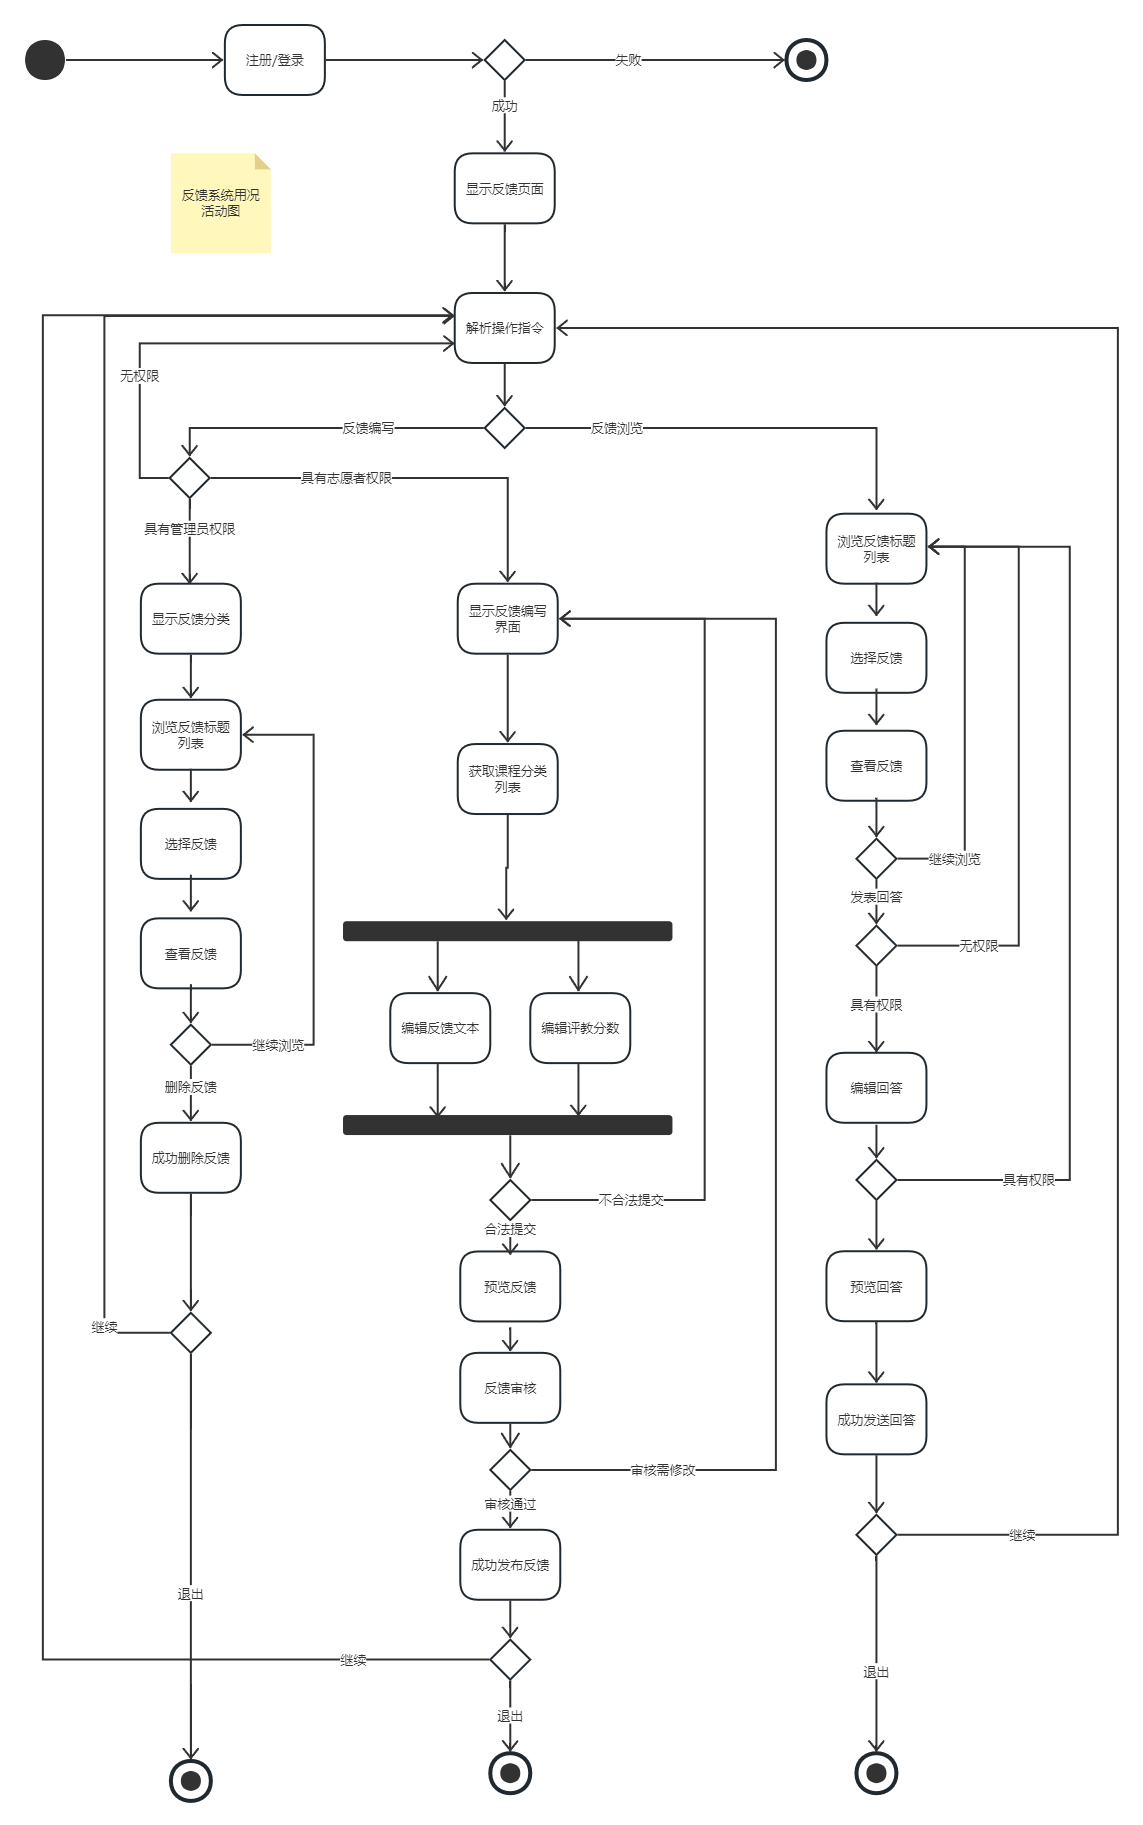
\includegraphics[scale=0.25]{OOA/fig/4-课程管理/课程管理用况活动图.png}} 
    \bicaption{Volunet公益课程系统用况活动1子图}{Activity 1 Subgraph for Course System Usage of Volunet} 
\end{figure}

\begin{figure}[H] 
    \center{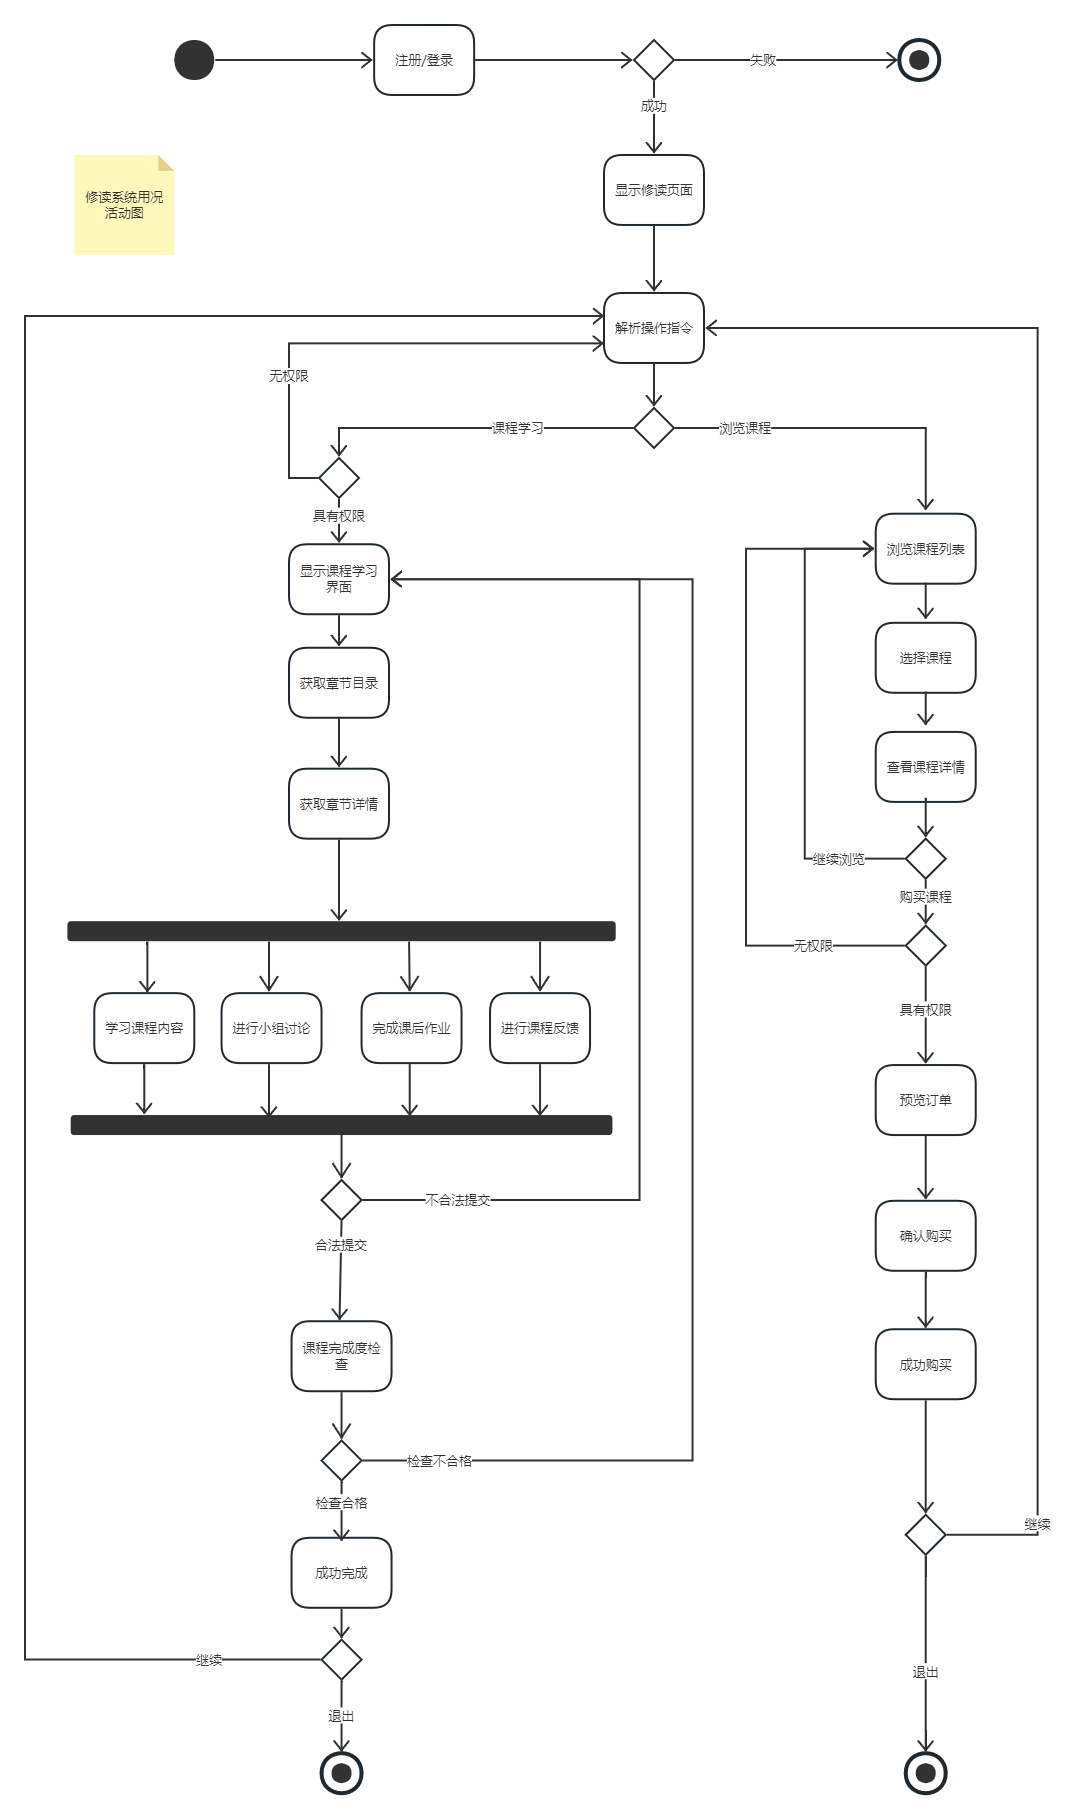
\includegraphics[scale=0.35]{OOA/fig/4-课程管理/课程管理用况活动图 (1).png}} 
    \bicaption{Volunet公益课程系统用况活动2子图}{Activity 2 Subgraph for Course System Usage of Volunet} 
\end{figure}

\begin{figure}[H] 
    \center{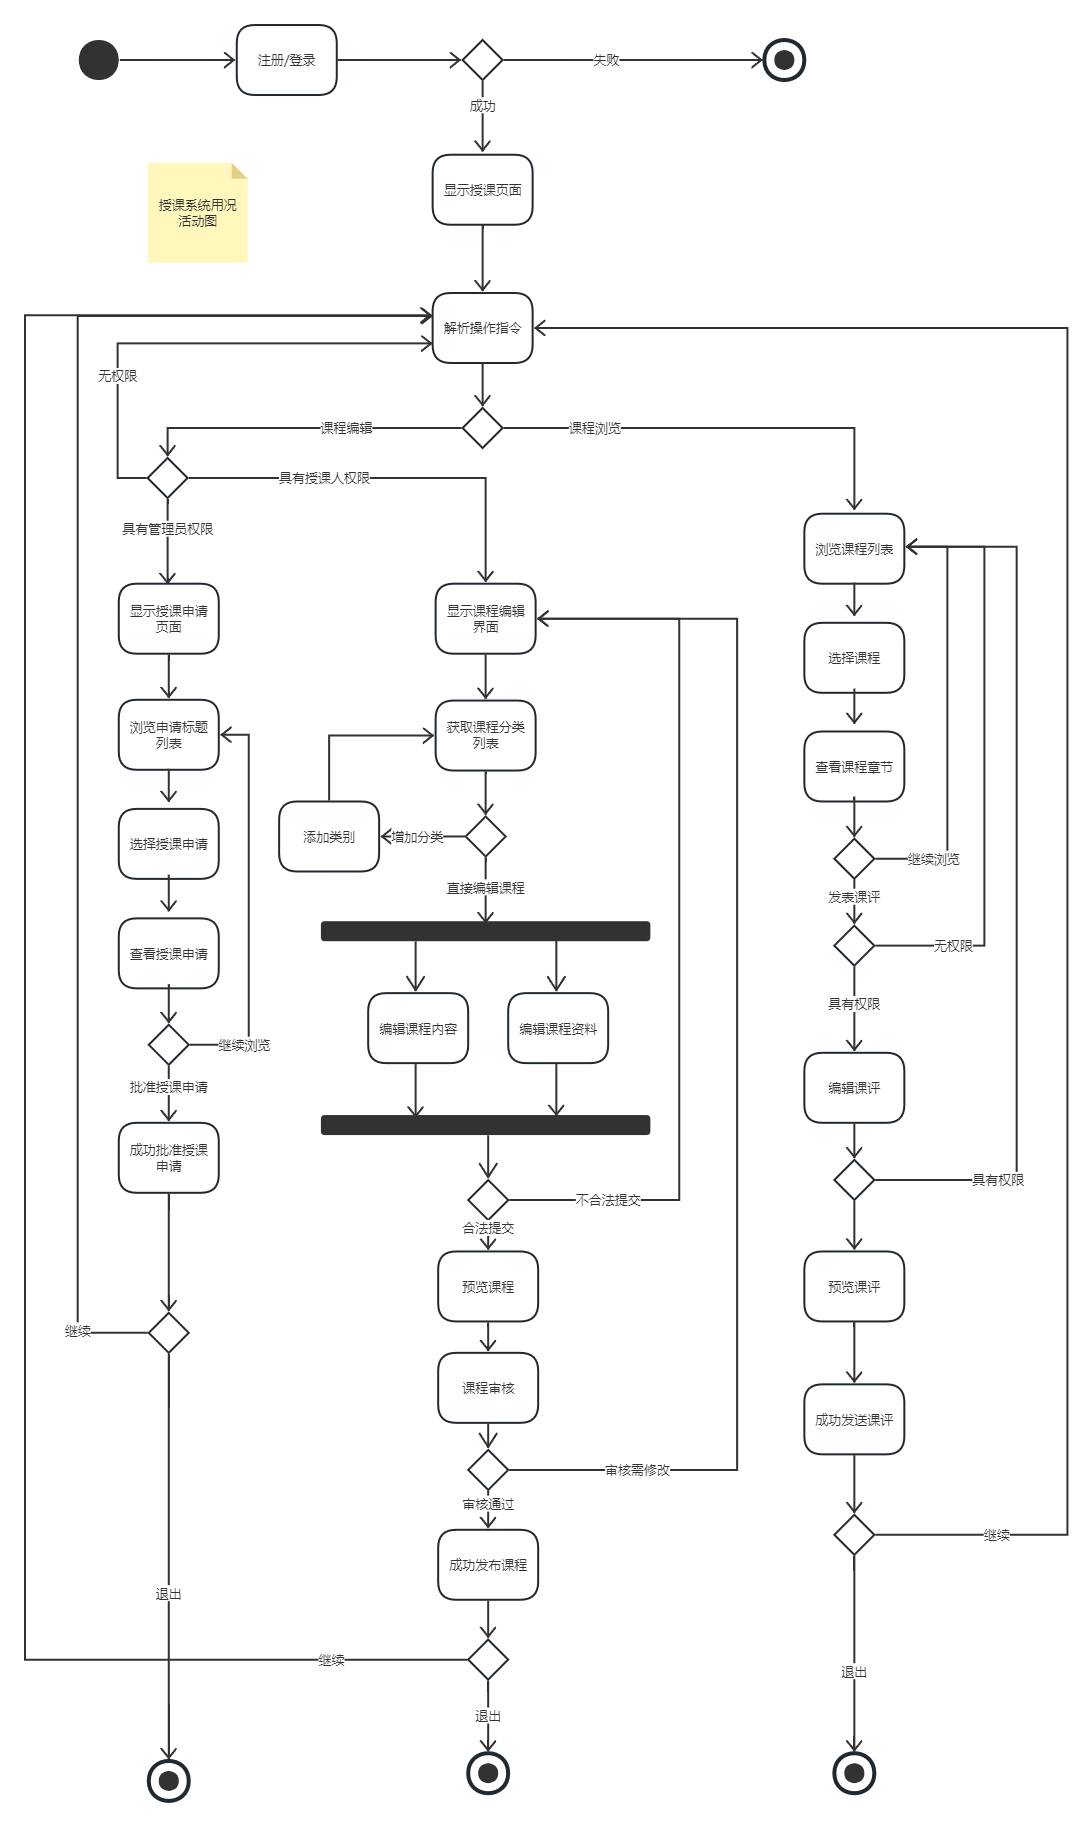
\includegraphics[scale=0.35]{OOA/fig/4-课程管理/课程管理用况活动图 (2).png}} 
    \bicaption{Volunet公益课程系统用况活动3子图}{Activity 3 Subgraph for Course System Usage of Volunet} 
\end{figure}

\subsubsection{交流论坛系统}
\begin{figure}[H] 
    \center{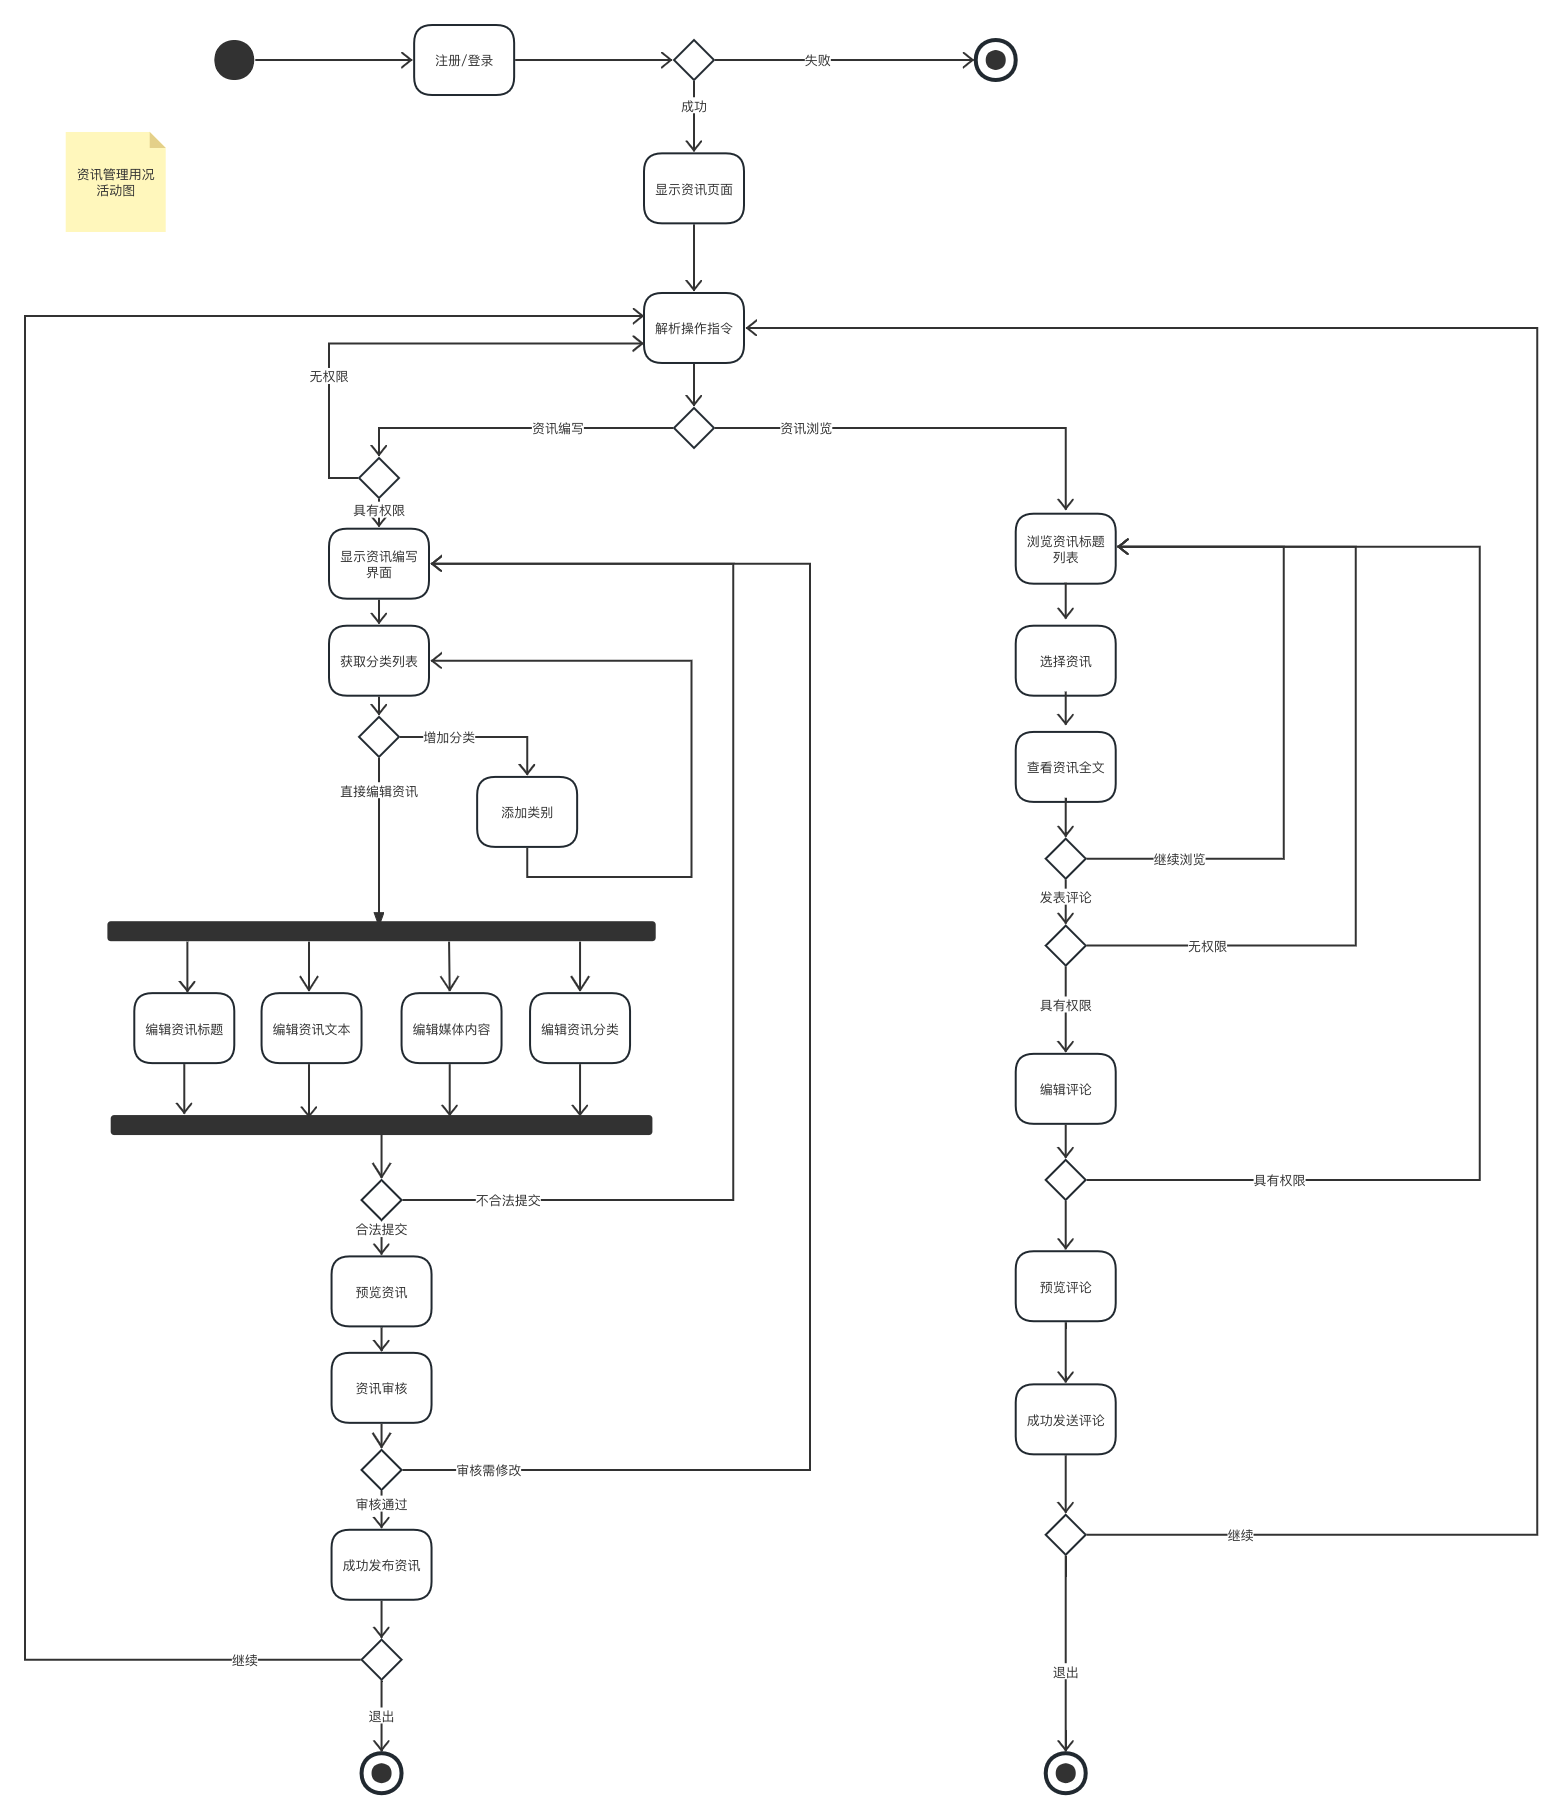
\includegraphics[scale=0.25]{OOA/fig/5-论坛管理/论坛管理用况活动图-1.png}} 
    \bicaption{Volunet交流论坛系统用况活动1子图}{Activity 1 Subgraph for Communication System Use Case of Volunet} 
\end{figure}

\begin{figure}[H] 
    \center{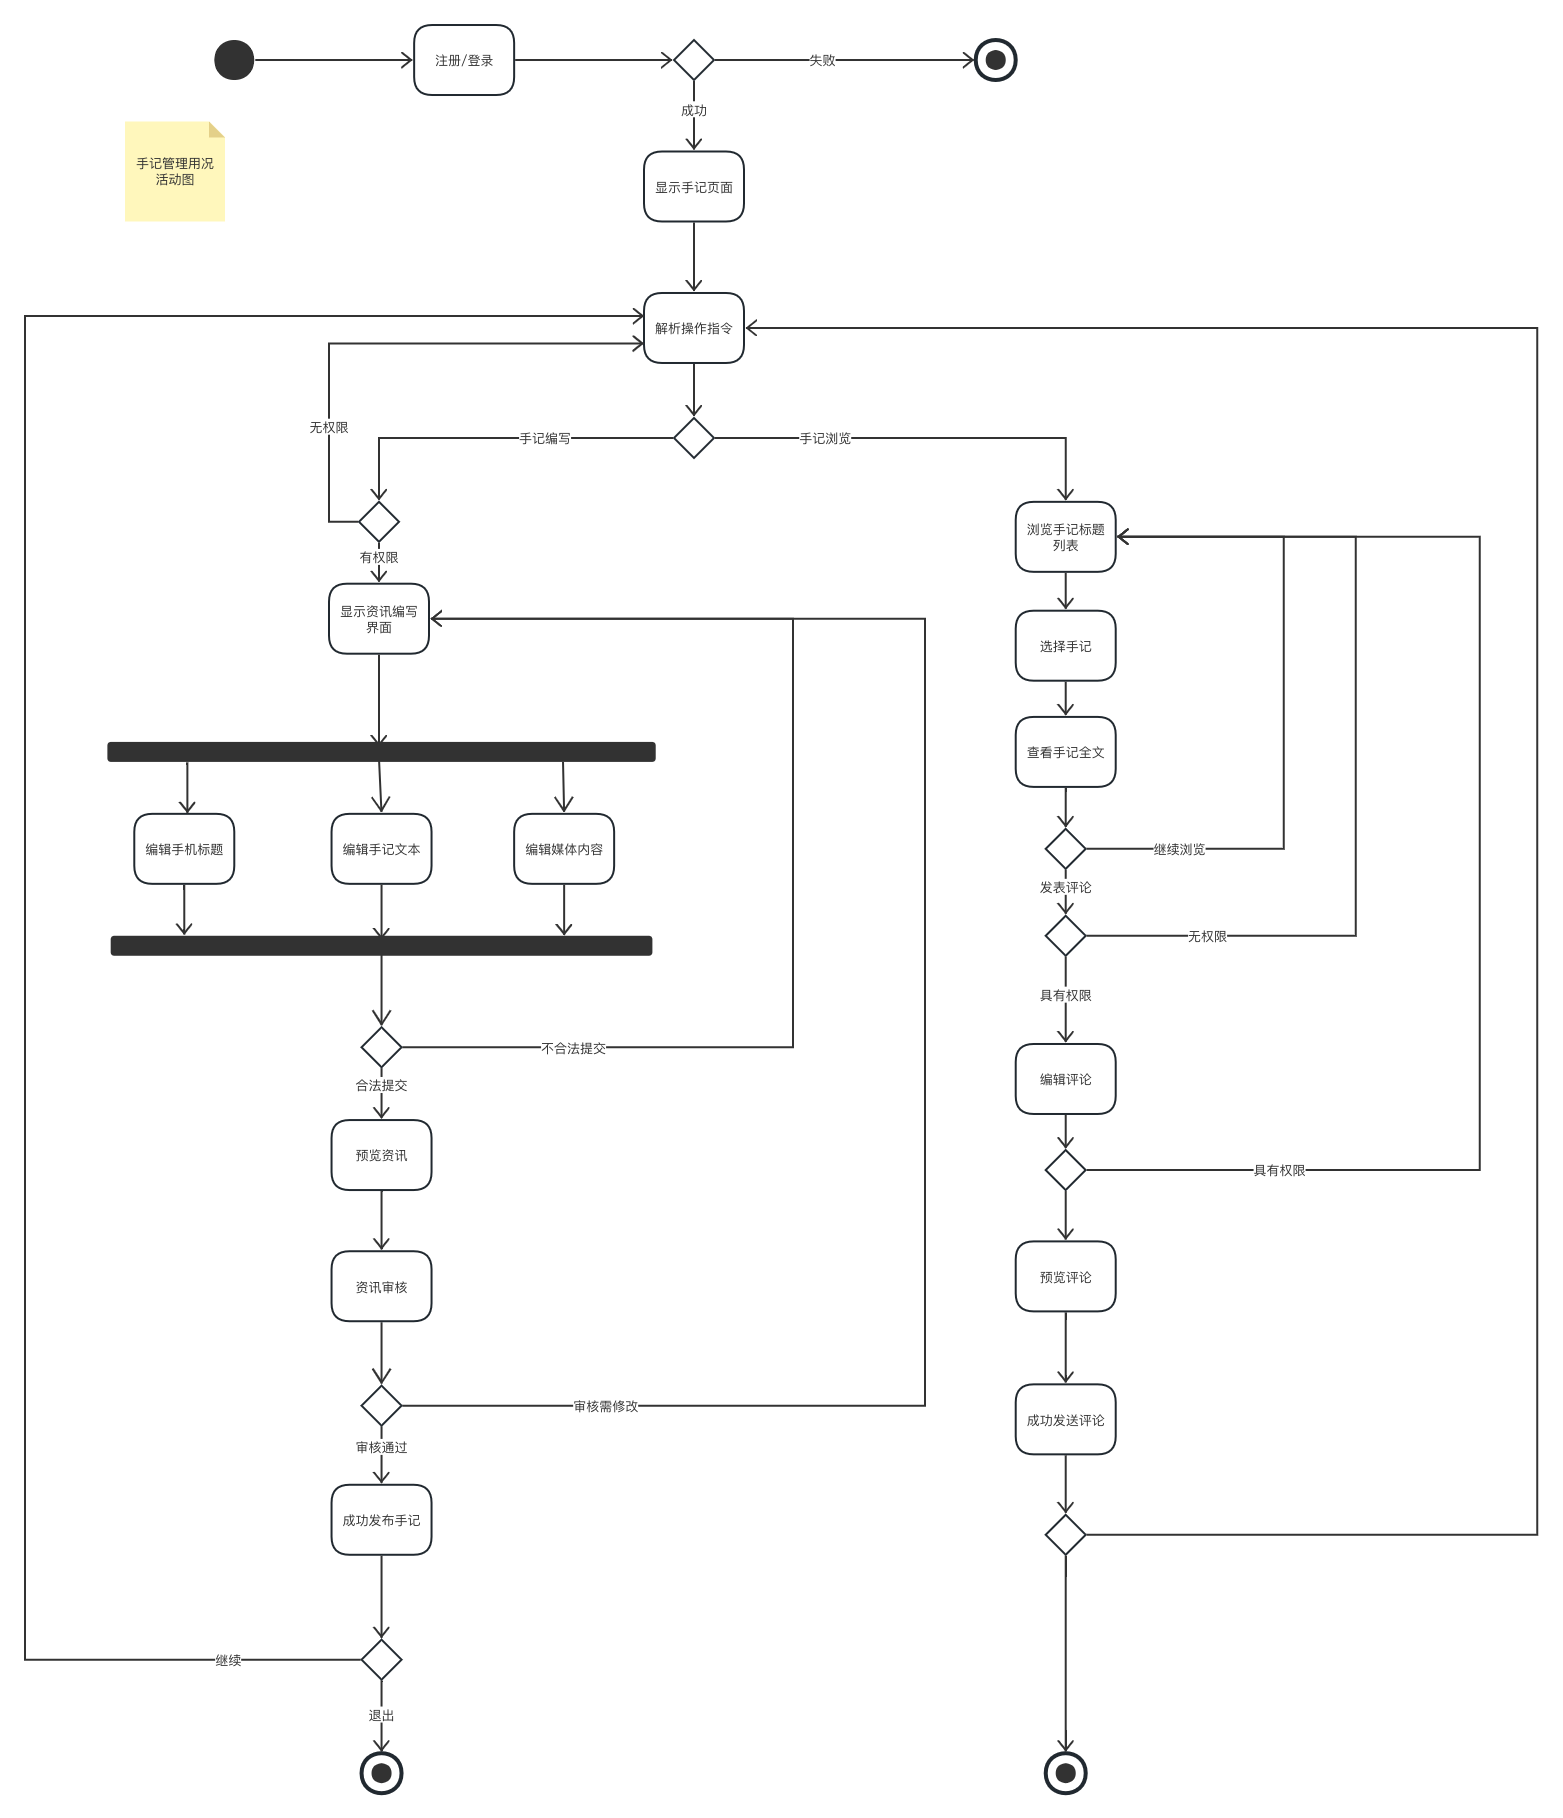
\includegraphics[scale=0.25]{OOA/fig/5-论坛管理/论坛管理用况活动图-2.png}} 
    \bicaption{Volunet交流论坛系统用况活动2子图}{Activity 2 Subgraph for Communication System Use Case of Volunet} 
\end{figure}

\begin{figure}[H] 
    \center{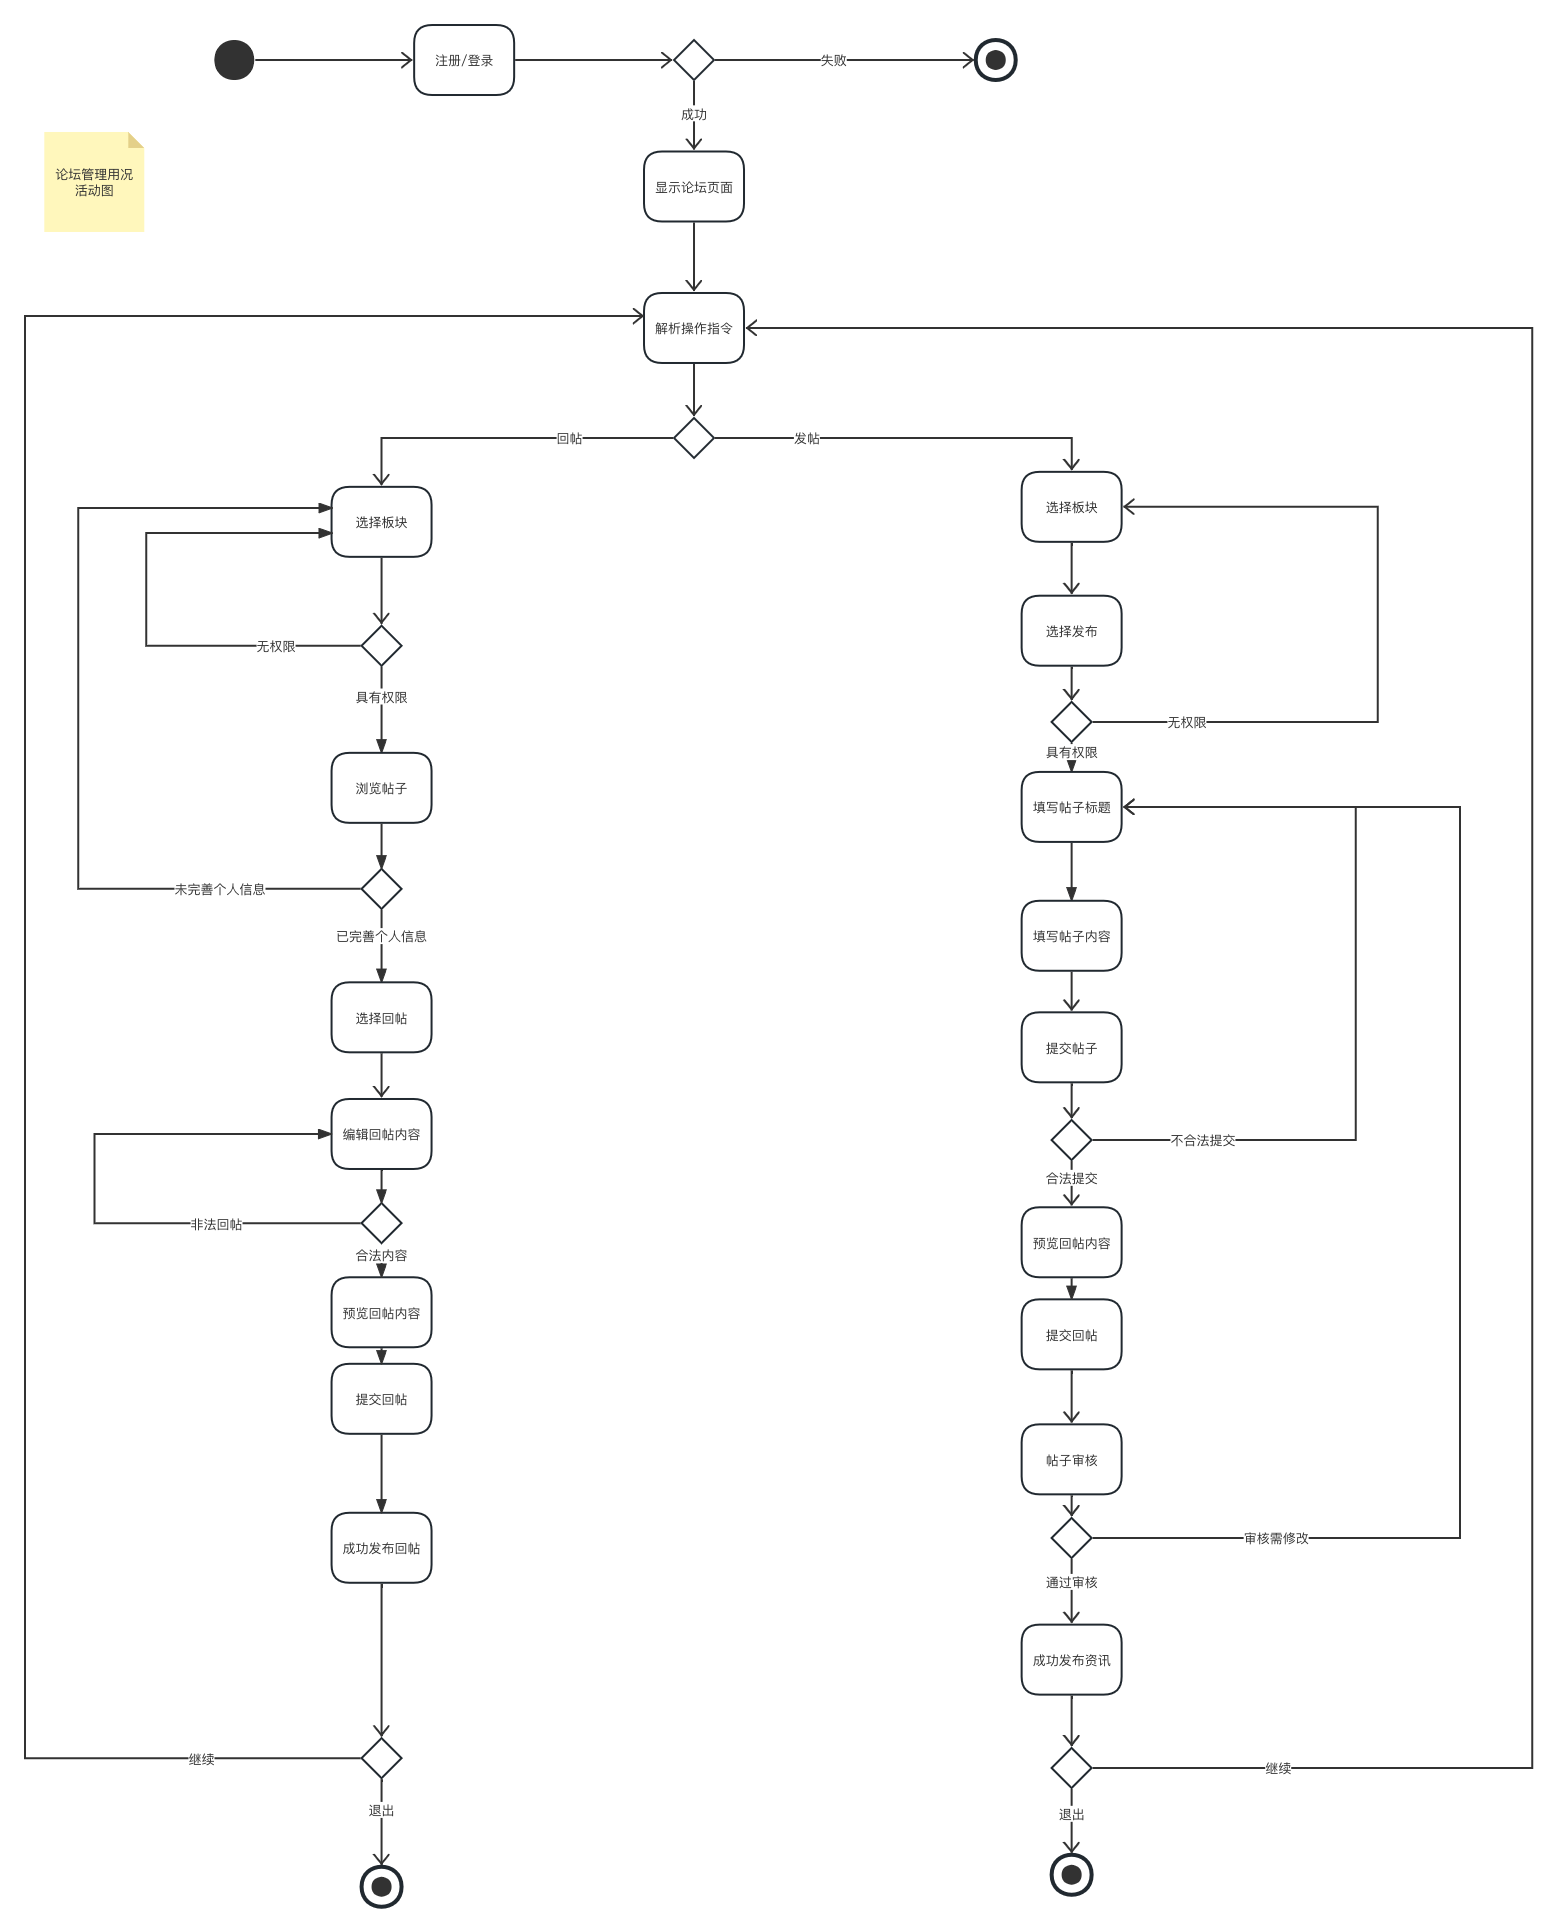
\includegraphics[scale=0.25]{OOA/fig/5-论坛管理/论坛管理用况活动图-3.png}} 
    \bicaption{Volunet交流论坛系统用况活动3子图}{Activity 3 Subgraph for Communication System Use Case of Volunet} 
\end{figure}

\begin{figure}[H] 
    \center{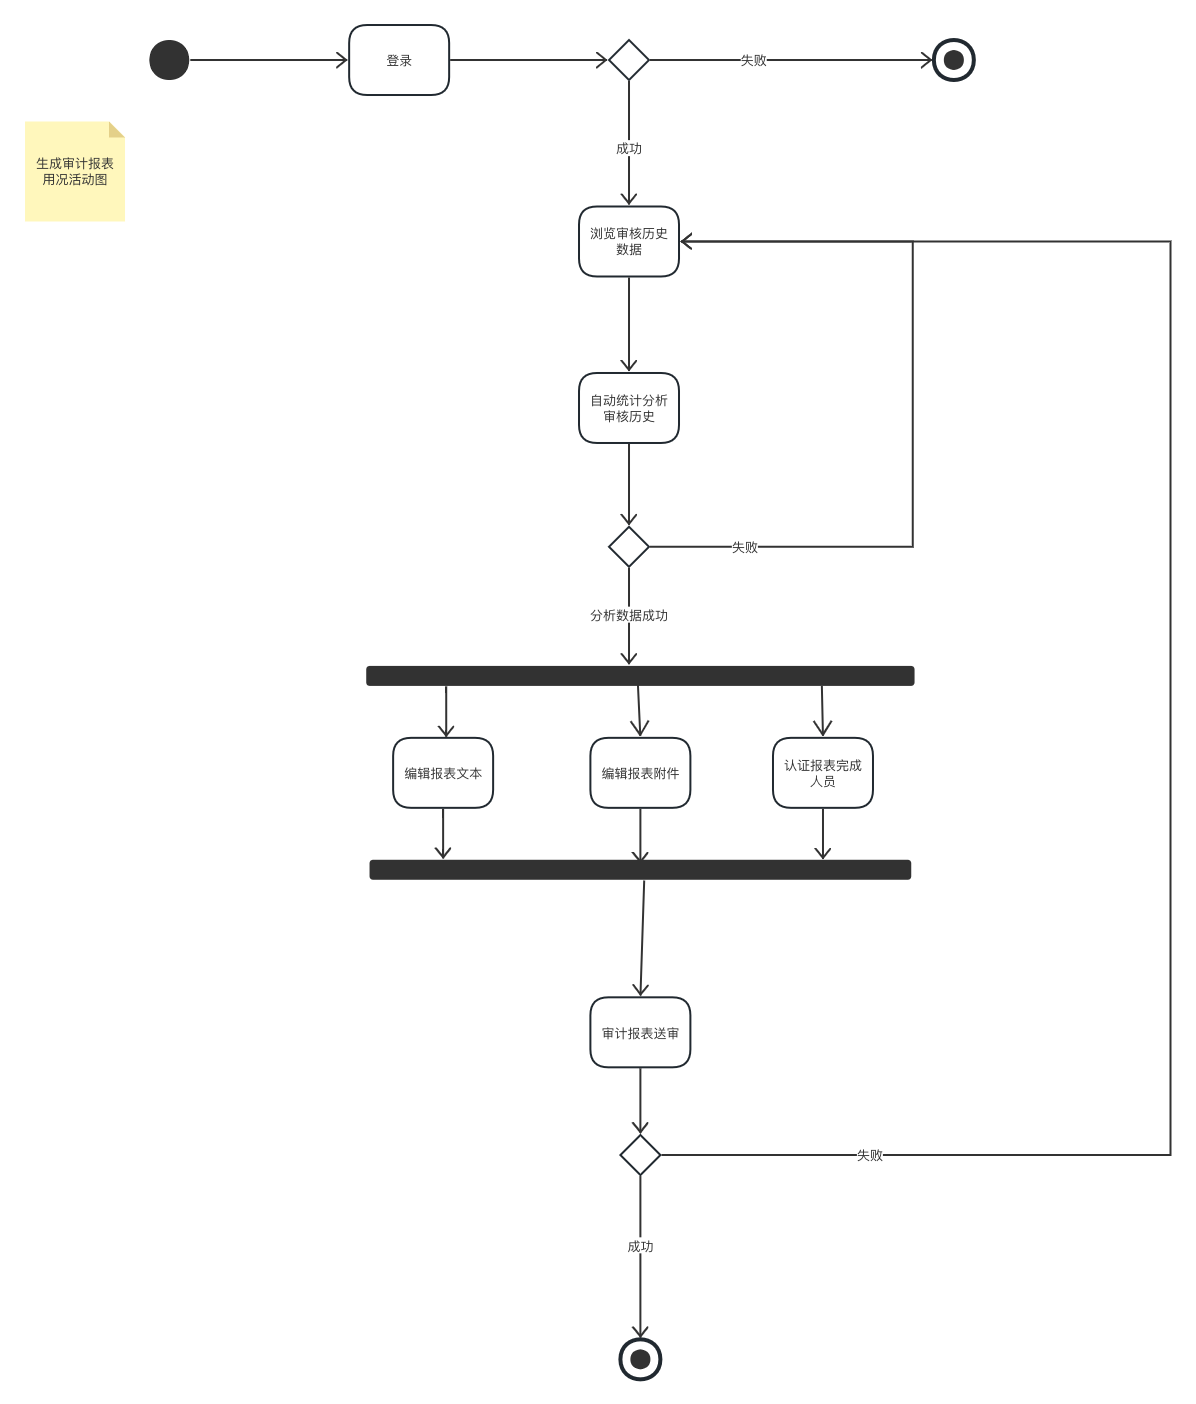
\includegraphics[scale=0.25]{OOA/fig/5-论坛管理/论坛管理用况活动图-4.png}} 
    \bicaption{Volunet交流论坛系统用况活动4子图}{Activity 4 Subgraph for Communication System Use Case of Volunet} 
\end{figure}

\subsubsection{志愿交友系统}
\begin{figure}[H] 
    \center{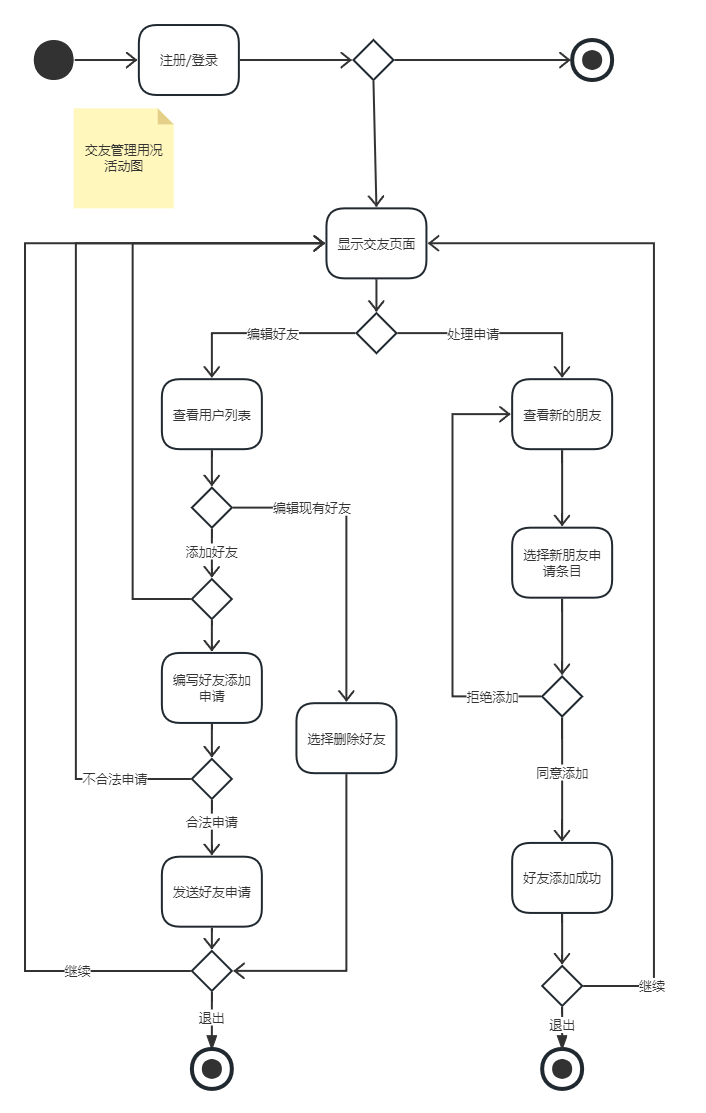
\includegraphics[scale=0.4]{OOA/fig/6-交友管理/志愿交友管理用况活动图.png}} 
    \bicaption{Volunet志愿交友系统用况活动1子图}{Activity 1 Subgraph for Volunteer Friends System Usage of Volunet} 
\end{figure}

\begin{figure}[H] 
    \center{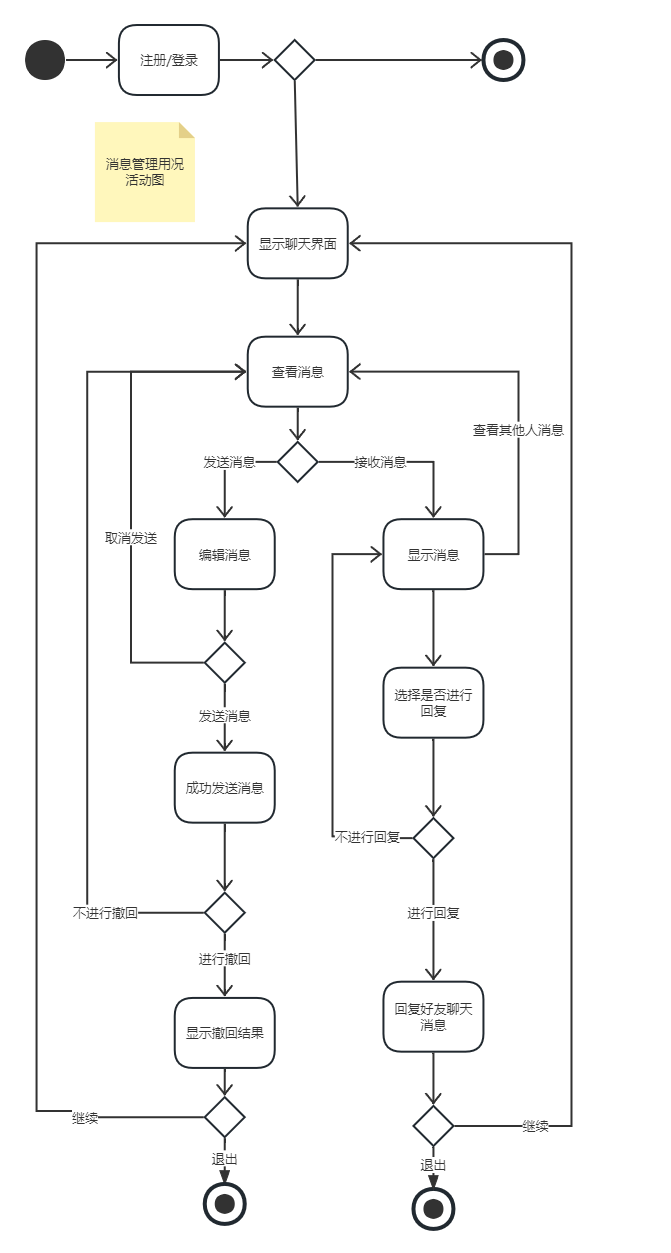
\includegraphics[scale=0.4]{OOA/fig/6-交友管理/志愿交友管理用况活动图 (1).png}} 
    \bicaption{Volunet志愿交友系统用况活动1子图}{Activity 1 Subgraph for Volunteer Friends System Usage of Volunet} 
\end{figure}














\newpage